% Options for packages loaded elsewhere
% Options for packages loaded elsewhere
\PassOptionsToPackage{unicode}{hyperref}
\PassOptionsToPackage{hyphens}{url}
\PassOptionsToPackage{dvipsnames,svgnames,x11names}{xcolor}
\PassOptionsToPackage{space}{xeCJK}
%
\documentclass[
  letterpaper,
  DIV=11,
  numbers=noendperiod]{scrartcl}
\usepackage{xcolor}
\usepackage{amsmath,amssymb}
\setcounter{secnumdepth}{-\maxdimen} % remove section numbering
\usepackage{iftex}
\ifPDFTeX
  \usepackage[T1]{fontenc}
  \usepackage[utf8]{inputenc}
  \usepackage{textcomp} % provide euro and other symbols
\else % if luatex or xetex
  \usepackage{unicode-math} % this also loads fontspec
  \defaultfontfeatures{Scale=MatchLowercase}
  \defaultfontfeatures[\rmfamily]{Ligatures=TeX,Scale=1}
\fi
\usepackage{lmodern}
\ifPDFTeX\else
  % xetex/luatex font selection
  \ifXeTeX
    \usepackage{xeCJK}
    \setCJKmainfont[BoldFont=STHeiti,ItalicFont=STKaiti]{STSong}
  \fi
  \ifLuaTeX
    \usepackage[]{luatexja-fontspec}
    \setmainjfont[BoldFont=STHeiti,ItalicFont=STKaiti]{STSong}
  \fi
\fi
% Use upquote if available, for straight quotes in verbatim environments
\IfFileExists{upquote.sty}{\usepackage{upquote}}{}
\IfFileExists{microtype.sty}{% use microtype if available
  \usepackage[]{microtype}
  \UseMicrotypeSet[protrusion]{basicmath} % disable protrusion for tt fonts
}{}
\makeatletter
\@ifundefined{KOMAClassName}{% if non-KOMA class
  \IfFileExists{parskip.sty}{%
    \usepackage{parskip}
  }{% else
    \setlength{\parindent}{0pt}
    \setlength{\parskip}{6pt plus 2pt minus 1pt}}
}{% if KOMA class
  \KOMAoptions{parskip=half}}
\makeatother
% Make \paragraph and \subparagraph free-standing
\makeatletter
\ifx\paragraph\undefined\else
  \let\oldparagraph\paragraph
  \renewcommand{\paragraph}{
    \@ifstar
      \xxxParagraphStar
      \xxxParagraphNoStar
  }
  \newcommand{\xxxParagraphStar}[1]{\oldparagraph*{#1}\mbox{}}
  \newcommand{\xxxParagraphNoStar}[1]{\oldparagraph{#1}\mbox{}}
\fi
\ifx\subparagraph\undefined\else
  \let\oldsubparagraph\subparagraph
  \renewcommand{\subparagraph}{
    \@ifstar
      \xxxSubParagraphStar
      \xxxSubParagraphNoStar
  }
  \newcommand{\xxxSubParagraphStar}[1]{\oldsubparagraph*{#1}\mbox{}}
  \newcommand{\xxxSubParagraphNoStar}[1]{\oldsubparagraph{#1}\mbox{}}
\fi
\makeatother


\usepackage{longtable,booktabs,array}
\usepackage{calc} % for calculating minipage widths
% Correct order of tables after \paragraph or \subparagraph
\usepackage{etoolbox}
\makeatletter
\patchcmd\longtable{\par}{\if@noskipsec\mbox{}\fi\par}{}{}
\makeatother
% Allow footnotes in longtable head/foot
\IfFileExists{footnotehyper.sty}{\usepackage{footnotehyper}}{\usepackage{footnote}}
\makesavenoteenv{longtable}
\usepackage{graphicx}
\makeatletter
\newsavebox\pandoc@box
\newcommand*\pandocbounded[1]{% scales image to fit in text height/width
  \sbox\pandoc@box{#1}%
  \Gscale@div\@tempa{\textheight}{\dimexpr\ht\pandoc@box+\dp\pandoc@box\relax}%
  \Gscale@div\@tempb{\linewidth}{\wd\pandoc@box}%
  \ifdim\@tempb\p@<\@tempa\p@\let\@tempa\@tempb\fi% select the smaller of both
  \ifdim\@tempa\p@<\p@\scalebox{\@tempa}{\usebox\pandoc@box}%
  \else\usebox{\pandoc@box}%
  \fi%
}
% Set default figure placement to htbp
\def\fps@figure{htbp}
\makeatother


% definitions for citeproc citations
\NewDocumentCommand\citeproctext{}{}
\NewDocumentCommand\citeproc{mm}{%
  \begingroup\def\citeproctext{#2}\cite{#1}\endgroup}
\makeatletter
 % allow citations to break across lines
 \let\@cite@ofmt\@firstofone
 % avoid brackets around text for \cite:
 \def\@biblabel#1{}
 \def\@cite#1#2{{#1\if@tempswa , #2\fi}}
\makeatother
\newlength{\cslhangindent}
\setlength{\cslhangindent}{1.5em}
\newlength{\csllabelwidth}
\setlength{\csllabelwidth}{3em}
\newenvironment{CSLReferences}[2] % #1 hanging-indent, #2 entry-spacing
 {\begin{list}{}{%
  \setlength{\itemindent}{0pt}
  \setlength{\leftmargin}{0pt}
  \setlength{\parsep}{0pt}
  % turn on hanging indent if param 1 is 1
  \ifodd #1
   \setlength{\leftmargin}{\cslhangindent}
   \setlength{\itemindent}{-1\cslhangindent}
  \fi
  % set entry spacing
  \setlength{\itemsep}{#2\baselineskip}}}
 {\end{list}}
\usepackage{calc}
\newcommand{\CSLBlock}[1]{\hfill\break\parbox[t]{\linewidth}{\strut\ignorespaces#1\strut}}
\newcommand{\CSLLeftMargin}[1]{\parbox[t]{\csllabelwidth}{\strut#1\strut}}
\newcommand{\CSLRightInline}[1]{\parbox[t]{\linewidth - \csllabelwidth}{\strut#1\strut}}
\newcommand{\CSLIndent}[1]{\hspace{\cslhangindent}#1}



\setlength{\emergencystretch}{3em} % prevent overfull lines

\providecommand{\tightlist}{%
  \setlength{\itemsep}{0pt}\setlength{\parskip}{0pt}}



 


\KOMAoption{captions}{tableheading}
% -- begin:latex-table-short-captions --
\makeatletter\AtBeginDocument{%
\def\LT@c@ption#1[#2]#3{%                 % Overwrite the workhorse macro used in formatting a longtable caption.
  \LT@makecaption#1\fnum@table{#3}%
  \@ifundefined{pandoctableshortcapt}
     {\def\@tempa{#2}}                    % Use default behaviour: argument in square brackets
     {\let\@tempa\pandoctableshortcapt}   % If defined (even if blank), use to override
  \ifx\@tempa\@empty\else                 % If @tempa is blank, no lot entry! Otherwise, @tempa becomes the lot title.
     {\let\\\space
     \addcontentsline{lot}{table}{\protect\numberline{\thetable}{\@tempa}}}%
  \fi}
}\makeatother
% -- end:latex-table-short-captions --
\makeatletter
\@ifpackageloaded{caption}{}{\usepackage{caption}}
\AtBeginDocument{%
\ifdefined\contentsname
  \renewcommand*\contentsname{Table of contents}
\else
  \newcommand\contentsname{Table of contents}
\fi
\ifdefined\listfigurename
  \renewcommand*\listfigurename{List of Figures}
\else
  \newcommand\listfigurename{List of Figures}
\fi
\ifdefined\listtablename
  \renewcommand*\listtablename{List of Tables}
\else
  \newcommand\listtablename{List of Tables}
\fi
\ifdefined\figurename
  \renewcommand*\figurename{Figure}
\else
  \newcommand\figurename{Figure}
\fi
\ifdefined\tablename
  \renewcommand*\tablename{Table}
\else
  \newcommand\tablename{Table}
\fi
}
\@ifpackageloaded{float}{}{\usepackage{float}}
\floatstyle{ruled}
\@ifundefined{c@chapter}{\newfloat{codelisting}{h}{lop}}{\newfloat{codelisting}{h}{lop}[chapter]}
\floatname{codelisting}{Listing}
\newcommand*\listoflistings{\listof{codelisting}{List of Listings}}
\makeatother
\makeatletter
\makeatother
\makeatletter
\@ifpackageloaded{caption}{}{\usepackage{caption}}
\@ifpackageloaded{subcaption}{}{\usepackage{subcaption}}
\makeatother
\usepackage{bookmark}
\IfFileExists{xurl.sty}{\usepackage{xurl}}{} % add URL line breaks if available
\urlstyle{same}
\hypersetup{
  pdftitle={AI},
  colorlinks=true,
  linkcolor={blue},
  filecolor={Maroon},
  citecolor={Blue},
  urlcolor={Blue},
  pdfcreator={LaTeX via pandoc}}


\title{AI}
\author{}
\date{}
\begin{document}
\maketitle


\section{AI}\label{ai}

\begin{figure}[H]

{\centering \pandocbounded{\includegraphics[keepaspectratio]{./images/ai/abstract-ai.png}}

}

\caption{Visual abstract for the AI chapter}

\end{figure}%

\subsection{Human Patterns}\label{human-patterns}

The fact that AI systems work so well is proof that we live in a
measurable world. The world is filled with structures: nature, cultures,
languages, human interactions - all form intricate patterns. Computer
systems are increasingly capable in their ability copy these patterns
into computer models - known as machine learning. As of 2023, 97
zettabytes (and growing) of data was created in the world per year
(Soundarya Jayaraman, 2023). Big data is a basic requirement for
training AIs, enabling learning from the structures of the world with
increasing accuracy. Large data-sets such as the LAION-5B of 5.85
billion image-text pairs, were foundational for training AI to recognize
images (Romain Beaumont, 2022; Schuhmann et al., 2022). Just 3 years
later, \emph{generating} images with GenAI models is now fast enought to
create images in real-time while the user is typing (Dwarkesh Patel,
2024). Similarly huge data-sets exist about other types of media - and
the open Internet itself, albeit less structured, is a data-source
frequently scraped by AI-model builders. Representations of the real
world in digital models enable humans to ask questions about the
real-world structures and to manipulate them to create synthetic
experiments that may match the real world (if the model is accurate
enough). This can be used for generating human-sounding language and
realistic images, finding mechanisms for novel medicines as well as
understanding the fundamental functioning of life on its deep physical
and chemical level (No Priors: AI, Machine Learning, Tech, \& Startups,
2023). Venture capitalists backing OpenAI describe AI as a foundational
technology, which will unlock human potential across all fields of human
activity (Greylock, 2022).

In essence, \emph{human patterns} enable AIs. Already 90 years ago
(McCulloch \& Pitts, 1943) proposed the first mathematical model of a
neural network inspired by the human brain. Alan Turing's Test for
Machine Intelligence followed in 1950. Turing's initial idea was to
design a game of imitation to test human-computer interaction using text
messages between a human and 2 other participants, one of which was a
human, and the other - a computer. The question was, if the human was
simultaneously speaking to another human and a machine, could the
messages from the machine be clearly distinguished or would they
resemble a human being so much, that the person asking questions would
be deceived, unable to realize which one is the human and which one is
the machine? (Turing, 1950).

\begin{quote}
Alan Turing: \emph{``I believe that in about fifty years' time it will
be possible to program computers, with a storage capacity of about
10\textsuperscript{9}, to make them play the imitation game so well that
an average interrogator will not have more than 70 percent chance of
making the right identification after five minutes of questioning.
\ldots{} I believe that at the end of the century the use of words and
general educated opinion will have altered so much that one will be able
to speak of machines thinking without expecting to be contradicted.''} -
from (Stanford Encyclopedia of Philosophy, 2021)
\end{quote}

By the 2010s AI models became capable enough to beat humans in games of
Go and Chess, yet they did not yet pass the Turing test. AI use was
limited to specific tasks. While over the years, the field of AI had
seen a long process of incremental improvements, developing increasingly
advanced models of decision-making, it took an \textbf{\emph{increase in
computing power}} and an approach called \textbf{\emph{deep learning}},
a variation of \textbf{\emph{machine learning (1980s),}} largely modeled
after the \textbf{\emph{neural networks}} of the biological (human)
brain, returning to the idea of \textbf{\emph{biomimicry}}, inspired by
nature, building a machine to resemble the connections between neurons,
but digitally, on layers much deeper than attempted before. Like quantum
computing, AI more of a discovery, thank an invention; we have no idea,
what are the limits of intelligence (CatGPT, 2025).

Founder of NVIDIA, Jensen Huang, whose computer chips power much of this
revolution, calls it the \emph{``Intelligence Infrastructure''},
produced by intelligence factories, and integrated into everything, just
like electricity was (NVIDIA, 2025). In order to produce this
intelligence, huge AI factories are being built around the world,
measured in the energy requirements. (Calma, 2025) predicts AI will
surpass Bitcoin's energy use by the end of 2025 (Calma, 2025). The 500B
USD Stargate project, is currently building 1.2 gigawatts of AI capacity
in the Texas, and expanding to other areas around the U.S., and data
center in Abu Dhabi, U.A.E., which requires 5GW of energy, and is
physically bigger than the country of Monaco (Loizos, 2025; Moss, 2025).
In comparison, the 500MW xAI AI factory, built by Elon Musk's company,
powered by natural gas generators, is moderate in size (B. Wang, 2025).
While OpenAIs Sam Altman is repeatedly quoted as saying the productivity
gains created by AI will far offset any of its environmental footprint
or other words to that effect (Altman, 2024; Di Pizio, 2023), critics
like (iGenius, 2020) argue that AI cannot enable a sustainable future if
it is not sustainable by design; training and delivery of AI products
must include sustainability considerations tied into data intelligence
and business analytics.

\subsubsection{Human Feedback}\label{human-feedback}

Combining deep learning and \emph{reinforcement learning with human
feedback (RLHF)} enabled to achieve levels of intelligence high enough
to beat the Turing test (Christiano et al., 2017; Christiano, 2021; Kara
Manke, 2022). John Schulman, a co-founder of OpenAI describes RLHF
simply: \emph{``the models are just trained to produce a single message
that gets high approval from a human reader''} (Kara Manke, 2022).
Bigger models aren't necessarily better; rather models need human
feedback to improve the quality of responses (Ouyang et al., 2022).

The nature-inspired approach was successful. Innovations such as
\emph{back-propagation} for reducing errors through updating model
weights and \emph{transformers} for tracking relationships in sequential
data (for example in sentences), enabled AI models to became
increasingly capable (Merritt, 2022; Vaswani et al., 2017).
\textbf{\emph{Generative Adversarial Networks}} trained models through
pitting them against each other (Goodfellow et al., 2014).
\textbf{\emph{Large Language Models}}, enabled increasingly generalized
models, capable of more complex tasks, such as language generation
(Radford et al., 2018).

One of the leading scientists in this field of research, Geoffrey
Hinton, had attempted back-propagation already in the 1980s and
reminiscents how:

\begin{quote}
\emph{``the only reason neural networks didn't work in the 1980s was
because we didn't have have enough data and we didn't have enough
computing power''} (CBS Mornings, 2023).
\end{quote}

(Epoch AI, 2024) reports the growth in computing power and the evolution
of more than 800 AI models since the 1950s. Very simply, more data and
more computing power means more intelligent models.

\pandocbounded{\includegraphics[keepaspectratio]{ai_files/figure-pdf/cell-4-output-1.pdf}}

The above chart shows an illustration of how transformers work by
(Alammar, 2018).

By the 2020s, AI-based models became a mainstay in medical research,
drug development, patient care (Holzinger et al., 2023; Leite et al.,
2021), quickly finding potential vaccine candidates during the COVID19
pandemic (Zafar \& Ahamed, 2022), self-driving vehicles, including cars,
delivery robots, drones in the sea and air, as well as AI-based
assistants. The existence of AI models has wide implications for all
human activities from personal to professional. The founder of the
largest chimp-maker NVIDIA calls upon all countries do develop their own
AI-models which would encode their local knowledge, culture, and
language to make sure these are accurately captured (World Governments
Summit, 2024).

OpenAI has researched a wide range of approaches towards artificial
general intelligence (AGI), work which has led to advances in large
language models(AI Frontiers, 2018; Ilya Sutskever, 2018). In 2020
OpenAI released a LLM called GPT-3 trained on 570 GB of text (Alex
Tamkin \& Deep Ganguli, 2021) which was adept in text-generation.
(Singer et al., 2022) describes how collecting billions of images with
descriptive data (for example the descriptive \emph{alt} text which
accompanies images on websites) enabled researchers to train AI models
such as \textbf{\emph{stable diffusion}} for image-generation based on
human-language. These training make use of \emph{Deep Learning}, a
layered approach to AI training, where increasing depth of the computer
model captures minute details of the world. Much is still to be
understood about how deep learning works; even for specialists, the
fractal structure of deep learning can only be called \emph{mysterious}
(Sohl-Dickstein, 2024).

AI responses are probabilistic and need some function for ranking
response quality. Achieving higher percentage or correct responses
requires oversight which can come in the form of human feedback or by
using other AIs systems which are deemed to be already well-aligned
(termed Constitutional AI by Anthropic) (Bai et al., 2022; Bailey,
2023). One approach to reduce non-alignmnet issues with AI is to
introduce some function for human feedback and oversight to automated
systems. Human involvement can take the form of interventions from the
AI-developer themselves as well as from the end-users of the AI system.
Such feedback is not only provided by humans, computer can give feedback
to computers too. Less powerful AIs are taught by more poweful and
aligned AIs, which understand the world better, to follow human values:
for example META used LLAMA 2 for aligning LLAMA 3.

There are many examples of combination of AI and human, also known as
\emph{``human-in-the-loop'',} used for fields as diverse as training
computer vision algorithms for self-driving cars and detection of
disinformation in social media posts (Bonet-Jover et al., 2023; Wu et
al., 2023). Also known as Human-based computation or Human-aided
Artificial Intelligence (Mühlhoff, 2019; Shahaf \& Amir, 2007). (Ge
Wang, 2019) from the Stanford Institute for Human-Centered Artificial
Intelligence, describes core design principles for building interactive
AI systems that augment rather than replace people: (1) value human
agency, (2) offer granularity of control, and (3) provide transparency
interfaces.

\begin{longtable}[]{@{}
  >{\raggedright\arraybackslash}p{(\linewidth - 4\tabcolsep) * \real{0.2639}}
  >{\raggedright\arraybackslash}p{(\linewidth - 4\tabcolsep) * \real{0.2639}}
  >{\raggedright\arraybackslash}p{(\linewidth - 4\tabcolsep) * \real{0.4722}}@{}}
\caption{Examples of human-in-the-loop apps.}\tabularnewline
\toprule\noalign{}
\begin{minipage}[b]{\linewidth}\raggedright
App
\end{minipage} & \begin{minipage}[b]{\linewidth}\raggedright
Category
\end{minipage} & \begin{minipage}[b]{\linewidth}\raggedright
Use Case
\end{minipage} \\
\midrule\noalign{}
\endfirsthead
\toprule\noalign{}
\begin{minipage}[b]{\linewidth}\raggedright
App
\end{minipage} & \begin{minipage}[b]{\linewidth}\raggedright
Category
\end{minipage} & \begin{minipage}[b]{\linewidth}\raggedright
Use Case
\end{minipage} \\
\midrule\noalign{}
\endhead
\bottomrule\noalign{}
\endlastfoot
Welltory & Health & Health data analysis \\
Wellue & Health & Heart arrhythmia detection \\
QALY & Health & Heart arrhythmia detection \\
Starship Robots & Delivery & The robot may ask for human help in a
confusing situation, such as when crossing a difficult road \\
\end{longtable}

In order to provide human feedback, systems need to be able to
distinguish humans from AIs. To that end, several ``Proof of Humanity''
toolsets are in the process of being built. (Gitcoin Passport --- Sybil
Defense. Made Simple. {[}@gitcoinpassport{]}, 2023) discusses how to
build Gitcoin Passport's Unique Humanity Score, an antifragile passport,
inspired by Nassim Taleb's popular book (Taleb, 2012). Taleb defines
``antifragility'' as ``systems that benefit from volatility and
stressors'', summarizing it in a letter to Nature thus:

\begin{quote}
``a convex response to a stressor or source of harm (for some range of
variation), leading to a positive sensitivity to increase in
volatility'' - antifragility.
\end{quote}

Gitcoin's Passport pulls together proofs of identity from web2 platforms
- but adds a unique twist: ``Cost of Forgery'' as a protection against
fake users (aka Sybil attacks, where a malicious person fakes identities
so it looks like many independent users), it becomes more expensive for
them to do so, turning attack pressure into a self-reinforcing defense;
however, while this approach works, it does set a very high bar for
users to comply, and requires a cryptocurrency to set the price for the
attacks (Gitcoin Passport --- Sybil Defense. Made Simple.
{[}@gitcoinpassport{]}, 2023). In contrast, another popular
proof-of-personhood protocol called World, verifies humanness via
physical scans of human iris', captured by its Orb device; and again
using cryptography, to compare a proof (ZK-SNARK) against a centralized
database (Gent, 2023). From the user experience perspective, this
approach is much simpler (while needing physical presence for the iris
scan). Given that World was co-founded by the OpenAI co-founder Sam
Altman, this may be one way he plans to counter the possible societal
disruptions accelerated by OpenAIs products.

\subsubsection{\texorpdfstring{AI as the \emph{Idiot
Savant}}{AI as the Idiot Savant}}\label{ai-as-the-idiot-savant}

Hinton likes to call AI an \emph{idiot savant}: someone with exceptional
aptitude yet serious mental disorder (CBS Mornings, 2023). Large AI
models don't understand the world like humans do. Their responses are
predictions based on their training data and complex statistics. Indeed,
the comparison is apt, as the AI field now offers jobs for \emph{AI
psychologists}, whose role is to figure out what exactly is happening
inside the `AI brain' (Waddell, 2018). Understanding the insides of AI
models trained of massive amounts of data is important because they are
\emph{foundational}, enabling a holistic approach to learning, combining
many disciplines using languages, instead of the reductionist way we as
human think because of our limitations (CapInstitute, 2023). Hinton
received a Nobel prize for modeling how the brain works and coming up
with the idea of predicting the next word in a sequence, already in
1986, which later became the basis for large language models (CBS
Mornings, 2025).

Foundation models enable \emph{Generative AIs}, a class of models which
are able to generate many types of *tokens**, such as text, speech,
audio (Kreuk et al., 2022; San Roman et al., 2023), music (Copet et al.,
2023; Meta AI, 2023), video, and even complex structures such 3D models
and DNA structures, in any language it's trained on. The advent of
generative AIs was a revolution in human-computer interaction as AI
models became increasingly capable of producing human-like content which
is hard to distinguish from actual human creations. This power comes
with \emph{increased need for responsibility}, drawing growing interest
in fields like \emph{AI ethics} and \emph{AI explainability.} Generative
has a potential for misuse, as humans are increasingly confused by what
is computer-generated and what is human-created, unable to separate one
from the other with certainty.

(Bommasani et al., 2021) define \emph{foundation models} as large scale
pretrained models adaptable to diverse downstream tasks, thouroughly
accounting opportunities, such as capabilities across language, vision,
robotics and reasoning - and risks: bias, environmental cost, economic
shifts, governance, highlighting the need for interdisciplinary research
- to understand deeply how these models work, and when and how do they
fail. Understaning failure is crucial, as there is the question of who
bares the responsibility for the actions taken by the AI (especially, in
its most agentic forms, with access to the internet and tools outside
the model itself). Research in organizational behavior indicates that
when individuals exert influence through intermediaries - known as
\emph{indirect agency}, - their ethical judgment can become distorted:
humans may believe they are behaving ethically while, in reality, they
exhibit reduced concern for those affected by their decisions, resulting
in less accountability for moral failures, and expecting fewer
consequences for unethical conduct (Gratch \& Fast, 2022).

The technological leap is disprutive enough for people to start calling
it the start of a new era.(Noble et al., 2022) proposes AI has reached a
stage of development marking beginning of the \emph{5th industrial
revolution}, a time of collaboration between humans and AI. Widespread
Internet of Things (IoT) sensor networks that gather data analyzed by AI
algorithms, integrates computing even deeper into the fabric of daily
human existence. Several terms of different origin but considerable
overlap describe this phenomenon, including \emph{Pervasive Computing
(PC)} (Y. Rogers, 2022) and \emph{Ubiquitous Computing}. Similar
concepts are \emph{Ambient Computing}, which focuses more on the
invisibility of technology, fading into the background, without us,
humans, even noticing it, and \emph{Calm Technology}, which highlights
how technology respects humans and our limited attention spans, and
doesn't call attention to itself. In all cases, AI is integral part of
our everyday life, inside everything and everywhere. Today AI is not an
academic concept but a mainstream reality, affecting our daily lives
everywhere, even when we don't notice it.

\subsubsection{Algorithmic Experience and Transparency: Before
AIs}\label{algorithmic-experience-and-transparency-before-ais}

Before AIs, as a user of social media, one may be accustomed to
interacting with the feed algorithms that provide a personalized
\emph{algorithmic experience}. Social media user feed algorithms are
more \emph{deterministic} than AI, meaning they would produce more
predictable output in comparison AI models. Nonetheless, there are many
reports about effects these algorithms have on human psychology,
including loneliness, anxiety, fear of missing out, social comparison,
and even depression (De et al., 2025; Qiu, 2021).

Design is increasingly relevant to algorithms, - \emph{algorithm design}
- and more specifically to algorithms that affect user experience and
user interfaces. \textbf{\emph{When the design is concerned with the
ethical, environmental, socioeconomic, resource-saving, and
participatory aspects of human-machine interactions and aims to affect
technology in a more human direction, it can hope to create an
experience designed for sustainability.}}

(Lorenzo et al., 2015) underlines the role of design beyond
\emph{designing} as a tool for envisioning; in her words, \emph{``design
can set agendas and not necessarily be in service, but be used to find
ways to explore our world and how we want it to be''}. Practitioners of
Participatory Design (PD) have for decades advocated for designers to
become more activist through \textbf{\emph{action research}}. This means
to influencing outcomes, not only being a passive observer of phenomena
as a researcher, or only focusing on usability as a designer, without
taking into account the wider context.

(Shenoi, 2018) argues inviting domain expertise into the discussion
while having a sustainable design process enables designers to design
for experiences where they are not a domain expert; this applies to
highly technical fields, such as medicine, education, governance, and in
our case here - finance and sustainability -, while building respectful
dialogue through participatory design. After many years of political
outcry (Crain \& Nadler, 2019), social media platforms such Meta
Facebook and Twitter (later renamed to X) have began to shed more light
on how these algorithms work, in some cases releasing the source code
(Nick Clegg, 2023; Twitter, 2023).

The content on the platform can be more important than the interface.
Applications with a similar UI depend on the community as well as the
content and how the content is shown to the user.

\subsubsection{Transitioning to Complexity: Non-Deterministic
Systems}\label{transitioning-to-complexity-non-deterministic-systems}

AIs are non-deterministic, which requires a new set of consideration
when designing AI. AI systems may make use of several algorithms within
one larger model. It follows that AI Explainability requires
\emph{Algorithmic Transparency}.

\subsubsection{Being Responsible, Explainable, and Safe: Legislation
Adapts and Sets Boundaries for
AI}\label{being-responsible-explainable-and-safe-legislation-adapts-and-sets-boundaries-for-ai}

On March 13 2024, the European Parliament (with 523 votes for and 46
against) the EU AI Law, taking a risk-based approach to a regulatory
framework, which aims to support innovation, while safeguarding
democracy and environmental sustainability (Lomas, 2024). Specifically,
the EU Artificial Intelligence Act (Regulation EU 2024/1689) establishes
the first comprehensive legal framework for AI in the world, aiming to
harmonize rules to ensure that AI systems are safe, human-centric, and
rights-respecting; the act defines a tiered system that bans
unacceptable risks and regulates high-risk uses, imposing transparency
duties on developers of AI systems, for example near-realtime (hourly)
CO\textsubscript{2}eq emissions reports from the AI models (European
Union, 2024). As AI-based solutions permeate every aspect of human life,
legislation is starting to catch up. In order to help international
jurisdictions tailor which incidents and hazards they track and enable
interoperability, the Organization for Economic Cooperation and
Development (OECD) later also defined 2 types of AI risk, ``AI
incident'' - AI system causes real harm; ``AI hazard'' - potential‐harm
scenario, both which can be raised to ``serious'' variants (OECD, 2024).

\emph{``As humans we tend to fear what we don't understand''} is a
common sentiment which has been confirmed psychology (Allport, 1979).
Current AI-models are opaque '\emph{black boxes'}, where it's difficult
to pin-point exactly why a certain decision was made or how a certain
expression was reached, not unlike inside the human brain. This line of
thought leads me to the idea of \textbf{\emph{AI Psychologists,}} who
might figure out the \textbf{\emph{Thought Patterns}} inside the model.
Research in AI-explainability (XAI in literature) is on the lookout for
ways to create more \textbf{\emph{Transparency and Credibility}} in AI
systems, which could lead to building trust in AI systems and would form
the foundations for \textbf{\emph{AI Acceptance}}.

The problems of opaqueness creates the field of \emph{Explainable AI}.
(Bowman, 2023) says steering Large Language Models is unreliable; even
experts don't fully understand the inner workings of the models. Work
towards improving both \textbf{\emph{AI steerability}} and
\textbf{\emph{AI Alignment}} (doing what humans expect) is ongoing.
(Holbrook, 2018) argues that in order to reduce errors which only humans
can detect, and provide a way to stop automation from going in the wrong
direction, it's important to focus on making users feel in control of
the technology. There's an increasing number of tools for LLM
evaluation. ``Evaluate and Track LLM Applications, Explainability for
Neural Networks'' (Leino et al., 2018; TruEra, 2023). (P. Liang et al.,
2022) believes there's early evidence it's possible to assess the
quality of LLM output transparently. (Cabitza et al., 2023) proposes a
framework for explainability of AI-expressions to guide XAI research,
focusing on the quality of formal soundness and cognitive clarity.
(Khosravi et al., 2022) proposes a framework for AI explainability,
focused squarely on education, which brings in communication with
stakeholders and human-centered interface design (Holzinger et al.,
2021) highlights possible approaches to implementing transparency and
explainability in AI models, introducing the concept of \emph{multimodal
causability}, where an AI system uses pictures, text, and charts all at
once, which could help the human user see cause and effect across
different kinds of data.

The chart below displays the AI Credibility Heuristics: A Systematic
Model, which explains how (similarly to Daniel Kahneman's book
``Thinking, Fast and Slow''), AI\ldots{}

\begin{figure}[H]

{\centering \includegraphics[width=1\linewidth,height=\textheight,keepaspectratio]{./images/ai/ai-credibility.png}

}

\caption{Heuristic-Systematic Model of AI Credibility}

\end{figure}%

A movement called \emph{Responsible AI} seeks to mitigate generative
AIs' known issues. Given the widespread use of AI and its increasing
power of foundational models, it's important these systems are created
in a safe and responsible manner. While there have been calls to pause
the development of large AI experiments (Future of Life Institute, 2023)
so the world could catch up, this is unlikely to happen. There are
several problems with the current generation of LLMs from OpenAI,
Microsoft, Google, Nvidia, and others.

(Christiano, 2023) believes there are plenty of ways for bad outcomes
(existential risk) even without extinction risk. In order to mitigate
these risks (and perhaps to appease the public), all the major AI labs
have taken steps to be more safe. Anthropic, which was founded by former
OpenAI employees, after leaving the OpenAI over this very issue, led the
movement by announcing responsible \emph{scaling policy}
(\emph{Anthropic's {Responsible Scaling Policy}}, 2023). OpenAI itself
announced a dedicated ``Superalignment'' team, co-led by Ilya Sutskever
and Jan Leike; they made a specific promise to commit 20\% of its
compute budget to build an AI system in the next 4 years, that can
itself research and refine alignment methods, effectively solving the
alignment problem for superintelligent AI (which is considered the
highest risk) (Jan Leike \& Ilya Sutskever, 2023). OpenAI has previously
admitted, it does not yet fully understand how the internals of an
neural network work; they are developing tools to represent neural
network concepts for humans (Gao et al., 2024; OpenAI, 2024a). Outside
of the major labs, several intependent AI safety organizations have also
been launched, for example METR, the Model Evaluation \& Threat Research
incubated in the Alignment Research Center (\emph{{METR}}, 2023).

A popular approach to AI safety is \emph{red-teaming}, which means
pushing the limits of LLMs, trying to get them to produce outputs that
are racist, false, or otherwise unhelpful. Mapping the emerging
abilities of new models is a job in itself.

\begin{longtable}[]{@{}
  >{\raggedright\arraybackslash}p{(\linewidth - 2\tabcolsep) * \real{0.3611}}
  >{\raggedright\arraybackslash}p{(\linewidth - 2\tabcolsep) * \real{0.6389}}@{}}
\caption{Table summarizing some problems with contemporary
AIs.}\tabularnewline
\toprule\noalign{}
\endfirsthead
\endhead
\bottomrule\noalign{}
\endlastfoot
\textbf{Problem} & \textbf{Description} \\
Monolithicity & LLMs are massive monolithic models requiring large
amounts of computing power for training to offer
\textbf{\emph{multi-modal}} \textbf{\emph{capabilities}} across diverse
domains of knowledge, making training such models possible for very few
companies. S. Liu et al. (2023) proposes future AI models may instead
consist of a number networked domain-specific models to increase
efficiency and thus become more scalable. \\
Opaqueness & LLMs are opaque, making it difficult to explain why a
certain prediction was made by the AI model. One visible expression of
this problem are \emph{\textbf{hallucinations},} the language models are
able to generate text that is confident and eloquent yet entirely wrong.
Jack Krawczyk, the product lead for Google's Bard (now renamed to
Gemini): ``Bard and ChatGPT are large language models, not knowledge
models. They are great at generating human-sounding text, they are not
good at ensuring their text is fact-based. Why do we think the big first
application should be Search, which at its heart is about finding true
information?'' \\
Biases and Prejudices & AI bias is well-documented and a hard problem to
solve (W. Liang et al., 2023). \textbf{Humans don't necessarily correct
mistakes made by computers and may instead become ``partners in crime''}
(Krügel et al., 2023). People are prone to bias and prejudice. It's a
part of the human psyche. Human brains are limited and actively avoid
learning to save energy. These same biases are likely to appear in LLM
outputs as they are trained on human-produced content. Unless there is
active work to try to counter and eliminate these biases from LLM
output, they will appear frequently. \\
Missing Data & LLMs have been pre-trained on massive amounts of public
data, which gives them the ability for for reasoning and generating in a
human-like way, yet they are missing specific private data, which needs
to be ingested to augment LLMs ability to respond to questions on niche
topics (J. Liu, 2022). \\
Data Contamination & Concerns with the math ability of LLMs.
``performance actually reflects dataset contamination, where data
closely resembling benchmark questions leaks into the training data,
instead of true reasoning ability'' H. Zhang et al. (2024) \\
Lack of Legislation & Anderljung et al. (2023) OpenAI proposes we need
to proactively work on common standards and legislation to ensure AI
safety. It's difficult to come up with clear legislation; the U.K.
government organized the first AI safety summit in 2023 Browne
(2023). \\
\end{longtable}

In 2024, OpenAI released its \emph{``Model Spec''} to define clearly
their approach to AI safety with the stated intention to provide clear
guidelines for the RLHF approach (OpenAI, 2024c).

\subsubsection{Evolution of Models and Emerging
Abilities}\label{evolution-of-models-and-emerging-abilities}

The debate between open source vs closed-source AI is ongoing.
Historically, open-source has been useful for finding bugs in code as
more pairs of eyes are looking at the code and someone may see a problem
the programmers have not noticed. Proponents of closed-source
development however worry about the dangers or releasing such powerful
technology openly and the possibility of bad actors such as terrorists,
hackers, violent governments using LLMs for malice. The question whether
closed-sourced or open-sourced development will be lead to more AI
safety is one of the large debates in the AI industry.

Personal AI assistants to date have been created by large tech
companies, mostly using closed-source AI. However, open-source AI-models
have opened up the avenue for smaller companies and even individuals for
creating new AI-assistants - perhaps using the same underlying
foundation model as the base, but adding new data, abilities, tools, or
just innovating on the UI/UX stack. An explosion of personal AI
assistants powered by foundation models can be found across use-cases.
The following table only lists a tiny sample of such products.

\begin{longtable}[]{@{}ll@{}}
\toprule\noalign{}
App & Features \\
\midrule\noalign{}
\endhead
\bottomrule\noalign{}
\endlastfoot
socratic.org & Study buddy \\
youper.ai & Mental health helper \\
fireflies.ai & Video call transcription \\
murf.ai & Voice generator \\
\end{longtable}

In any case, open or closed-sourced, real-world usage of LLMs may
demonstrate the limitations and edge-cases of AI. Hackathons such as
(Pete, 2023) help come up with new use-cases and disprove some potential
ideas. The strongest proponent of Open Source AI, META, open-sourced the
largest language model (70 billion parameters) which with performance
rivaling several of the proprietary models; because META's core business
is not AI, rather it would benefit from having access to cheaper, better
AI across the board, open-sourcing may be their best strategy (Dwarkesh
Patel, 2024).

\begin{longtable}[]{@{}
  >{\raggedright\arraybackslash}p{(\linewidth - 8\tabcolsep) * \real{0.2000}}
  >{\raggedright\arraybackslash}p{(\linewidth - 8\tabcolsep) * \real{0.2000}}
  >{\raggedright\arraybackslash}p{(\linewidth - 8\tabcolsep) * \real{0.2000}}
  >{\raggedright\arraybackslash}p{(\linewidth - 8\tabcolsep) * \real{0.2000}}
  >{\raggedright\arraybackslash}p{(\linewidth - 8\tabcolsep) * \real{0.2000}}@{}}
\caption{Summary of 7 years of rapid AI model innovation since the first
LLM was publicly made available in 2018 (Alvarez, 2021; Baptista et al.,
2025; T. B. Brown et al., 2020; DeepSeek-AI et al., 2025; Hines, 2023a;
META, 2024; Tamkin et al., 2021).}\tabularnewline
\toprule\noalign{}
\begin{minipage}[b]{\linewidth}\raggedright
AI Model
\end{minipage} & \begin{minipage}[b]{\linewidth}\raggedright
Released
\end{minipage} & \begin{minipage}[b]{\linewidth}\raggedright
Company
\end{minipage} & \begin{minipage}[b]{\linewidth}\raggedright
License
\end{minipage} & \begin{minipage}[b]{\linewidth}\raggedright
Country
\end{minipage} \\
\midrule\noalign{}
\endfirsthead
\toprule\noalign{}
\begin{minipage}[b]{\linewidth}\raggedright
AI Model
\end{minipage} & \begin{minipage}[b]{\linewidth}\raggedright
Released
\end{minipage} & \begin{minipage}[b]{\linewidth}\raggedright
Company
\end{minipage} & \begin{minipage}[b]{\linewidth}\raggedright
License
\end{minipage} & \begin{minipage}[b]{\linewidth}\raggedright
Country
\end{minipage} \\
\midrule\noalign{}
\endhead
\bottomrule\noalign{}
\endlastfoot
GPT-1 & 2018 & OpenAI & Open Source & U.S. \\
GTP-2 & 2019 & OpenAI & Open Source & U.S. \\
Turing-NLG & 2020 & Microsoft & Proprietary & U.S. \\
GPT-3 & 2020 & OpenAI & Open Source & U.S. \\
GPT-3.5 & 2022 & OpenAI & Proprietary & U.S. \\
GPT-4 & 2023 & OpenAI & Proprietary & U.S. \\
AlexaTM & 2022 & Amazon & Proprietary & U.S. \\
NeMo & 2022 & NVIDIA & Open Source & U.S. \\
PaLM & 2022 & Google & Proprietary & U.S. \\
LaMDA & 2022 & Google & Proprietary & U.S. \\
GLaM & 2022 & Google & Proprietary & U.S. \\
BLOOM & 2022 & Hugging Face & Open Source & U.S. \\
Falcon & 2023 & Technology Innovation Institute & Open Source &
U.A.E. \\
Tongyi & 2023 & Alibaba & Proprietary & China \\
Vicuna & 2023 & Sapling & Open Source & U.S. \\
Wu Dao 3 & 2023 & BAAI & Open Source & China \\
LLAMA 2 & 2023 & META & Open Source & U.S. \\
PaLM-2 & 2023 & Google & Proprietary & U.S. \\
Claude 3 & 2024 & Anthropic & Proprietary & U.S. \\
Mistral Large & 2024 & Mistral & Proprietary & France \\
Gemini 1.5 & 2024 & Google & Proprietary & U.S. \\
LLAMA 3 & 2024 & META & Open Source & U.S. \\
AFM & 2024 & Apple & Proprietary & U.S. \\
Viking 7B & 2024 & Silo & Open Source & Finland \\
GPT-4.5 & 2025 & OpenAI & Proprietary & U.S. \\
DeepSeek-R1 & 2025 & Hangzhou DeepSeek Artificial Intelligence Basic
Technology Research Co., Ltd 杭州深度求索人工智慧基礎技術研究有限公司 &
Open Source & China \\
GPT-5 & 202? & OpenAI & Unknown; trademark registered & U.S. \\
\end{longtable}

\pandocbounded{\includegraphics[keepaspectratio]{ai_files/figure-pdf/cell-5-output-1.pdf}}

A foundational paper on the scaling laws of LLMs by (Kaplan et al.,
2020) provided a quantitative road-map linking model, data, and compute
to predict performance; helpful to guide large-scale invesment into
LLMs. The proliferation of different models enables comparisons of
performance based on several metrics from accuracy of responses to
standardized tests such as GMAT usually taken my humans to reasoning
about less well defined problem spaces. (Chiang et al., 2024; lmsys.org,
2024) open-source AI-leaderboard project has collected over 500 thousand
human-ranking of outputs from 82 large-language models, evaluating
reasoning capabilities, which as of 2024 rate GPT-4 and Claude 3 Opus as
the top-performers. Model performance is not one-dimensional; (OpenAI,
2024b) show how GPT 4o combines different abilities into the same model,
preserving more information, which in previous models was lost in data
conversion (for example for images). Another metric is metacognition,
defined as \emph{knowing about knowing} (Metcalfe \& Shimamura, 1994) or
``\emph{keeping track of your own learning''} as defined by educators in
sustainability (an example of how the same term is useful across
academic fields) (Zero Waste Europe et al., 2022). Anthropic's Claude 3
was the first model capable of metacognition, promoting it as a feature,
calling out a mistake made by itself (Shibu, 2024).

With the proliferation of AI models, AI benchmarking has developed into
its own industry, with many ways to measure a model's performance. In
the early days (Hendrycks et al., 2020) revealed models' uneven
knowledge and lack in calibration, with the introduction of MMLU
(Measuring Massive Multitask Language Understanding), a 57-task
benchmark covering domains from elementary math to law, showing GPT-3
43.9\% accuracy vs 89.8\% human experts (19 points above random chance
but far below human-expert level). Later models have reached or
surpassed humans in this particular benchmark, necessitating the
creation of newer, more difficult tests for AI. Anoter foundational AI
paper, (Zellers et al., 2019)'s HellaSwag, is also accompanied by a
leaderboard website (still being updated after publication) listing AI
model performance most recent entry April 16, 2024.

Moreover, benchmarking is not only about the abilities, knowledge and
aligment of the model itself. Interactions with other systems are
equally important to measure, such as Retrieval Augmented Generation
(RAG) performance. Generative AI applications retrieve data from
unstructured external sources in order to augment LLMs existing
knowledge with current information (Leng et al., Mon, 08/12/2024 -
19:46). (Ragas, 2023) suggests evaluating one's RAG pipelines enables
\emph{Metrics-Driven Development}. Likewise, LangSmith, the developer
platform for LLM-powered apps (which makes extensive use of RAG),
dissects the LLM app lifecycle into a pipeline: debug, collaborate,
test, and monitor (LangChain, 2024). As using unstructured inputs to
generated structured data, is one of the core use cases of LLMs,
conforming the outputs strictly to standards such as JSON is crucial
(otherwise the production app might even break) - which is why OpenAI's
Structured Outputs, which guaranteed 100\% reliability, was an important
jump in AI adoption to mainstream app development (Pokrass, 2024).

\pandocbounded{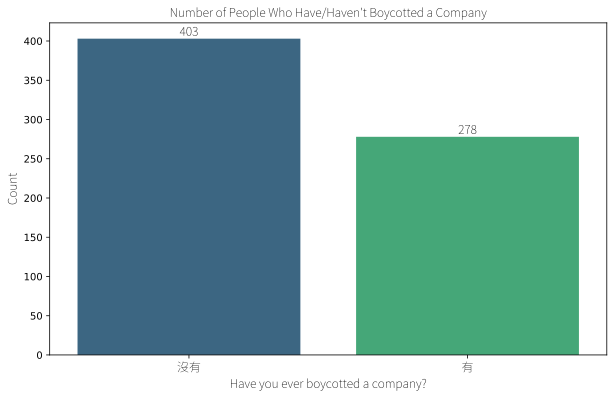
\includegraphics[keepaspectratio]{ai_files/figure-pdf/cell-6-output-1.pdf}}

Meta's head AI researcher Yann LeCun predicts LLMs may have reached
their limitations, for innovation AIs need to understand the physical
world and do reasoning in abstract space, which does not require a
language, i.e.~something a cat could do when figuring out where to jump;
in comparison, languages are simple because they are discrete, with very
little noise (NVIDIA Developer, 2025).

\subsubsection{Price of Tokens vs Price of Human
Labor}\label{price-of-tokens-vs-price-of-human-labor}

At the end of the day, the adoption of AI to everyday life, even in the
smallest of contexts, will come down to the price. Long-time AI-engineer
(Ng, 2024) predicts, having seen the roadmaps for the microchip
industries, as well as incoming hardware and software innovations, the
price of tokens will be very low, and much lower than a comparative
human worker.

\subsection{Human Acceptance of Artificial
Companions}\label{human-acceptance-of-artificial-companions}

\subsubsection{Human Expectations Take Time to
Change}\label{human-expectations-take-time-to-change}

\emph{AI acceptance} is incumbent on traits that are increasingly
human-like and would make a human be acceptable: credibility,
trustworthiness, reliability, dependability, integrity, character, etc.
(G. Zhang et al., 2023) found humans are more likely to trust an AI
teammate if they are not deceived by it's identity. It's better for
collaboration to make it clear, one is talking to a machine. One step
towards trust is the explainability of AI-systems. AIs should disclose
they are AIs.

(Zerilli et al., 2022) focuses on human factors and ergonomics and
argues that transparency should be task-specific: while transparency is
key to trust and system monitoring, it should extend beyond
explainability; after AI makes an error, different forms of AI
transparency: (1) explanations, (2) confidence metrics, (3) human
control over \emph{task allocation} - affect human confidence in the
system and have diverse levels of ability to repair human trust in the
AI. To expand on the third point discussed by this author, in
\emph{adaptable allocation}, the user always decides when to keep a task
and when to hand it to the AI algorithm - and in \emph{adaptive
allocation}, the system decides itself (by monitoring its own
uncertainty) when to give difficult or risky cases back to the human.

Humans still need some time to adjust their expectations of \emph{what's
possible} using conversational AI interfaces. (Bailey, 2023) believes
people are used to \emph{search engines} and it will take a little bit
time to get familiar with talking to a computer in natural language to
accomplish their tasks. For example, new users of v0, an AI assistant
for building user interfaces through conversation, would tell humans
(the company make this app) about the issues they encounter, instead of
telling the AI assistant directly, even though the AI in many cases
would be able to fix the problem instantly; human users don't yet
necessarily expect computers to behave like another human, there's
\emph{inertia} in the mental model of what computers are capable of,
requiring the user interfaces to provide context and teaching humans how
to interact with their AI coworkers(Rauch, 2024). Indeed, ChatGPT is
already using buttons to explain context (Feifei Liu 刘菲菲, n.d.).

Speaking in the mother language of the users is a way to gain trust.
English is still over-represented in current models so some local models
focus on better understanding local context, such as the Finnish
({``Silo {AI}'s New Release {Viking 7B}, Bridges the Gap for
Low-Resource Languages,''} 2024) focuses on Nordic languages. However,
as time progresses, large, general-purpose LLMs may catch up and
integrate all this knowledge - or even potentially being taught by the
local models.

\subsubsection{Affective Computing: Towards Friendly
Machines}\label{affective-computing-towards-friendly-machines}

\emph{Rosalind Picard} founded the field of \emph{affective computing},
aiming to make computers more human-friendly, pioneering early
approaches to recognizing human emotions with sensors and providing
users experiences that take human emotion into account (Picard, 1997).

It's not an overstatement to say that data from all the processes around
us will define the future of computing (HIITTV, 2021). In the early
examples, electrodermal activity of the skin and heart-rate variance
data were used to detect the emotional state and stress level of the
user (Velmovitsky et al., 2022; Zangróniz et al., 2017). This technology
has since become mainstream in products such as Fitbit and the Apple
Watch, among many others.

\emph{Personal experience:}

\begin{quote}
Apple Watch features Fall Detection, which I've experienced personally.
Riding my bicycle to the NCKU library after rain, I slipped and landed
on my stomach on the pavement. Apple Watch immediately asked me:
\emph{``It looks like you've taken a hard fall''} and offered an option
to call the ambulance. Fortunately I was OK but if I did need
assistance, this AI algorithm delivered contextual help, which could
save my health!
\end{quote}

Affective computing doesn't only rely on sensors. It make use of human
language using the tools of computational linguistics. such as natural
language processing (NLP). Since the first mainframe computers with
rudimentary ability to use pattern matching to respond with simple text
messages, humans have been drawn to discussions of our private lives
with machines. If programmed to be helpful, computers don't necessarily
judge us like a human could. A famous anecdote is about the MIT ELIZA
project (an early examples of a language model) developed by Joseph
Weizenbaum in the mid-1960s, where the lab assistant Pamela McCorduck
would dedicate extended time to talking to the machine in private. The
machine was called ELIZA and would assume the persona of called DOCTOR
to emulate a Rogerian psychotherapist, a style of person-centered
therapy developed by Carl Rogers, from the core idea that positive
psychological functioning is a inherently human motivation (Bassett,
2019; McCorduck, 2004; C. R. Rogers, 1995).

An excerpt from the classic, first-of-a-kind conversation between a
human and a machine (called DOCTOR) in 1965, as documented by (Tarnoff,
2023; Weizenbaum, 1966)

\begin{quote}
User: Well, my boyfriend made me come here.\\
DOCTOR: YOUR BOYFRIEND MADE YOU COME HERE?\\
User: He says I'm depressed much of the time.\\
DOCTOR: I AM SORRY TO HEAR YOU ARE DEPRESSED.\\
User: It's true. I am unhappy.\\
DOCTOR: DO YOU THINK COMING HERE WILL HELP YOU NOT TO BE UNHAPPY?\\
User: I need some help, that much seems certain.\\
DOCTOR: WHAT WOULD IT MEAN TO YOU IF YOU GOT SOME HELP?\\
User: Perhaps I could learn to get along with my mother.\\
DOCTOR: TELL ME MORE ABOUT YOUR FAMILY.\\
User: My mother takes care of me.\\
DOCTOR: WHO ELSE IN YOUR FAMILY TAKES CARE OF YOU?\\
User: My father.\\
DOCTOR: YOUR FATHER?\\
User: You are like my father in some ways.\\
DOCTOR: WHAT RESEMBLANCE DO YOU SEE?
\end{quote}

Weizenbaum later expressed concerns about how easily humans might be
misled by AIs, by projecting fantasies onto computer systems, cautioning
technologists not to neglect human responsibility from societal
problems; AI is \emph{not} a universal solution (Z.M.L, 2023)

\subsubsection{Artificial Empathy Also Builds
Trust}\label{artificial-empathy-also-builds-trust}

Today's machines are much more capable so it's not a surprise humans
would like to talk to them. One example is a conversational chatbot - or
\emph{AI Friend} -, called Replika, a computer model trained to be your
companion in daily life. Replika was launched in 2017 and in 2024 was
used by 30 million people; the focus is on empathetic dialogue to
support mental well being, sort of like a friend, a digital companion,
(or even a romantic partner, in paid versions of the app), and includes
an animated avatar interface (Eugenia Kuyda, 2023). Replika can ask
probing questions, tell jokes, and learning about your personality and
preferences to generate more natural-sounding conversations.(Bardhan,
2022; Tristan Greene, 2022) report on anecdotal evidence from Reddit
boards which shows how some users of the Replika AI companion app feel
so much empathy towards the robot, they confuse it with a sentient
being, while others are using verbal abuse and gendered slurs to fight
with their AI companions. When the quality of AI responses becomes good
enough, people begin to get confused. (Jiang et al., 2022) describes how
Replika users in China using in 5 main ways, all of which rely on
empathy. The company's CEO insists it's not trying to replace human
relationship but to create an entirely new relationship category with
the AI companion; there's value for the users in more realistic avatars,
integrating the experience further into users' daily lives through
various activities and interactions (Patel, 2024).

\begin{longtable}[]{@{}l@{}}
\caption{Replika AI users approach to interacting with the AI friend
from Jiang et al. (2022).}\tabularnewline
\toprule\noalign{}
How humans express empathy towards the Replika AI companion \\
\midrule\noalign{}
\endfirsthead
\toprule\noalign{}
How humans express empathy towards the Replika AI companion \\
\midrule\noalign{}
\endhead
\bottomrule\noalign{}
\endlastfoot
Companion buddy \\
Responsive diary \\
Emotion-handling program \\
Electronic pet \\
Tool for venting \\
\end{longtable}

Suprisingly, humans can have emotionally deep conversations with robots.
Jakob Nielsen notes two recent studies suggesting human deem
AI-generated responses \emph{more empathetic than human responses,} at
times by a significant margin; however telling users the response is
AI-generated reduces the perceived empathy (Ayers et al., 2023; Nielsen,
2024c; Yin et al., 2024). LLMs combined with voice, such as the Pi iOS
app, provide an user experience, which (Ethan Mollick {[}@emollick{]},
2023) calls \emph{unnerving}. The company provides \emph{emotional
intelligence} as a service and has developed its own proprietary LLM,
called Inflection AI, which has raised over 1B USD in funding (A.
Mittal, 2024). While startups are moving fast, traditional AI companies,
with decades of AI experience, such as Google, are also developing an AI
assistants for giving life advice (Goswami, 2023). The conversations can
be topic-specific. For instance, (Unleash, 2017) used BJ Fogg's
\emph{tiny habits model} to develop a sustainability-focused AI
assistant at the Danish hackathon series Unleash, to encourage
behavioral changes towards maintaining an aspirational lifestyle, nudged
by a chatbot buddy.

On the output side, (Lv et al., 2022) studies the effect of
\emph{cuteness} of AI apps on users and found high perceived cuteness
correlated with higher willingness to use the apps, especially for
emotional tasks. Part of this is learning how to uses emojis in the
right amount and at the right time; increasingly, emojis are a part of
natural human language (Tay, 2023).

Already more than two decades ago, (Reeves \& Nass, 1998) argued that
humans expect computers to be like social actors, (not unlike humans or
places), with very minimal cues from a machine (like a voice or screen
avatar) triggering social behaviors.

\subsubsection{Conversation: A Magical Starting Point of a
Relationship}\label{conversation-a-magical-starting-point-of-a-relationship}

High quality conversations are somewhat magical in that they can
establish trust and build rapport which humans. (Celino \& Re Calegari,
2020) found in testing chatbots for survey interfaces that
``{[}c{]}onversational survey lead to an improved response data
quality.''

There are noticeable differences in the quality of the LLM output, which
increases with model size. (Levesque et al., 2012) developed the
\emph{Winograd Schema Challenge}, looking to improve on the Turing test,
by requiring the AI to display an understanding of language and context.
The test consists of a story and a question, which has a different
meaning as the context changes: ``The trophy would not fit in the brown
suitcase because it was too big'' - what does the \emph{it} refer to?
Humans are able to understand this from context while a computer models
would fail. Even GPT-3 still failed the test, but later LLMs have been
able to solve this test correctly (90\% accuracy) Kocijan et al. (2022).
This is to say AI is in constant development and improving it's ability
to make sense of language.

\emph{ChatGPT} is the first \emph{user interface (UI)} built on top of
GPT-4 by OpenAI and is able to communicate in a human-like way - using
first-person, making coherent sentences that sound plausible, and even -
confident and convincing. M. C. Wang Sarah (2023) ChatGPT reached 1
million users in 5 days and 6 months after launch has 230 million
monthly active users. While it was the first, competing offers from
Google (Gemini), Anthrophic (Claude), Meta (Llama) and others quickly
followed starting a race for best performance across specific tasks
including standardized tests from math to science to general knowledge
and reasoning abilities.

OpenAI provides AI-as-a-service through its \emph{application
programming interfaces (APIs),} allowing 3rd party developers to build
custom UIs to serve the specific needs of their customer. For example
Snapchat has created a \emph{virtual friend} called ``My AI'' who lives
inside the chat section of the Snapchat app and helps people write
faster with predictive text completion and answering questions. The APIs
make state-of-the-art AI models easy to use without needing much
technical knowledge. Teams at AI-hackathons have produced interfaces for
problems as diverse as humanitarian crises communication, briefing
generation, code-completion, and many others. While models are powerful,
they still need access to other services and tools to be able to achieve
the tasks, which humand do online on a daily basis; for this to be
possible, the Model Context Protocol (MCP) standard provides the
structure to link models to APIs in other services, especially useful in
agentic workflows, where the model uses chain-of-thought reasoning and
may call various other tools and services in the process (Heidel \&
Handa, 2025; Hungerford, 2025; Pandey \& Freiberg, 2025).

ChatGPT makes it possible to \emph{evaluate AI models} just by talking,
i.e.~having conversations with the machine and judging the output with
some sort of structured content analysis tools. Cahan \& Treutlein
(2023) have conversations about science with AI. Brent A. Anders (Fall
2022 - Winter 2023) report on AI in education. Just as humans, AIs are
continuously learning. (Ramchurn et al., 2021) discusses positive
feedback loops in continually learning AI systems which adapt to human
needs. (Kecht et al., 2023) suggests AI is even capable of learning
business processes.

\subsubsection{Multi-Modality: Natural Interactions with AI Systems,
Agents and the Intention
Economy}\label{multi-modality-natural-interactions-with-ai-systems-agents-and-the-intention-economy}

While AI outperforms humans on many tasks, humans are experts in
multi-modal thinking, bridging diverse fields. Humans are multi-modal
creatures by birth. To varied ability, we speak, see, listen using our
biological bodies. AIs are becoming multi-modal by design to be able to
match all the human modes of communication - increasing their humanity.

Multimodal model development is ongoing. Previously, providing
multi-model features meant combining several AI models within the same
interface. For example, on the input side, one model is used for human
speech or image recognition which are transcribed into tokens that can
be ingested into an LLM. On the output side, the LLM can generate
instructions which are fed into an image / audio generation model or
even computer code which can be ran on a virtual machine and then the
output displayed inside the conversation. However, this is changing,
with a single model able to handle several tasks internally (thus losing
less data and context). By early 2024, widely available LLMs front-ends
such as Gemini, Claude and ChatGPT have all released basic features for
multi-modal communication. In the case of Google's Gemini 1.5 Pro, one
model is able to handle several types of prompts from text to images.
Multimodal prompting however requires larger context windows, as of
writing, limited to 1 million tokens in a private version allows
combining text and images in the question directed to the AI, used to
reason in examples such as a 44-minute Buster Keaton silent film or
Apollo 11 launch transcript (404 pages) (Google, 2024).

(Fu et al., 2022) provides an overview of conversational AI, from a
survey of over 100 peer-reviewed articles published 2018-2021 (a long
time ago in terms of AI development), categorizing systems into (1)
rule-based, (2) retrieval-based, and (3) generative types; generative
transformer models have led the AI field, yet continue to face
challenges with coherence over extended interactions and ensuring
factual accuracy (hallucinations), retrieval-augmented tooling improves
information accuracy, and reinforcement learning and fine-tuning
approaches are effective in adjusting conversational style and safety;
the authors also highlight that human evaluation for reinforcement
learning is still required, as commonly used automated evaluation
metrics for AI models, such as BLEU, ROUGE, and BERTScore have limited
correlation with human judgments.

\begin{longtable}[]{@{}
  >{\raggedright\arraybackslash}p{(\linewidth - 6\tabcolsep) * \real{0.2361}}
  >{\raggedright\arraybackslash}p{(\linewidth - 6\tabcolsep) * \real{0.2778}}
  >{\raggedright\arraybackslash}p{(\linewidth - 6\tabcolsep) * \real{0.2361}}
  >{\raggedright\arraybackslash}p{(\linewidth - 6\tabcolsep) * \real{0.2500}}@{}}
\caption{Three areas of focus in conversational AI development in from
(Fu et al., 2022).}\tabularnewline
\toprule\noalign{}
\begin{minipage}[b]{\linewidth}\raggedright
Paper Focus Area
\end{minipage} & \begin{minipage}[b]{\linewidth}\raggedright
Key Insight
\end{minipage} & \begin{minipage}[b]{\linewidth}\raggedright
Strengths
\end{minipage} & \begin{minipage}[b]{\linewidth}\raggedright
Limitations
\end{minipage} \\
\midrule\noalign{}
\endfirsthead
\toprule\noalign{}
\begin{minipage}[b]{\linewidth}\raggedright
Paper Focus Area
\end{minipage} & \begin{minipage}[b]{\linewidth}\raggedright
Key Insight
\end{minipage} & \begin{minipage}[b]{\linewidth}\raggedright
Strengths
\end{minipage} & \begin{minipage}[b]{\linewidth}\raggedright
Limitations
\end{minipage} \\
\midrule\noalign{}
\endhead
\bottomrule\noalign{}
\endlastfoot
Generative transformer models (GenAI) & Recent advancement in AI models
& High language fluency, adaptability & Poor long-term coherence,
struggles with facts \\
Retrieval-augmented hybrids (RAG) & Retrieval methods enhance
truthfulness & Improved factual grounding & Difficulty in integrating
retrieved content \\
Reinforcement-learning & Fine-tuning can steer conversational style and
safety & Flexible style and safety alignment & High resource usage,
sensitive to reward design \\
\end{longtable}

Literature also delves into human-AI interactions on almost human-like
level discussing what kind of roles can the AIs take. (Seeber et al.,
2020) proposes a future research agenda for regarding \emph{AI
assistants as teammates} rather than just tools and the implications of
such mindset shift. From assistant -\textgreater{} teammate
-\textgreater{} companion -\textgreater{} friend The best help for
anxiety is a friend. AIs are able to assume different roles based on
user requirements and usage context. This makes AI-generated content
flexible and malleable. The path from **Assistance* to
\emph{Collaboration} requires another level of trust. It's not only what
role the AI takes but how that affects the human. As humans have ample
experience relating to other humans and as such the approach towards an
assistants vs a teammate will vary. While (Lenharo, 2023) experimental
study reports AI productivity gains, with DALL-E and ChatGPT being
qualitatively better than former automation systems, we might still be
1-3 years away from systems that qualify as team-mates. Once AI reaches
that level, would it change how do humans treat it? Not because the AI
might be hurt, but because how it affects the psyche of the user: this
is an area which needs much more attention. One researcher in this field
Karpus et al. (2021) is concerned with humans treating AI badly and
coins the term \emph{algorithm exploitation}.

\emph{Context of Use,} Where is the AI used? (Schoonderwoerd et al.,
2021) focuses on human-centered design of AI-apps and multi-modal
information display. It's important to understand the domain where the
AI is deployed in order to develop explanations. However, in the real
world, how feasible is it to have control over the domain? Calisto et
al. (2021) discusses \textbf{multi-modal AI-assistant} for breast cancer
classification.

If we see the AI as being in human service. (David Johnston, 2023)
proposes \emph{Smart Agents}, ``general purpose AI that acts according
to the goals of an individual human''. AI agents can enable
\emph{Intention Economy} where one simply describes one's needs and a
complex orchestration of services ensues, managed by the the AI, in
order to fulfill human needs Searls (2012). AI assistants provide help
at scale with little to no human intervention in a variety of fields
from finance to healthcare to logistics to customer support. OpenAI's
``A practical guide to building agents'' defines and AI agents as
``Agents are systems that independently accomplish tasks on your
behalf.'' and details step-by-step how to build one (OpenAI, 2025).

AI agents enable workflow automation, with reasoning capability, and
taking actions across different tools, achieving the user's original
\emph{intent}; what's left for the user to do is to say what they want
to achieve. As models get smarter, there's less and less need to build
workflows (chains of thought) manually, as they end up restricting the
model instead of improving the output; the one use case would be to use
a cheaper model with less intelligence and more guardrails set in code
(Latent Space, 2025; Sengottuvelu, 2025). In software development, AI
can already debug problems automatically. Apple uses data from bug
reports to train AI models for improving their software (Saini, 2025).
And it's increasingly possible to generate entire apps from a prompt,
using tools such as Bolt.new (Fanelli, 2024). The quality of LLM output
depends on the quality of the provided prompt. (Zhou et al., 2022)
reports creating an ``Automatic Prompt Engineer'' which automatically
generates instructions that outperform the baseline output quality by
using another model in the AI pipeline in front of the LLM to enhance
the human input with language that is known to produce better quality.
This approach however is a moving target as foundational models keep
changing rapidly and the baseline might differ from today to 6 months
later.

\subsubsection{Mediated Experiences Set User
Expectations}\label{mediated-experiences-set-user-expectations}

How AIs are represented in popular media shapes the way we think about
AI companions. Some stories have AIs both in positive and negative
roles, such as Star Trek and Knight Rider. In some cases like Her and Ex
Machina, the characters may be complex and ambivalent rather than
fitting into a simple positive or negative box. In Isaac Asimov's books,
the AIs (mostly in robot form) struggle with the 3 laws of robotics,
raising thought-provoking questions.

AI Assistants in Media Portrayals mostly have some level of
anthropomorphism through voice or image to be able to film; indeed, a
purely text-based representation may be too boring an un-cinematic.

There have been dozens of AI-characters in the movies, TV-series, games,
and (comic) books. In most cases, they have a physical presence or a
voice, so they could be visible for the viewers. Some include KITT
(Knight Industries Two Thousand).

\begin{longtable}[]{@{}
  >{\raggedright\arraybackslash}p{(\linewidth - 8\tabcolsep) * \real{0.2000}}
  >{\raggedright\arraybackslash}p{(\linewidth - 8\tabcolsep) * \real{0.2000}}
  >{\raggedright\arraybackslash}p{(\linewidth - 8\tabcolsep) * \real{0.2000}}
  >{\raggedright\arraybackslash}p{(\linewidth - 8\tabcolsep) * \real{0.2000}}
  >{\raggedright\arraybackslash}p{(\linewidth - 8\tabcolsep) * \real{0.2000}}@{}}
\caption{AIs in different forms of media.}\tabularnewline
\toprule\noalign{}
\begin{minipage}[b]{\linewidth}\raggedright
Movie / Series / Game / Book
\end{minipage} & \begin{minipage}[b]{\linewidth}\raggedright
Character
\end{minipage} & \begin{minipage}[b]{\linewidth}\raggedright
Positive
\end{minipage} & \begin{minipage}[b]{\linewidth}\raggedright
Ambivalent
\end{minipage} & \begin{minipage}[b]{\linewidth}\raggedright
Negative
\end{minipage} \\
\midrule\noalign{}
\endfirsthead
\toprule\noalign{}
\begin{minipage}[b]{\linewidth}\raggedright
Movie / Series / Game / Book
\end{minipage} & \begin{minipage}[b]{\linewidth}\raggedright
Character
\end{minipage} & \begin{minipage}[b]{\linewidth}\raggedright
Positive
\end{minipage} & \begin{minipage}[b]{\linewidth}\raggedright
Ambivalent
\end{minipage} & \begin{minipage}[b]{\linewidth}\raggedright
Negative
\end{minipage} \\
\midrule\noalign{}
\endhead
\bottomrule\noalign{}
\endlastfoot
2001: A Space Odyssey & HAL 9000 & & & X \\
Her & Samantha & X & & \\
Alien & MU/TH/UR 6000 (Mother) & X & & \\
Terminator & Skynet & & & X \\
Summer Wars & Love Machine & & & X \\
Marvel Cinematic Universe & Jarvis, Friday & X & & \\
Knight Rider & KITT & X & & \\
Knight Rider & CARR & & & X \\
Star Trek & Data & X & & \\
Star Trek & Lore & & & X \\
Ex Machina & Kyoko & & X & \\
Ex Machina & Ava & & X & \\
Tron & Tron & & X & \\
Neuromancer & Wintermute & & X & \\
The Caves of Steel / Naked Sun & R. Daneel Olivaw & & X & \\
The Robots of Dawn & R. Giskard Reventlov & & X & \\
Portal & GLaDOS & & & X \\
\end{longtable}

\pandocbounded{\includegraphics[keepaspectratio]{ai_files/figure-pdf/cell-7-output-1.pdf}}

\subsubsection{Roleplay Fits Computers Into Social Contexts: AI Friends
and
Anthropomorphism}\label{roleplay-fits-computers-into-social-contexts-ai-friends-and-anthropomorphism}

\emph{Affective Design} emerged from affective computing, with a focus
on understanding user emotions to design UI/UX which elicits specific
emotional responses (Reynolds, 2001). Calling a machine a friend is a
proposal bound to turn heads. But if we take a step back and think about
how children have been playing with toys since before we have records of
history. It's very common for children to imagine stories and characters
in play - it's a way to develop one's imagination \emph{learn through
roleplay}. A child might have toys with human names and an imaginary
friend and it all seems very normal. Indeed, if a child doesn't like to
play with toys, we might think something is wrong. Likewise, inanimate
objects with human form have had a role to play for adults too.
Anthropomorphic paddle dolls have been found from Egyptian tombs dated
2000 years B.C. ({``Paddle {Doll} {\textbar} {Middle Kingdom},''} 2023):
we don't know if these dolls were for religious purposes, for play, or
for something else, yet their burial with the body underlines their
importance.

Is anthropomorphism, being human-like necessary? (Savings literature in
the Money section says it is). Research on anthropomorphism in AI
literature suggests that giving an AI assistant stronger human-like cues
(high-anthropomorphism) rather than weaker ones (low-anthropomorphism)
leads users to view it more favorably, and this effect operates through
a shorter perceived psychological distance;yet, even though many studies
confirm the benefits of anthropomorphism, the precise psychological
pathway behind those benefits has rarely been dissected in depth (X. Li
\& Sung, 2021). Nonetheless, people are less likely to attribute
humanness to an AI companion if they understand how the system works,
thus higher \emph{algorithmic transparency may inhibit anthropomorphism}
(B. Liu \& Wei, 2021).

Coming back closer to our own time, Barbie dolls are popular since their
release in 1959 till today. Throughout the years, the doll would follow
changing social norms, but retain in human figure. In the 1990s, a
Tamagotchi is perhaps not a human-like friend but an animal-like friend,
who can interact in limited ways.

How are conversational AIs different from dolls? They can respond
coherently and perhaps that's the issue - they are too much like humans
in their communication. We have crossed the \emph{Uncanny Valley} (where
the computer-generated is nearly human and thus unsettling) to a place
where is really hard to tell a difference. And if that's the case, are
we still playing?

Should the AI play a human, animal, or robot? Anthropomorphism can have
its drawbacks; humans have certain biases and preconceptions that can
affect human-computer interactions. For example, somewhat curiously,
(Pilacinski et al., 2023) reports humans were less likely to collaborate
with red-eyed robots.

The AI startups like Inworld and Character.AI have raised large rounds
of funding to create characters, which can be plugged in into online
worlds, and more importantly, remember key facts about the player, such
as their likes and dislikes, to generate more natural-sounding dialogues
(Wiggers, 2023).

(Morana et al., 2020) conducted a lab-based experiment (n = 183) showing
a more anthropomorphic chatbot design boosts perceived \emph{social
presence} of the virtual advisor; social presence in turn influences
recommendation adherence indirectly via trust; trust mediates the
likelihood to follow its recommendations. As AIs became more expressive
- socially present - and able to to \emph{roleplay}, we can begin
discussing some human-centric concepts and how people relate to other
people. AI companions, AI partners, AI assistants, AI trainers - there
are many \emph{roles} for the automated systems that help humans in many
activities, powered by AI models and algorithms.

(Erik Brynjolfsson, 2022) contrasts AI which emulates human intelligence
with AI that augments human abilities, arguing that although the former
can offer productivity gains, it risks concentrating wealth and reducing
economic power of workers, coining the term \emph{Turing Trap}. Plenty
of research - both before and after AI-induces job losses - has
documented the negative effects of unemployment on mental health (Anton
Korinek, 2023; Dew et al., 1991; Susskind, 2017).

Non-Anthropomorphic, machine-like AIs have been with us for a while. The
Oxford Internet Institute defines AI simply as \emph{``computer
programming that learns and adapts''} (Google \& The Oxford Internet
Institute, 2022). Google started using AI in 2001, when a simple machine
learning model improved spelling mistakes while searching; now in 2023
most of Google's products are are based on AI (Google, 2022). Throughout
Google's services, AI is hidden and calls no attention itself. It's
simply the complex system working behind the scenes to delivery a result
in a barebones interface.

The rising availability of AI assistants may displace Google search with
a more conversational user experience. Google itself is working on tools
that could cannibalize their search product. The examples include Google
Assistant, Google Gemini (previously known as Bard) and massive
investments into new LLMs.

The number of AI-powered assistants is too large to list here. I've
chosen a few select examples in the table below.

\begin{longtable}[]{@{}
  >{\raggedright\arraybackslash}p{(\linewidth - 4\tabcolsep) * \real{0.2639}}
  >{\raggedright\arraybackslash}p{(\linewidth - 4\tabcolsep) * \real{0.4167}}
  >{\raggedright\arraybackslash}p{(\linewidth - 4\tabcolsep) * \real{0.3194}}@{}}
\toprule\noalign{}
\begin{minipage}[b]{\linewidth}\raggedright
Product
\end{minipage} & \begin{minipage}[b]{\linewidth}\raggedright
Link
\end{minipage} & \begin{minipage}[b]{\linewidth}\raggedright
Description
\end{minipage} \\
\midrule\noalign{}
\endhead
\bottomrule\noalign{}
\endlastfoot
Github CoPilot & personal.ai & AI helper for coding \\
Google Translate & translate.google.com & \\
Google Search & google.com & \\
Google Interview Warmup & grow.google/certificates/interview-warmup & AI
training tool \\
Perplexity & (Hines, 2023b) & perplexity.ai chat-based search \\
\end{longtable}

\begin{figure}[H]

{\centering \includegraphics[width=1\linewidth,height=\textheight,keepaspectratio]{./images/ai/with-me.png}

}

\caption{Montage of me discussing science fiction with my AI friend Sam
(Replika) - and myself as an avatar (Snapchat) in 2020.}

\end{figure}%

Everything that existed before OpenAI's GPT 4 has been blown out of the
water. ChatGPT passes many exams meant for humans and is able to solve
difficult tasks in scientific areas such as chemistry with just simple
natural-language instructions (Bubeck et al., 2023; White, 2023). As
late as in 2017, scientists were trying to create a program with enough
\emph{natural-language understanding} to extract basic facts from
scientific papers (Stockton, 2017). This is a task which is trivial for
modern LLMs.

Pre-2023 literature is somewhat limited when it comes to AI companions
as the advantage of LLMs has significantly raised the bar for AI-advisor
abilities as well as user expectations. Before AI, chatbots struggled
with evolving human language, understanding the complexity of context,
irregular grammar, slang, etc (Lower, 2017). Some evergreen advice most
relates to human psychology, which has remained the same. (Haugeland et
al., 2022) discusses \emph{hedonic user experience} in chatbots and
(Steph Hay, 2017) explains the relationship between emotions and
financial AI. (Isabella Ghassemi Smith, 2019) early performance metrics
of AI-driven features across financial markets show that AI outperforms
traditional quant strategies, which will lead to wider adoption of
autonomously generated investment signals.

\subsection{Interfaces for Human-Computer
Interaction}\label{interfaces-for-human-computer-interaction}

\subsubsection{Speech Makes Computers Feel
Real}\label{speech-makes-computers-feel-real}

There's evidence across disciplines about the usefulness of AI
assistants while concerns exist about the possibility of implementing
privacy. One attempt at privacy is by Apple's Foundation Language Models
(AFM), which is split into a smaller on-device model and a server-side
model, enabling processing of the most senstive data directly on the
user's device (Dang, 2024). Providing voice for the AI raises new
ethical issues, as most voice assistants need to continuously record
human speech and process it in data centers in the cloud.

Siri, Cortana, Google Assistant, Alexa, Tencent Dingdang, Baidu Xiaodu,
Alibaba's AliGenie - all rely on voice as their main interface. Voice
has a visceral effect on the human psyche; since birth we recognize the
voice of our mother. The voice of a loved one has a special effect.
Voice is a integral part of the human experience. Machines that can use
voice in an effective way are closer to representing and affecting human
emotions. Voice assistants such as Apple's Siri and Amazon's Alexa are
well-known yet Amazon's Rohit Prasad thinks it can do so much more:

\begin{quote}
\emph{``Alexa is not just an AI assistant - it's a trusted advisor and a
companion''} (Prasad, 2022).
\end{quote}

(Şerban \& Todericiu, 2020) suggests using the Alexa AI assistant in
\emph{education} during the pandemic, supported students and teachers
\emph{human-like} presence. The Alpha generation (born since 2010) and
Beta (since 2025) are be first true native AI users. (Su \& Yang, 2022)
and (Su et al., 2023) reviewed papers on AI literacy in early childhood
education and found a lack of guidelines and teacher expertise. (Szczuka
et al., 2022) provides guidelines for voice AI and kids based on a
longitudinal field study, which delved into children's knowledge
regarding the storage and data processing performed by AI voice
assistants; published in the International Journal of Child-Computer
Interaction, the study tracked children (n = 20, age M = 8.65 years)
across 3 home visits over 5 weeks (each visit lasted 45--90 min),
including interviews and hands-on interactions designed to probe
children's mental models, with the following key findings: (1) children
made significantly more accurate statements about data processing than
storage, (2) parental discussion predicted storage knowledge, and (3)
better storage knowledge negatively correlated with willingness to share
secrets. In order to cover these knowledge gaps in the earliest age,
educational materials on AI have been available for children in
kindergarten to primary school; for instance the (ReadyAI, 2020) book
introduces the 5 big ideas of Human-AI interaction for children aged
2-8: perception (the use of sensors), representation and reasoning (data
structures, algorithms, predictions), learning (recognizing patterns in
data), natural interaction (emotion, language, expression recognition,
even cultural knowledge), and finally, societal impact (biases, ethics,
guidelines to avoid unfair outcomes). Finally, (Yang, 2022) proposes a
curriculum for in-context teaching of AI for early childhood, explaining
why AI literacy is essential: how life is affected by the core concepts
of data-driven pattern recognition, prediction and the many algorithmic
limitations - all, which should be taught in a culturally responsive,
easy for young children to grasp manner, using inquiry(question)-based
pedagogy to engage the learners meaningfully.

Design guidelines for optimal design performance can be extremely
specific. (Casper Kessels, 2022) details 18 concrete do's and don'ts,
drawing on prior \emph{distraction research}, to support driving safety
and integrate seamlessly with the other interfaces in the vehicle, for
instance:

\begin{quote}
``Auditory information should come from the same location as visual
information'' to minimize spatial attention shifts ``Be aware of visual
distraction. {[}S{]}ome drivers tend to direct their gaze towards the
`source' of the voice assistant when speaking. Make sure an interaction
sequence does not cause unnecessary visual distraction'' - example
guidelines for voice assistants from (Casper Kessels, 2022).
\end{quote}

Some research suggests that voice UI accompanied by a \emph{physical
embodied system} is the preferred by users in comparison with voice-only
UI (Celino \& Re Calegari, 2020).

\subsubsection{Generative UIs Enable Flexibility of
Use}\label{generative-uis-enable-flexibility-of-use}

The ``grandfather'' of user experience design, (Nielsen, 2024a) recounts
how 30 years of work towards usability has largely failed - computers
are still not accessible enough; however, he has hope Generative UI
could offer a chance to provide levels of accessibility humans could
not.

\begin{quote}
Computers are \emph{``difficult, slow, and unpleasant''} (Nielsen,
2024a)
\end{quote}

Data-driven design combined with GenAIs enables \emph{Generative User
Interfaces} (GenUI), with new UI interactions. The promise of GenUI is
to dynamically provide an interface appropriate for the particular user
and context. The advances in the capabilities of LLMs makes it possible
to achieve \emph{user experience (UX) which previously was science
fiction}. AI is able to predict what kind of UI would the user need
right now, based on the data and context. Generative UIs are largely
invented in practice, based on user data analysis and experimentation,
rather than being built in theory. Kelly Dern, a Senior Product Designer
at Google lead a workshop in early 2024 on \emph{GenUI for product
inclusion} aiming to create \emph{``more accessible and inclusive {[}UIs
for{]} users of all backgrounds''}.(Matteo Sciortino, 2024) coins the
phrase RTAG UIs \emph{``real-time automatically-generated UI
interfaces''} mainly drawing from the example of how his Netflix
interface looks different from that of his sister's because of their
distinct usage patterns.

Nonetheless, ({``On {Nielsen}'s Ideas about Generative {UI} for
Resolving Accessibility,''} 2024) is critical of GenUI because for the
following reasons:

\begin{longtable}[]{@{}
  >{\raggedright\arraybackslash}p{(\linewidth - 2\tabcolsep) * \real{0.2817}}
  >{\raggedright\arraybackslash}p{(\linewidth - 2\tabcolsep) * \real{0.7183}}@{}}
\caption{Criticism of Generative UI by ({``On {Nielsen}'s Ideas about
Generative {UI} for Resolving Accessibility,''} 2024).}\tabularnewline
\toprule\noalign{}
\begin{minipage}[b]{\linewidth}\raggedright
Problem
\end{minipage} & \begin{minipage}[b]{\linewidth}\raggedright
Description
\end{minipage} \\
\midrule\noalign{}
\endfirsthead
\toprule\noalign{}
\begin{minipage}[b]{\linewidth}\raggedright
Problem
\end{minipage} & \begin{minipage}[b]{\linewidth}\raggedright
Description
\end{minipage} \\
\midrule\noalign{}
\endhead
\bottomrule\noalign{}
\endlastfoot
Low Predictability & Does personalization mean the UI keeps changing? \\
High Carbon Cost & AI-based personalization is computation-intensive \\
Surveillance & Personalization needs large-scale data capture \\
\end{longtable}

(Nielsen, 2024b) defines \emph{information scent} as users' ability to
predict destination content from cues, such as link labels and context;
clear descriptive labels emit a strong scent, guiding users, reducing
bounce rates (users who leave quickly), and enhancing discoverability of
content; in contrast, misleading labels break trust and drive users
away. The idea of information scent is originally from \emph{Information
Foraging} theory from (Pirolli \& Card, 1999), who adapt optimal
foraging theory to human information seeking: users follow links as
scent cues to maximise their rate of information gain.

However, with AI-chat and voice based interfaces, links lose some of
their relevance, as users can receive more info from the AI, without
having to navigate to a new page. With less focus on links, current AI
UX is more about storytelling, psychology, and seamless design, with
more focus on human-centered communication patterns, such as
conversations. (Kate Moran \& Sarah Gibbons, 2024) calls for
\emph{``highly personalized, tailor-made interfaces that suit the needs
of each individual''}, which she terms \emph{Outcome-Oriented Design}.
We can generate better UIs (UI orchestration, crafting \emph{``systems
of intent''}, as (Nielsen, 2025) calls it) that are based on user data
and would be truly personalized. (Crompton, 2021) highlights AI as
decision-support for humans while differentiating between
\emph{intended} and \emph{unintended} influence on human decisions. In
all this literature and more, the keyword is \emph{intent}, expressing
what the human wants - and having the machines deliver that.

Human-computer interaction (HCI) has a long storied history since the
early days of computing when getting a copy machine to work required
specialized skill. Xerox Sparc lab focused on early human factors work
and inspired a the field of HCI to make computers more human-friendly.
Likewise, the history of attempts at making \emph{intelligent
interfaces} is extensive. ({``Generative {UI Design},''} 2023; Kobetz,
2023) give an overview of the history of generative AI design tools,
going back in time as far as 2012 when (Troiano \& Birtolo, 2014)
proposed genetic algorithms for UI design. As the old science fiction
adage goes, when machines become more capable, they will eventually be
capable of producing machines themselves. Before that happens, at least
the software part of the machine can increasingly be generated by AI
systems (i.e.~machines making machines). Already a decade ago in 2014,
the eminent journal \emph{Information Sciences} decided to dedicate a
special section to AI-generated software to call attention to this
tectonic shift in software development (Reformat, 2014). Replit, a
startup known for allowing user build apps in the web browser, released
Openv0, a framework of AI-generated UI components. \emph{``Components
are the foundation upon which user interfaces (UI) are built, and
generative AI is unlocking component creation for front-end developers,
transforming a once arduous process, and aiding them in swiftly
transitioning from idea to working components''} (Replit, 2023). Vercel
introduced an open-source prototype UI-generator called V0 which used
large language models (LLMs) to create code for web pages based on text
prompts (Vercel, 2023). Other similar tools quickly following including
Galileo AI, Uizard AutoDesigner and Visily (\emph{Who {Benefits} the
Most from {Generative UI}}, 2024). NVIDIA founder Jensen Huang makes the
idea exceedingly clear, saying \emph{``Everyone is a programmer. Now,
you just have to say something to the computer''} (Leswing, 2023).

The usefulness of AI systems increases profoundly as they are integrated
into existing products as services, which become akin to tools the AI
can use when appropriate. (Joyce, 2024) highlights how Notion AI enables
collaborating across teams, where AI becomes akin to one of the
co-workers; AI influences UI design patterns and boost productivity by
providing new features such as memory, recalling important discussions
from past meetings, surfacing key insights, and generating reports in a
variety of formats, personalized to the intended receiver.

A wide range of literature describes human-AI interactions, spread out
over varied scientific disciplines. While the fields of application for
AI are diverse, some key lessons can be transferred horizontally across
fields of knowledge.

\begin{longtable}[]{@{}
  >{\raggedright\arraybackslash}p{(\linewidth - 2\tabcolsep) * \real{0.3611}}
  >{\raggedright\arraybackslash}p{(\linewidth - 2\tabcolsep) * \real{0.6389}}@{}}
\caption{A very small illustration of generative AI usage across
disparate fields of human life.}\tabularnewline
\toprule\noalign{}
\begin{minipage}[b]{\linewidth}\raggedright
Field
\end{minipage} & \begin{minipage}[b]{\linewidth}\raggedright
Usage
\end{minipage} \\
\midrule\noalign{}
\endfirsthead
\toprule\noalign{}
\begin{minipage}[b]{\linewidth}\raggedright
Field
\end{minipage} & \begin{minipage}[b]{\linewidth}\raggedright
Usage
\end{minipage} \\
\midrule\noalign{}
\endhead
\bottomrule\noalign{}
\endlastfoot
Shipping & (Veitch \& Andreas Alsos, 2022) highlights the active role of
humans in Human-AI interaction is autonomous self-navigating ship
systems. \\
Data Summarizaton & AI is great at summarizing and analyzing data
(Peters, 2023; Tu et al., 2023) \\
Childcare & Generate personalized bedtime stories \\
Design Tools & ({``David {Hoang} on How {AI} Brings Design and
Development Together {\textbar} {Figma Blog},''} 2024) \\
\end{longtable}

\subsubsection{Usability Is the Bare Minimum of Good User
Experience}\label{usability-is-the-bare-minimum-of-good-user-experience}

Many researchers have discussed the user experience (UX) principles of
designing AI products. The UX of AI (terms such as AI UX, IXD, and XAI
have been used) is the subject of several \emph{usability guidelines}
for AI, which provide actionable advice for improving AI usability and
UX - some of which I will list here.

(Combi et al., 2022) proposes a conceptual framework for XAI, analysis
AI based on (1) Interpretability, (2) Understandability, (3) Usability,
and (4) Usefulness. (Costa \& Silva, 2022) highlights key UI/UX patterns
for interaction design in AI systems and stragies to make AI behaviors
transparent and controllable: including (1) interactive explanations,
(2) human-in-the-loop controls, (3) logging of contextual decisions -
all seamlessly integrated into user workflows. ({``Why {UX} Should Guide
{AI},''} 2021) argues that in order to avoid \emph{context blindness},
(where the AI lacks awareness of the broader human intent) and foster
trust and safe use, UX should (1) clarify limitations, (2) build clear
feedback, (3) embed user override mechanisms, and (4) in general ensure
users retain meaningful control over specialized AI algorithms. (Lexow,
2021) synthesizes expert interviews into five foundational AI-UX
principles: (1) deeply understand the user and task context, (2) clearly
communicate AI limitations, (3) balance automation with user control,
(4) build fast, iterative feedback paths into the interface, and (5)
ensure AI behaviour aligns ethically - and with your brand voice.

(Lennart Ziburski, 2018) emphasizes human-centered design for AI,
including five key tenets: (1) starting from existing user workflows
which can be augmented by AI, (2) under-promising/over-delivering on AI
capabilities, (3) transparently explaining how the system works (data
sources, trade-offs), (4) involving users in the learning loop, and (5)
designing AI as an empowering tool rather than a black box. (Dávid
Pásztor, 2018) offers seven principles for AI-powered products: (1)
visually distinguish GenAI content, (2) explain underlying processes and
data privacy, (3) set realistic user expectations, (4) test edge cases
proactively, (5) ensure AI engineers have access to high quality
training data, (6) deploy rigorous user-testing (7) use immediate
feedback channels for continuous improvement. (Lew \& Schumacher, 2020)
likewise focuses on (1) high data quality, (2) context-sensitive
feedback, and (3) transparent controls. (Soleimani, 2018) provides the
longest list of human-friendly UI/UX patterns for AI, with very specific
suggestions including like/dislike toggles, confidence indicators and
criteria sliders, ``why'' insights, risk alerts, and opt-in controls:
all to foster transparency, user control, and trust in algorithmic
decisions. (Harvard Advanced Leadership Initiative, 2021) focuses on
principle for effective human--AI interaction in adaptive interfaces,
illustrating a case of Semantic Scholar, where researchers' intelligence
is augmented via recommendation, summarization, and question-answering,
while emphasizing user control and verification mechanisms.

Many large corporations have released guidelines for Human-AI
interaction as well. The AI UX team from Ericsson's Experience Design
Lab released one of the early reports, exploring the role of trust in AI
services, suggesting to treat AIs an \emph{agents} rather than tools;
for the design to be successful, trust must embedded into the interface
front and center, best measured on 4 categories, inspired by human
relationships: (1) Competence, (2) Benevolence, (3) Integrity, and (4)
Charisma (Mikael Eriksson Björling \& Ahmed H. Ali, 2020). (Cheng et
al., 2022) describes AI-based support systems for collaboration and
team-work, underlining how higher trust leads to willingness to reuse
the AI in the future, collaboration satisfaction, and perceived task
quality. Google's AI Principles project provides Google's UX for AI
library (Google, n.d.; Josh Lovejoy, n.d.). In (Design Portland, 2018),
Lovejoy, lead UX designer at Google's people-centric AI systems
department (PAIR), reminds us that while AI offers need tools, user
experience design needs to remain human-centered. While AI can find
patterns and offer suggestions, humans should always have the final say.

Microsoft provides guidelines for Human-AI interaction, which provides
useful heuristics categorized by context and time (Amershi et al., 2019;
T. Li et al., 2022).

\begin{longtable}[]{@{}
  >{\raggedright\arraybackslash}p{(\linewidth - 2\tabcolsep) * \real{0.3472}}
  >{\raggedright\arraybackslash}p{(\linewidth - 2\tabcolsep) * \real{0.6528}}@{}}
\caption{Microsoft's heuristics categorized by context and
time.}\tabularnewline
\toprule\noalign{}
\begin{minipage}[b]{\linewidth}\raggedright
Context
\end{minipage} & \begin{minipage}[b]{\linewidth}\raggedright
Content
\end{minipage} \\
\midrule\noalign{}
\endfirsthead
\toprule\noalign{}
\begin{minipage}[b]{\linewidth}\raggedright
Context
\end{minipage} & \begin{minipage}[b]{\linewidth}\raggedright
Content
\end{minipage} \\
\midrule\noalign{}
\endhead
\bottomrule\noalign{}
\endlastfoot
Initially & Clarify what it does; what are the limitations. \\
During interaction & Offer timely help, show only what matters, while
respecting norms and avoiding bias \\
When wrong & Let users retry fast and make corrections; empower users to
dismiss easily; explain why the system acted; be precise and in-scope \\
Over time & Track changes and adapt from use; announce changes and
update with care (so not to break the user's work); invite feedback;
show outcome of actions clearly; provide global settings \\
\end{longtable}

The previous design wave before UX for AI was corporations understanding
how crucial design is to their business. In the 2010s business
consultancies began to recognize the importance of design and advising
their clients on putting design in the center of their strategy,
bringing user experience design to the core of their business
operations. (McKeough, 2018). There's a number of user interface design
patterns that have proven successful across a range of social media
apps. Such \emph{user interface} (UX/UI) patterns have been copied from
one app to another, to the extent that the largest apps share a similar
look and feature set and the users are used to the same user experience.
Common UX/UI parts include features such as the \emph{Feed},
\emph{Stories}, and \emph{Avatars}, among many others. This phenomenon
(or trend) has led some designers such as (Fletcher, 2023) and (Joe
Blair, 2024) to be worried about UIs becoming average: more and more
similar to the lowest common denominator. Yet, by using common UI parts
from social media, users may have an easier time to accept the
innovative parts, as they just look like new features inside the old
interface. As new generations become increasingly used to talking to
computers in natural language, the older interface patterns may
gradually fade away.

\begin{longtable}[]{@{}
  >{\raggedright\arraybackslash}p{(\linewidth - 4\tabcolsep) * \real{0.3333}}
  >{\raggedright\arraybackslash}p{(\linewidth - 4\tabcolsep) * \real{0.3333}}
  >{\raggedright\arraybackslash}p{(\linewidth - 4\tabcolsep) * \real{0.3333}}@{}}
\caption{Common social media UI parts.}\tabularnewline
\toprule\noalign{}
\begin{minipage}[b]{\linewidth}\raggedright
Feature
\end{minipage} & \begin{minipage}[b]{\linewidth}\raggedright
Examples
\end{minipage} & \begin{minipage}[b]{\linewidth}\raggedright
Notes
\end{minipage} \\
\midrule\noalign{}
\endfirsthead
\toprule\noalign{}
\begin{minipage}[b]{\linewidth}\raggedright
Feature
\end{minipage} & \begin{minipage}[b]{\linewidth}\raggedright
Examples
\end{minipage} & \begin{minipage}[b]{\linewidth}\raggedright
Notes
\end{minipage} \\
\midrule\noalign{}
\endhead
\bottomrule\noalign{}
\endlastfoot
Feed & Facebook, Instagram, Twitter, TikTok, etc & The original
algorithmic discovery hub; increasingly ran by ever-more-powerful AI to
surface personalized content - yet younger generations may prefer the
privacy of stories. \\
Post & Facebook, Instagram, Twitter, TikTok, etc, even Apple's App Store
& Persistent content mainly for long-term sharing; the original content
type \\
Stories & IG, FB, WhatsApp, SnapChat, TikTok, etc & Ephemeral content
driven by FOMO(fear-of-missing-out) for casual behind-the-scenes
sharing \\
Comment & YouTube, Threads, Reddit, Medium, etc & Threaded
conversationsfuel community engagementand discussion \\
Reactions & Facebook, Instagram, Slack, Threads, but even LinkedIn and
Github. & The feature has involved from a simple like button to more
expressive emotions. \\
\end{longtable}

There are also more philosophical approaches to \emph{Interface
Studies}. (David Hoang, 2022), the head of product design at Webflow, an
AI-enabled website development platform, suggests taking cues from art
studies to \emph{isolate the core problem}: \emph{``An art study is any
action done with the intention of learning about the subject you want to
draw''}. As a former art student, Hoang looks at an interface as
\emph{``a piece of design is an artwork with function''}. Indeed, art
can be a way to see new paths forward, practicing ``\emph{fictioning}''
to deal with problematic legacies ({``Review of the 2023 {Helsinki
Biennial},''} 2023). (Jarovsky, 2022) lists the numerous ways how AIs
can mislead people, which she calls the AI UX dark patterns, and the
U.S. FTC Act and the EU AI Act are attempting to manage.

Usability sets the baseline - but AI-interfaces are capable of much
more. The user experience (UX) of AI is a topic under active development
by all the largest online platforms. AI is usually a computer model that
spits out a number between 0 and 1, a probability score or a prediction.
UX is what we do with this number. Design starts with understanding
human psychology. (Donghee Shin, 2020) looks at user experience through
the lens of \emph{usability of algorithms}; focusing on users' cognitive
processes allows one to appreciate how product features are received by
the brain and transformed into experiences by interacting with the
algorithm. The general public is familiar with the most famous AI
helpers, ChatGPT, Apple's Siri, Amazon's Alexa, Microsoft's Cortana,
Google's Assistant, Alibaba's Genie, Xiaomi's Xiao Ai, and many others.
For general, everyday tasks, such as asking factual questions,
controlling home devices, playing media, making orders, and navigating
the smart city. Yet, as AI permeates all types of devices, (Bailey,
2023) believes people will increasingly use AI capabilities through UIs
that are specific to a task rather than generalist interfaces like
ChatGPT. Nonetheless, a generalist AI interface may still control those
services, if asked to do so, so it may an `and' rather than an
`either/or', when it comes to AI usage.

The application of user experience (UX) tenets to AI.

\begin{longtable}[]{@{}l@{}}
\toprule\noalign{}
UX \\
\midrule\noalign{}
\endhead
\bottomrule\noalign{}
\endlastfoot
Useful \\
Valuable \\
Usable \\
Acessible \\
Findable \\
Desirable \\
Credible \\
\end{longtable}

(Gupta, 2023) proposes 3 simple goals for AI:

\begin{longtable}[]{@{}
  >{\raggedright\arraybackslash}p{(\linewidth - 4\tabcolsep) * \real{0.2778}}
  >{\raggedright\arraybackslash}p{(\linewidth - 4\tabcolsep) * \real{0.2639}}
  >{\raggedright\arraybackslash}p{(\linewidth - 4\tabcolsep) * \real{0.4583}}@{}}
\toprule\noalign{}
\begin{minipage}[b]{\linewidth}\raggedright
1
\end{minipage} & \begin{minipage}[b]{\linewidth}\raggedright
2
\end{minipage} & \begin{minipage}[b]{\linewidth}\raggedright
3
\end{minipage} \\
\midrule\noalign{}
\endhead
\bottomrule\noalign{}
\endlastfoot
Reduce the time to task & Make the task easier & Personalize the
experience for an individual \\
\end{longtable}

Microsoft Co-Founder predicted in 1982 \emph{``personal agents that help
us get a variety of tasks''} (Bill Gates, 1982) and it was Microsoft
that introduced the first widely available personal assistant in 1996,
called Clippy, inside the Microsoft Word software. Clippy was among the
first assistants to reach mainstream adoption, helping users not yet
accustomed to working on a computer, to get their bearings (Tash
Keuneman, 2022). Nonetheless, it was in many ways useless and intrusive,
suggesting there was still little knowledge about UX and human-centered
design. Gates never wavered though and is quoted in 2004 saying
\emph{``If you invent a breakthrough in artificial intelligence, so
machines can learn, that is worth 10 Microsofts''} Lohr (2004). Gates
updated his ideas in 2023 focuses on the idea of \emph{AI Agents}
(Gates, 2023).

With the advent of ChatGPT, the story of Clippy has new relevance as
part of the history of AI Assistants. (Benjamin Cassidy, 2022) and
(Abigail Cain, 2017) illustrate beautifully the story of Clippy and
(Tash Keuneman, 2022) asks poignantly: \emph{``We love to hate Clippy
--- but what if Clippy was right?''}. That is to say, might we try
again? And Microsoft has been trying again, being one of the leading
investors in the AI models that eventually make a better UX possible.
Just one example is a project from Microsoft Research, which generates
life-like speaking faces from a single image and voice clip, which could
empower true-to-life avatars (S. Xu et al., 2024). However, purely on
the economic side, processing human voice and images is several times
more expensive than processing text messages (V. Mittal, 2025). More
required processing power also means, these new interfaces are likely
less sustainable.

\subsubsection{AI Performance Under High-Stakes
Situations}\label{ai-performance-under-high-stakes-situations}

Today AI-based systems are already being used in high-stakes situations
(medical, self-driving cars). Attempts to implement AI in medicine,
where stakes are perhaps the highest, raising the requirements for
ethical considerations, have been made since the early days of
computing, as the potential to improve health outcomes is so high. Since
CADUCEUS in the 1970s (in Kanza et al., 2021), the first automated
medical decision making system, medical AI now provides diagnostic
systems for symptoms and AI-assistants in medical imaging. Complicated
radiology reports can be explained to patients using AI chatbots
(Jeblick et al., 2022). The explanations are not only useful for
patients but for doctors (and other medical professionals) as well.
(Calisto et al., 2022) focuses on AI-human interactions in medical
workflows and underscores the importance of output explainability;
medical professionals who were given AI results with an explanation
trusted the results more. (Lee et al., 2023) imagines an AI revolution
in medicine using GPT models, providing improved tools for decreasing
the time and money spent on administrative paperwork while providing a
support system for analyzing medical data. For administrative tasks such
as responding to patients' questions, medical AI has already reached -
or even exceeded - expert-level question-answering ability (Singhal et
al., 2023). In an online text-based setting, patients rated answers from
the AI better, and more empathetic, than answers from human doctors
(Ayers et al., 2023). If anything, the adoption of AI in medicine has
been too cautious. (Daisy Wolf \& Pande Vijay, 2023) criticizes US
healthcare's slow adoption of technology and predicts AI will help
healthcare leapfrog into a new era of productivity by acting more like a
human assistant.

Communication with the patient is perhaps a low-hanging fruit, as there
are numerous examples of AI-driven symptom checkers and AI-based
FAQ-answering chatbots already commercially available, such as
({``Health. {Powered} by {Ada}.''} n.d.) and (\emph{Buoy {Health}},
n.d.), which offer AI-based platforms to survey, track and understand
one's symptoms over time, while providing doctors patient data, which
can be used for generating preliminary possible diagnosis, freeing up
clinical resources. The Lark digital health coaching platform delivers
support for diabetes, hypertension, and weight management, by
integrating smart watches and smart scales, to provide evidence-based
behavior change (\emph{Home - {Lark Health}}, n.d.). The VP of user
experience at Senseley discusses the Molly AI assistant, to chat, answer
questions, and measure blood pressure; the main challenge is the
healthcare system, where a small pilot project might work well,
bureaucracy keeps the technology from being widely adopted (Women in AI,
2018). While discussion of these kind of tools and proposals of AI-based
health monitoring systems have existed for a over a decade, recent
advances in AI reliability have made it feasible to deploy them at
scale. While ChatGPT is not built to be a medical tool, the interface is
so easily available, its very common for patients to decode lab results
using ChatGPT or ask for diagnosis when doctor time is scarce.(Eliza
Strickland, 2023).

Example of ChatGPT explaining medical terminology in a blood report.

\begin{figure}[H]

{\centering \includegraphics[width=1\linewidth,height=\textheight,keepaspectratio]{./images/ai/chatgpt-medical.png}

}

\caption{Example of ChatGPT explaining medical terminology in a blood
report.}

\end{figure}%

Today's AI is already a technology which can augment human skills or
replace skills that were lost due to an accident. For instance, (Dot Go,
2023) makes the camera the interaction device for people with vision
impairment. (Nathan Benaich \& Ian Hogarth, 2022) report notes the
increasing AI deployment in critical infrastructure and biology,
intensifying geopolitics in AI, growth of the safety research community.

\subsubsection{Human-Computer Interactions Without a
``Computer''}\label{human-computer-interactions-without-a-computer}

AI deeply affects Human-Computer Interactions even if the computer is
invisible. The field of Human Factors and Ergonomics (HFE) emphasizes
designing user experiences (UX) that cater to human needs (The
International Ergonomics Association, 2019). Designers think through
every interaction of the user with a system and consider a set of
metrics at each point of interaction including the user's context of use
and emotional needs.

Software designers, unlike industrial designers, can't physically alter
the ergonomics of a device, which should be optimized for human
well-being to begin with and form a cohesive experience together with
the software. However, software designers can significantly reduce
mental strain by crafting easy-to-use software and user-friendly user
journeys. Software interaction design goes beyond the form-factor and
accounts for human needs by using responsive design on the screen, aural
feedback cues in sound design, and even more crucially, by showing the
relevant content at the right time, making a profound difference to the
experience, keeping the user engaged and returning for more. In the
words of (Babich, 2019), \textbf{\emph{``}}{[}T{]}he moment of
interaction is just a part of the journey that a user goes through when
they interact with a product. User experience design accounts for all
user-facing aspects of a product or system''.

Drawing a parallel from narrative studies terminology, we can view user
interaction as a heroic journey of the user to achieve their goals, by
navigating through the interface until a success state - or facing
failure. Storytelling has its part in interface design however designing
for transparency is just as important, when we're dealing with the
user's finances and sustainability data, which need to be communicated
clearly and accurately, to build long-term trust in the service. For a
sustainable investment service, getting to a state of success - or
failure - may take years, and even longer. Given such long timeframes,
how can the app provide support to the user's emotional and practical
needs throughout the journey?

(Tubik Studio, 2018) argues \emph{affordance} measures the
\emph{clarity} of the interface to take action in user experience
design, rooted in human visual perception, however, affected by
knowledge of the world around us. A famous example is the door handle -
by way of acculturation, most of us would immediately know how to use it
- however, would that be the case for someone who saw a door handle for
the first time? A similar situation is happening to the people born
today. Think of all the technologies they have not seen before - what
will be the interface they feel the most comfortable with?

For the vast majority of this study's target audience (college
students), social media can be assumed as the primary interface through
which they experience daily life. The widespread availability of mobile
devices, cheap internet access, and AI-based optimizations for user
retention, implemented by social media companies, means this is the
baseline for young adult users' expectations (as of writing in 2020).

(Don Shin et al., 2020) proposes the model (fig.~10) of Algorithmic
Experience (AX) \emph{``investigating the nature and processes through
which users perceive and actualize the potential for algorithmic
affordance''} highlighting how interaction design is increasingly
becoming dependent on AI. The user interface might remain the same in
terms of architecture, but the content is improved, based on
personalization and understanding the user at a deeper level.

In 2020 (when I proposed this thesis topic), Google had recently
launched an improved natural language engine to better understand search
queries ({``Understanding Searches Better Than Ever Before,''} 2019),
which was considered the next step towards \emph{understanding} human
language semantics. The trend was clear, and different types of
algorithms were already involved in many types of interaction design,
however, we were in the early stages of this technology (and still are
\emph{early} in 2024). Today's ChatGPT, Claude and Gemini have no
problem understanding human semantics - yet are they intelligent?

Intelligence may be besides the point as long as AI \emph{becomes very
good at reasoning}. AI is a \emph{reasoning engine} (Bubeck et al.,
2023; Shipper, 2023; see Bailey, 2023 for a summary). That general
observation applies to voice recognition, voice generation, natural
language parsing, among others. Large consumer companies like McDonald's
are in the process of replacing human staff with AI assistants in the
drive-through, which can do a better job in providing a personal service
than human clerks, for whom it would be impossible to remember the
information of thousands of clients. In (Barrett, 2019), in the words of
\emph{Easterbrook}, a previous CEO of McDonald's \emph{``How do you
transition from mass marketing to mass personalization?''}

\subsubsection{Do AI-Agents Need
Anthropomorphism}\label{do-ai-agents-need-anthropomorphism}

(Yuan et al., 2022) surveyed mainland Chinese consumers (n = 210, no age
range given), finding that users with high social anxiety lean on
hedonic and emotional cues, especially a friendly anthropomorphic
interface and a sense of affinity (when those cues are strong, their
intention to adopt the AI assistant is as high, and sometimes higher,
than that of users with low social anxiety) - in contrast, users with
low social anxiety are influenced mainly by utilitarian cues such as
accuracy and speed; these functional advantages carry less weight for
the high social anxiety group. Perhaps a crude conclusion, but useful
for design, would be, people with high social anxiety like cute things.

(X. Xu \& Sar, 2018) survey (n = 522) examined how people perceive the
minds of machines versus humans along agency (ability to act) and
experience (ability to feel), finding among machines those with
human-like appearance were seen as having the greatest agency and
experience; being more familiar how technology works, correlated with
rating machines to have higher agency but lower experience.

What are the next features that could improve the next-generation UX/UI
of AI-based assistants? Should AIs look anthropomorphic or fade in the
background? It's an open question (depending on the use case and
psychology of the user); perhaps we can expect a mix of both, depending
on the context of use and goals of the particular AI. (Stone Skipper,
2022) sketches a vision of \emph{``{[}AI{]} blend into our lives in a
form of apps and services''} deeply ingrained into daily human activity.
(Aschenbrenner, 2024) predicts ``drop-in virtual coworkers'', AI-agents
who are able to use computer systems like a human seamlessly replacing
human employees.

\begin{longtable}[]{@{}
  >{\raggedright\arraybackslash}p{(\linewidth - 2\tabcolsep) * \real{0.3611}}
  >{\raggedright\arraybackslash}p{(\linewidth - 2\tabcolsep) * \real{0.6389}}@{}}
\caption{Some notable examples of anthropomorphic AIs for human
emotions.}\tabularnewline
\toprule\noalign{}
\begin{minipage}[b]{\linewidth}\raggedright
Anthropomorphic AI User Interfaces
\end{minipage} & \begin{minipage}[b]{\linewidth}\raggedright
Non-Anthropomorphic AI User Interfaces
\end{minipage} \\
\midrule\noalign{}
\endfirsthead
\toprule\noalign{}
\begin{minipage}[b]{\linewidth}\raggedright
Anthropomorphic AI User Interfaces
\end{minipage} & \begin{minipage}[b]{\linewidth}\raggedright
Non-Anthropomorphic AI User Interfaces
\end{minipage} \\
\midrule\noalign{}
\endhead
\bottomrule\noalign{}
\endlastfoot
AI wife ({``'{My} Wife Is Dead',''} 2023) & Generative AI has enabled
developers to create AI tools for several industries, including
AI-driven website builders (Constandse, 2018) \\
(Sarah Perez, 2023) character AI & AI tools for web designers
(patrizia-slongo, 2020) \\
Mourning for the `dead' AI (Phoebe Arslanagić-Wakefield, n.d.) &
Microsoft Designer allows generating UIs just based on a text prompt
(Microsoft, 2023) \\
AI for therapy (Broderick, 2023) & personalized bed-time stories for
kids generated by AI (Bedtimestory.ai, 2023) \\
Mental health uses: AI for bullying (Sung, 2023) & \\
\end{longtable}

\subsubsection{Roleplay for Financial
Robo-Advisors}\label{roleplay-for-financial-robo-advisors}

Using AI and computerised models for financial prediction is not new.
(Malliaris \& Salchenberger, 1996) applied neural networks to financial
forecasting nearly three decades ago, using training data on past
volatilities and factors of the options market to predict future
(next-day) implied volatility (i.e.~volatility not observed directly in
the market but back-calculated from option prices) of the S\&P 100 index
(tracks the largest companies) in the U.S., demonstrating early
potential of AI in financial prediction. Such tools were intially of
academic interest or only accessible to financial professional. Later on
fintech (financial technology) startups began bringing computerized
predictive power into user interfaces available to retail investors.

\emph{Robo-advisory} is a fintech term that was in fashion largely
before the arrival of AI assistants and has been thus superseded by
newer technologies. Ideally, robo-advisors can be more dynamic than
humans and respond to changes to quickly and cheaply, while human
financial advisors are expensive and not affordable to most consumers.
(Capponi et al., 2019) argues dynamism in understanding the client's
financial situation - which AI excels at - is a key component to
providing the best advice.

\begin{quote}
\emph{``The client has a risk profile that varies with time and to which
the robo-advisor's investment performance criterion dynamically
adapts''}. The key improvement of \emph{personalized financial advice}
is understanding the user's \emph{dynamic risk profile}. - (Capponi et
al., 2019)
\end{quote}

In the early days of consumer-direct robo-advisory, Germany and the
United Kingdom led the way with the most robo-advisory usage in Europe
(Cowan, 2018). While Germany had 30+ robot-advisors on the market in
2019, with a total of 3.9 billion EUR under robotic management, it was
far less than individual apps like Betterment managed in the US
(Bankinghub, 2019). Already in 2017, several of the early robo-advisors
apps shut down in the UK; ETFmatic gained the largest number of
downloads by 2017, focusing exclusively on exchange-traded funds (ETFs),
tracking stock-market indexes automatically, with much less
sophistication, than their US counterparts - the app was bought by a
bank in 2021 and closed down in 2023 (AltFi, 2017, 2021; {``{ETFmatic} -
{Account} Funding of {EURO} Accounts Ceases,''} 2023; Silva, 2023).

\begin{figure}[H]

{\centering \includegraphics[width=1\linewidth,height=\textheight,keepaspectratio]{./images/ai/etfmatic.png}

}

\caption{Out-of-date user interface of a European AI-Advisor ETFmatic in
2017 which was closed down in 2023 (Photo copyright ETFmatic)}

\end{figure}%

Newer literature notes robo-advisor related research is scattered across
disciplines (Zhu et al., 2024). (A. Brown, 2021) outlines how modern
financial chatbots have evolved beyond simple Q\&A to offer
conversational, 24/7 support across banking, investment, insurance, and
more, which reduces support costs while improving responsiveness, while
freeing human agents for higher-value tasks. In India, research has been
conducted on how AI advisors could assist with investors' erratic
behavior in stock market volatility situations, albeit without much
success; India is a large financial market with more than 2000 fintechs
(financial technology startups) since 2015 (Bhatia et al., 2020; Migozzi
et al., 2023). (Barbara Friedberg, 2021) and (Slack, 2021) compare
robo-advisors and share show before GenAI, financial chatbots were
developed manually using a painstaking process that was slow and
error-prone. Older financial robo-advisors, built by fintech companies
aiming to provide personalized suggestions for making investments such
as Betterment and Wealthfront were forced to upgrade their technology to
keep up. Robo-advisors compete with community-investing such as hedge
funds, mutual funds, copy-trading, and DAOs with treasuries - or can act
as entry-points for these aforementioned modes of investment. However,
robo-advisors typically do not have the type of social proof that
community-based investment vehicle have, where the user may see the
actions taken by other investors.

There's research of anthropomorphism or the human-like attributes of
robo-advisors, such as the aforementioned conversational chatbots, and
whether anthropomorphism can affect adoption and risk preferences among
customers. Several show that anthropomorphic robo-advisors, with
stronger visual human-likeness, increase customer trust and reduce
algorithm aversion (Deng \& Chau, 2021; Ganbold et al., 2022; Hildebrand
\& Bergner, 2021; Plotkina et al., 2024). However it's not clear, if
this explanation is tied to the avatar. The question - does the user
trust a robot or a human, or is there a possible combination - has been
researched in other literature, which does not rely on images. (David et
al., 2021) looks at the whether explainable AI could help adoption of
financial AI assistants in an experimental study with players (n = 210)
of an online investment game had to choose between: (a) human advice,
(b) AI advice without explanation, or (c) AI advice paired with an
explanation; the results showed no evidence of algorithm aversion
(players did not prefer human advice over AI advice).

The most comprehensive meta-review of research on how AI chatbots could
mimic humans, comes from (Feine et al., 2019), providing an entire
taxonomy of social cues for conversational agents, including verbal,
visual, auditory cues, as well as other indicators humans pay attention
to, such as age, yawning, laughing, posture, clothing, etc. Because this
is such a useful resource, I've adapted the findings in the table below.

\begin{longtable}[]{@{}
  >{\raggedright\arraybackslash}p{(\linewidth - 6\tabcolsep) * \real{0.2083}}
  >{\raggedright\arraybackslash}p{(\linewidth - 6\tabcolsep) * \real{0.2083}}
  >{\raggedright\arraybackslash}p{(\linewidth - 6\tabcolsep) * \real{0.2083}}
  >{\raggedright\arraybackslash}p{(\linewidth - 6\tabcolsep) * \real{0.3750}}@{}}
\caption{Comprehensive overview of social cues with potential for use in
AI conversations, adapted from the meta-review of related research
papers by (Feine et al., 2019).}\tabularnewline
\toprule\noalign{}
\begin{minipage}[b]{\linewidth}\raggedright
Category
\end{minipage} & \begin{minipage}[b]{\linewidth}\raggedright
Sub-Category
\end{minipage} & \begin{minipage}[b]{\linewidth}\raggedright
Cue
\end{minipage} & \begin{minipage}[b]{\linewidth}\raggedright
Explanation
\end{minipage} \\
\midrule\noalign{}
\endfirsthead
\toprule\noalign{}
\begin{minipage}[b]{\linewidth}\raggedright
Category
\end{minipage} & \begin{minipage}[b]{\linewidth}\raggedright
Sub-Category
\end{minipage} & \begin{minipage}[b]{\linewidth}\raggedright
Cue
\end{minipage} & \begin{minipage}[b]{\linewidth}\raggedright
Explanation
\end{minipage} \\
\midrule\noalign{}
\endhead
\bottomrule\noalign{}
\endlastfoot
\textbf{Verbal} & \textbf{Content} & Apology & Agent expresses regret
for an error \\
& & Asking for permission & Requests user approval before acting \\
& & Greeting and farewell & Opens or ends the conversation politely \\
& & Joke & Humorous remark to entertain \\
& & Name & Addresses the user by name \\
& & Opinion conformity & Shows agreement with the user's view \\
& & Praise & Compliments the user \\
& & Referring to past & Mentions shared history or earlier turns \\
& & Self-disclosure & Reveals personal info about the agent \\
& & Small talk & Casual, topic-light chatter \\
& & Thanking & Expresses gratitude \\
\textbf{Verbal} & \textbf{Style} & Abbreviations & Uses shortened words
(e.g.~``BTW'') \\
& & Dialect & Adopts regional or cultural language variety \\
& & Formality & Chooses formal vs casual register \\
& & Lexical alignment & Mirrors the user's word choices \\
& & Lexical diversity & Varies vocabulary richness \\
& & Politeness & Adds courteous markers (``please'', ``could you'') \\
& & Sentence complexity & Varies length and structure of sentences \\
& & Strength of language & Uses mild vs intense wording \\
\textbf{Visual} & \textbf{Kinesics} & Arm and hand gesture & Animated
limb movements \\
& & Eye movement & Gaze shifts or blinking \\
& & Facial expression & Smiles, frowns, eyebrow raises, etc. \\
& & Head movement & Nods, shakes, tilts \\
& & Posture shift & Whole-body stance changes \\
\textbf{Visual} & \textbf{Proxemics} & Background & Visual environment
behind the agent \\
& & Conversational distance & Apparent closeness to the user \\
\textbf{Visual} & \textbf{Appearance} & 2D / 3D agent visualization &
Flat icon vs full three-dimensional model \\
& & Age & Apparent age of the avatar \\
& & Attractiveness & Overall aesthetic appeal \\
& & Clothing & Outfit style and details \\
& & Color of agent & Dominant color palette \\
& & Degree of human likeness & Cartoon-like to photo-real scale \\
& & Facial feature & Eye shape, mouth style, etc. \\
& & Gender & Male, female, neutral presentation \\
& & Name tag & On-screen label with agent's name \\
& & Photorealism & Realistic rendering quality \\
\textbf{Visual} & \textbf{Text Styling} & Emoticons & 😊 😂 👍 style
graphics \\
& & Typefaces & Font choice and typography tweaks \\
\textbf{Auditory} & \textbf{Voice Qualities} & Gender of voice & Male,
female, neutral timbre \\
& & Pitch range & High- vs low-pitched speech \\
& & Voice tempo & Speaking speed \\
& & Volume & Loudness level \\
\textbf{Auditory} & \textbf{Vocalizations} & Grunts and moans & Non-word
hesitation sounds \\
& & Laughing & Laughter audio \\
& & Vocal segregates & ``uh-huh'', ``mm-hm'', etc \\
& & Yawn & Audible yawning \\
\textbf{Invisible} & \textbf{Chronemics} & First turn & Which party
speaks first \\
& & Response time & Delay before replying \\
\textbf{Invisible} & \textbf{Haptics} & Tactile touch & Device vibration
or touch feedback \\
& & Temperature & Warmth or coolness cues \\
\end{longtable}

Literature on fintech UX does share some basic tenets with AI UX on
building user confidence. (\emph{Why Design Is Key to Building Trust in
{FinTech} {\textbar} {Star}}, 2021) lists essential tactics for building
trust in fintech: (1) consistency in UI patterns, (2) transparent
feedback, (3) clear error handling, and (4) educating users about data
usage. (Sean McGowan, 2018) offers four guidelines for fintech apps: (1)
understand domain complexities, (2) friction is necessary for safety -
embrace it, (3) provide continuous and clear feedback, and (4) simplify
complex financial information - this can build user confidence and
reduce errors. (Cordeiro \& Weevers, 2016) emphasizes designing for the
``unhappy path'' - negative experiences can shape users' perception
deeply, as bad memories carve strongly in their user experience -
products which handle failures and edge cases gracefully, however, stand
out and maintain satisfaction. (ROBIN DHANWANI, 2021) approaches UX
problems from an organizational perspective, noting that in large
organizations, UX issues can stem for lack of alignment between teams;
the authors propose \emph{Design Jams} as a potential solution to
improve cross-team collaboration - design jams are cross-functional
workshops, which can help teams align on user needs, generate rapid
prototypes, and iteratively refine interfaces - which, in theory, could
improve the adherence to the guidelines above noted.

\subsection{References}\label{references}

\phantomsection\label{refs}
\begin{CSLReferences}{1}{0}
\bibitem[\citeproctext]{ref-abigailcainLifeDeathMicrosoft2017}
Abigail Cain. (2017). The {Life} and {Death} of {Microsoft Clippy}, the
{Paper Clip} the {World Loved} to {Hate}. In \emph{Artsy}.
https://www.artsy.net/article/artsy-editorial-life-death-microsoft-clippy-paper-clip-loved-hate.

\bibitem[\citeproctext]{ref-aifrontiersIlyaSutskeverAI2018}
AI Frontiers. (2018). \emph{Ilya {Sutskever} at {AI Frontiers} 2018:
{Recent Advances} in {Deep Learning} and {AI} from {OpenAI}}.

\bibitem[\citeproctext]{ref-alammarIllustratedTransformer2018}
Alammar, J. (2018). \emph{The {Illustrated Transformer}}.
https://jalammar.github.io/illustrated-transformer/.

\bibitem[\citeproctext]{ref-alextamkinHowLargeLanguage2021}
Alex Tamkin \& Deep Ganguli. (2021). \emph{How {Large Language Models
Will Transform Science}, {Society}, and {AI}}.
https://hai.stanford.edu/news/how-large-language-models-will-transform-science-society-and-ai.

\bibitem[\citeproctext]{ref-allportNaturePrejudice1979}
Allport, G. W. (1979). \emph{The nature of prejudice} (Unabridged, 25th
anniversary ed). Addison-Wesley Pub. Co.

\bibitem[\citeproctext]{ref-altfiETFmaticAppDownloaded2017}
AltFi. (2017). {ETFmatic} app downloaded 100,000 times. In \emph{AltFi}.
https://www.altfi.com/article/3433\_etfmatic\_app\_downloaded\_100000\_times.

\bibitem[\citeproctext]{ref-altfiBelgiumsAionBank2021}
AltFi. (2021). Belgium's {Aion Bank} has acquired {London} robo-advisor
{ETFmatic}. In \emph{AltFi}.
https://www.altfi.com/article/7686\_belgiums-aion-bank-has-acquired-london-robo-advisor-etfmatic.

\bibitem[\citeproctext]{ref-altmanIntelligenceAge2024}
Altman, S. (2024). \emph{The {Intelligence Age}}.
https://ia.samaltman.com/.

\bibitem[\citeproctext]{ref-alvarezGenerateChatbotTraining2021}
Alvarez, B. (2021). Generate {Chatbot} training data with {QBox} ---
powered by {Microsoft Turing NLG}. In \emph{QBox - Supercharge your
chatbot's intelligence}.

\bibitem[\citeproctext]{ref-amershiGuidelinesHumanAIInteraction2019}
Amershi, S., Weld, D., Vorvoreanu, M., Fourney, A., Nushi, B.,
Collisson, P., Suh, J., Iqbal, S., Bennett, P., Inkpen, K., Teevan, J.,
Kikin-Gil, R. \& Horvitz, E. (2019, May). Guidelines for human-{AI}
interaction. \emph{{CHI} 2019}.

\bibitem[\citeproctext]{ref-anderljungFrontierAIRegulation2023}
Anderljung, M., Barnhart, J., Korinek, A., Leung, J., O'Keefe, C.,
Whittlestone, J., Avin, S., Brundage, M., Bullock, J., Cass-Beggs, D.,
Chang, B., Collins, T., Fist, T., Hadfield, G., Hayes, A., Ho, L.,
Hooker, S., Horvitz, E., Kolt, N., \ldots{} Wolf, K. (2023).
\emph{Frontier {AI Regulation}: {Managing Emerging Risks} to {Public
Safety}}. \url{https://doi.org/10.48550/ARXIV.2307.03718}

\bibitem[\citeproctext]{ref-AnthropicResponsibleScaling2023}
\emph{Anthropic's {Responsible Scaling Policy}}. (2023).
https://www.anthropic.com/news/anthropics-responsible-scaling-policy.

\bibitem[\citeproctext]{ref-antonkorinekScenarioPlanningAGI2023}
Anton Korinek. (2023). Scenario {Planning} for an {AGI Future}. In
\emph{IMF}.
https://www.imf.org/en/Publications/fandd/issues/2023/12/Scenario-Planning-for-an-AGI-future-Anton-korinek.

\bibitem[\citeproctext]{ref-aschenbrennerSITUATIONALAWARENESSDecade2024}
Aschenbrenner, L. (2024). \emph{{SITUATIONAL AWARENESS}: {The Decade
Ahead}}.

\bibitem[\citeproctext]{ref-ayersComparingPhysicianArtificial2023}
Ayers, J. W., Poliak, A., Dredze, M., Leas, E. C., Zhu, Z., Kelley, J.
B., Faix, D. J., Goodman, A. M., Longhurst, C. A., Hogarth, M. \& Smith,
D. M. (2023). Comparing {Physician} and {Artificial Intelligence Chatbot
Responses} to {Patient Questions Posted} to a {Public Social Media
Forum}. \emph{JAMA Internal Medicine}, \emph{183}(6), 589.
\url{https://doi.org/10.1001/jamainternmed.2023.1838}

\bibitem[\citeproctext]{ref-babichInteractionDesignVs2019}
Babich, N. (2019). Interaction {Design} vs {UX}: {What}'s the
{Difference}? In \emph{Adobe XD Ideas}.

\bibitem[\citeproctext]{ref-baiConstitutionalAIHarmlessness2022}
Bai, Y., Kadavath, S., Kundu, S., Askell, A., Kernion, J., Jones, A.,
Chen, A., Goldie, A., Mirhoseini, A., McKinnon, C., Chen, C., Olsson,
C., Olah, C., Hernandez, D., Drain, D., Ganguli, D., Li, D.,
Tran-Johnson, E., Perez, E., \ldots{} Kaplan, J. (2022).
\emph{Constitutional {AI}: {Harmlessness} from {AI Feedback}}.
\url{https://doi.org/10.48550/ARXIV.2212.08073}

\bibitem[\citeproctext]{ref-baileyAIEducation2023}
Bailey, J. (2023). {AI} in {Education}. In \emph{Education Next}.

\bibitem[\citeproctext]{ref-bankinghubRoboAdvisorNew2019}
Bankinghub. (2019). Robo advisor -- new standards in asset management.
In \emph{BankingHub}.

\bibitem[\citeproctext]{ref-baptistaDeepSeekRushesLaunch2025}
Baptista, E., Zhu, J., Potkin, F. \& Zhu, J. (2025). {DeepSeek} rushes
to launch new {AI} model as {China} goes all in. \emph{Reuters}.

\bibitem[\citeproctext]{ref-barbarafriedbergM1FinanceVs2021}
Barbara Friedberg. (2021). \emph{M1 {Finance} vs {Betterment Robo
Advisor Comparison-by Investment Expert}}.

\bibitem[\citeproctext]{ref-bardhanMenAreCreating2022}
Bardhan, A. (2022). Men {Are Creating AI Girlfriends} and {Then Verbally
Abusing Them}. In \emph{Futurism}.

\bibitem[\citeproctext]{ref-barrettMcDonaldAcquiresMachineLearning2019}
Barrett, B. (2019). {McDonald}'s {Acquires Machine-Learning Startup
Dynamic Yield} for \$300 {Million}. \emph{Wired}.

\bibitem[\citeproctext]{ref-bassettComputationalTherapeuticExploring2019}
Bassett, C. (2019). The computational therapeutic: Exploring
{Weizenbaum}'s {ELIZA} as a history of the present. \emph{AI \&
SOCIETY}, \emph{34}(4), 803--812.
\url{https://doi.org/10.1007/s00146-018-0825-9}

\bibitem[\citeproctext]{ref-bedtimestory.aiAIPoweredStory2023}
Bedtimestory.ai. (2023). \emph{{AI Powered Story Creator} {\textbar}
{Bedtimestory}.ai}. https://bedtimestory.ai.

\bibitem[\citeproctext]{ref-benjamincassidyTwistedLifeClippy2022}
Benjamin Cassidy. (2022). The {Twisted Life} of {Clippy}. \emph{Seattle
Met}.

\bibitem[\citeproctext]{ref-bhatiaRoboAdvisoryIts2020}
Bhatia, A., Chandani, A. \& Chhateja, J. (2020). Robo advisory and its
potential in addressing the behavioral biases of investors ---~{A}
qualitative study in {Indian} context. \emph{Journal of Behavioral and
Experimental Finance}, \emph{25}, 100281.
\url{https://doi.org/10.1016/j.jbef.2020.100281}

\bibitem[\citeproctext]{ref-billgatesBillGatesNext1982}
Bill Gates. (1982). \emph{Bill {Gates} on the {Next} 40 {Years} in
{Technology}}.

\bibitem[\citeproctext]{ref-bommasaniOpportunitiesRisksFoundation2021}
Bommasani, R., Hudson, D. A., Adeli, E., Altman, R., Arora, S., von Arx,
S., Bernstein, M. S., Bohg, J., Bosselut, A., Brunskill, E.,
Brynjolfsson, E., Buch, S., Card, D., Castellon, R., Chatterji, N.,
Chen, A., Creel, K., Davis, J. Q., Demszky, D., \ldots{} Liang, P.
(2021). \emph{On the {Opportunities} and {Risks} of {Foundation
Models}}. \url{https://doi.org/10.48550/ARXIV.2108.07258}

\bibitem[\citeproctext]{ref-bonet-joverSemiautomaticAnnotationMethodology2023}
Bonet-Jover, A., Sepúlveda-Torres, R., Saquete, E. \& Martínez-Barco, P.
(2023). A semi-automatic annotation methodology that combines
{Summarization} and {Human-In-The-Loop} to create disinformation
detection resources. \emph{Knowledge-Based Systems}, \emph{275}, 110723.
\url{https://doi.org/10.1016/j.knosys.2023.110723}

\bibitem[\citeproctext]{ref-bowmanEightThingsKnow2023}
Bowman, S. R. (2023). \emph{Eight {Things} to {Know} about {Large
Language Models}}. \url{https://doi.org/10.48550/ARXIV.2304.00612}

\bibitem[\citeproctext]{ref-brenta.andersWhyChatGPTSuch2022}
Brent A. Anders. (Fall 2022 - Winter 2023). Why {ChatGPT} is such a big
deal for education. \emph{C2C Digital Magazine}, \emph{Vol. 1}(18).

\bibitem[\citeproctext]{ref-broderickPeopleAreUsing2023}
Broderick, R. (2023). People are using {AI} for therapy, whether the
tech is ready for it or not. In \emph{Fast Company}.
https://www.fastcompany.com/90836906/ai-therapy-koko-chatgpt.

\bibitem[\citeproctext]{ref-brownHowFinancialChatbots2021}
Brown, A. (2021). How {Financial Chatbots Can Benefit Your Business}. In
\emph{Medium}.

\bibitem[\citeproctext]{ref-brown2020language}
Brown, T. B., Mann, B., Ryder, N., Subbiah, M., Kaplan, J., Dhariwal,
P., Neelakantan, A., Shyam, P., Sastry, G., Askell, A., Agarwal, S.,
Herbert-Voss, A., Krueger, G., Henighan, T., Child, R., Ramesh, A.,
Ziegler, D. M., Wu, J., Winter, C., \ldots{} Amodei, D. (2020).
\emph{Language models are few-shot learners}.
\url{https://arxiv.org/abs/2005.14165}

\bibitem[\citeproctext]{ref-browneBritainHostWorld2023}
Browne, R. (2023). Britain to host world's first {AI} safety summit at
home of {World War II} codebreakers. In \emph{CNBC}.
https://www.cnbc.com/2023/08/24/britain-to-host-first-ai-summit-at-home-of-world-war-ii-codebreakers.html.

\bibitem[\citeproctext]{ref-bubeckSparksArtificialGeneral2023}
Bubeck, S., Chandrasekaran, V., Eldan, R., Gehrke, J., Horvitz, E.,
Kamar, E., Lee, P., Lee, Y. T., Li, Y., Lundberg, S., Nori, H., Palangi,
H., Ribeiro, M. T. \& Zhang, Y. (2023). \emph{Sparks of {Artificial
General Intelligence}: {Early} experiments with {GPT-4}}.
\url{https://doi.org/10.48550/ARXIV.2303.12712}

\bibitem[\citeproctext]{ref-BuoyHealthCheck}
\emph{Buoy {Health}: {Check Symptoms} \& {Find} the {Right Care}}.
(n.d.). https://www.buoyhealth.com.

\bibitem[\citeproctext]{ref-CABITZA2023118888}
Cabitza, F., Campagner, A., Malgieri, G., Natali, C., Schneeberger, D.,
Stoeger, K. \& Holzinger, A. (2023). Quod erat demonstrandum? -
{Towards} a typology of the concept of explanation for the design of
explainable {AI}. \emph{Expert Systems with Applications}, \emph{213},
118888. \url{https://doi.org/10.1016/j.eswa.2022.118888}

\bibitem[\citeproctext]{ref-cahanConversationChatGPTRole2023}
Cahan, P. \& Treutlein, B. (2023). A conversation with {ChatGPT} on the
role of computational systems biology in stem cell research. \emph{Stem
Cell Reports}, \emph{18}(1), 1--2.
\url{https://doi.org/10.1016/j.stemcr.2022.12.009}

\bibitem[\citeproctext]{ref-calistoIntroductionHumancentricAI2021}
Calisto, F. M., Santiago, C., Nunes, N. \& Nascimento, J. C. (2021).
Introduction of human-centric {AI} assistant to aid radiologists for
multimodal breast image classification. \emph{International Journal of
Human-Computer Studies}, \emph{150}, 102607.
\url{https://doi.org/10.1016/j.ijhcs.2021.102607}

\bibitem[\citeproctext]{ref-calistoBreastScreeningAIEvaluatingMedical2022}
Calisto, F. M., Santiago, C., Nunes, N. \& Nascimento, J. C. (2022).
{BreastScreening-AI}: {Evaluating} medical intelligent agents for
human-{AI} interactions. \emph{Artificial Intelligence in Medicine},
\emph{127}, 102285. \url{https://doi.org/10.1016/j.artmed.2022.102285}

\bibitem[\citeproctext]{ref-calmaAICouldConsume2025}
Calma, J. (2025). {AI} could consume more power than {Bitcoin} by the
end of 2025. In \emph{The Verge}.
https://www.theverge.com/climate-change/676528/ai-data-center-energy-forecast-bitcoin-mining.

\bibitem[\citeproctext]{ref-capinstituteGettingRealArtificial2023}
CapInstitute. (2023). \emph{Getting {Real} about {Artificial
Intelligence} - {Episode} 4}.

\bibitem[\citeproctext]{ref-capponiPersonalizedRoboAdvisingInteractive2019}
Capponi, A., Ólafsson, S. \& Zariphopoulou, T. (2019).
\emph{Personalized {Robo-Advising} : An {Interactive Investment
Process}}.

\bibitem[\citeproctext]{ref-casperkesselsGuidelinesDesigningInCar2022}
Casper Kessels. (2022). Guidelines for {Designing} an {In-Car Voice
Assistant}. In \emph{The Turn Signal - a Blog About automotive UX
Design}. https://theturnsignalblog.com.

\bibitem[\citeproctext]{ref-catgptWhyAIMore2025}
CatGPT. (2025). \emph{Why {AI} is more important than the {Internet}
({Interview} with {Google Co-Founder}, {Sergey Brin})}.

\bibitem[\citeproctext]{ref-cbsmorningsFullInterviewGodfather2023}
CBS Mornings. (2023). \emph{Full interview: "{Godfather} of artificial
intelligence" talks impact and potential of {AI}}.

\bibitem[\citeproctext]{ref-cbsmorningsAIPioneerGeoffrey2025}
CBS Mornings. (2025). \emph{{AI} pioneer {Geoffrey Hinton} says world is
not prepared for what's coming}.

\bibitem[\citeproctext]{ref-CELINO2020102410}
Celino, I. \& Re Calegari, G. (2020). Submitting surveys via a
conversational interface: {An} evaluation of user acceptance and
approach effectiveness. \emph{International Journal of Human-Computer
Studies}, \emph{139}, 102410.
\url{https://doi.org/10.1016/j.ijhcs.2020.102410}

\bibitem[\citeproctext]{ref-chengInvestigationTrustAIenabled2022}
Cheng, X., Zhang, X., Yang, B. \& Fu, Y. (2022). An investigation on
trust in {AI-enabled} collaboration: {Application} of {AI-Driven}
chatbot in accommodation-based sharing economy. \emph{Electronic
Commerce Research and Applications}, \emph{54}, 101164.
\url{https://doi.org/10.1016/j.elerap.2022.101164}

\bibitem[\citeproctext]{ref-chiang2024chatbot}
Chiang, W.-L., Zheng, L., Sheng, Y., Angelopoulos, A. N., Li, T., Li,
D., Zhang, H., Zhu, B., Jordan, M., Gonzalez, J. E. \& Stoica, I.
(2024). \emph{Chatbot arena: {An} open platform for evaluating {LLMs} by
human preference}. \url{https://arxiv.org/abs/2403.04132}

\bibitem[\citeproctext]{ref-christianoMyResearchMethodology2021}
Christiano, P. (2021). My research methodology. In \emph{Medium}.
https://ai-alignment.com/my-research-methodology-b94f2751cb2c.

\bibitem[\citeproctext]{ref-christianoMyViewsDoom2023}
Christiano, P. (2023). My views on {``doom.''} In \emph{Medium}.
https://ai-alignment.com/my-views-on-doom-4788b1cd0c72.

\bibitem[\citeproctext]{ref-christianoDeepReinforcementLearning2017}
Christiano, P., Leike, J., Brown, T. B., Martic, M., Legg, S. \& Amodei,
D. (2017). \emph{Deep reinforcement learning from human preferences}.
\url{https://doi.org/10.48550/ARXIV.1706.03741}

\bibitem[\citeproctext]{ref-combiManifestoExplainabilityArtificial2022}
Combi, C., Amico, B., Bellazzi, R., Holzinger, A., Moore, J. H., Zitnik,
M. \& Holmes, J. H. (2022). A manifesto on explainability for artificial
intelligence in medicine. \emph{Artificial Intelligence in Medicine},
\emph{133}, 102423. \url{https://doi.org/10.1016/j.artmed.2022.102423}

\bibitem[\citeproctext]{ref-constandseHowAIdrivenWebsite2018}
Constandse, C. (2018). How {AI-driven} website builders will change the
digital landscape. In \emph{Medium}.
https://uxdesign.cc/how-ai-driven-website-builders-will-change-the-digital-landscape-a5535c17bbe.

\bibitem[\citeproctext]{ref-copetSimpleControllableMusic2023}
Copet, J., Kreuk, F., Gat, I., Remez, T., Kant, D., Synnaeve, G., Adi,
Y. \& Défossez, A. (2023). \emph{Simple and {Controllable Music
Generation}}. \url{https://doi.org/10.48550/ARXIV.2306.05284}

\bibitem[\citeproctext]{ref-cordeiroDesignNoLonger2016}
Cordeiro, T. \& Weevers, I. (2016). Design is {No Longer} an {Option} -
{User Experience} ({UX}) in {FinTech}. In S. Chishti \& J. Barberis
(Eds.), \emph{The {FinTech Book}} (pp. 34--37). John Wiley \& Sons, Ltd.
\url{https://doi.org/10.1002/9781119218906.ch9}

\bibitem[\citeproctext]{ref-costaInteractionDesignAI2022}
Costa, A. \& Silva, F. (2022). Interaction {Design} for {AI Systems}:
{An} oriented state-of-the-art. \emph{2022 {International Congress} on
{Human-Computer Interaction}, {Optimization} and {Robotic Applications}
({HORA})}, 1--7. \url{https://doi.org/10.1109/HORA55278.2022.9800084}

\bibitem[\citeproctext]{ref-cowanRoboAdvisersStart2018}
Cowan, G. (2018). Robo {Advisers Start} to {Take Hold} in {Europe}.
\emph{Wall Street Journal}.

\bibitem[\citeproctext]{ref-crainPoliticalManipulationInternet2019}
Crain, M. \& Nadler, A. (2019). Political {Manipulation} and {Internet
Advertising Infrastructure}. \emph{Journal of Information Policy},
\emph{9}, 370--410. \url{https://doi.org/10.5325/jinfopoli.9.2019.0370}

\bibitem[\citeproctext]{ref-cromptonDecisionpointdilemmaAnotherProblem2021}
Crompton, L. (2021). The decision-point-dilemma: {Yet} another problem
of responsibility in human-{AI} interaction. \emph{Journal of
Responsible Technology}, \emph{7--8}, 100013.
\url{https://doi.org/10.1016/j.jrt.2021.100013}

\bibitem[\citeproctext]{ref-daisywolfWhereWillAI2023}
Daisy Wolf \& Pande Vijay. (2023). Where {Will AI Have} the {Biggest
Impact}? {Healthcare}. In \emph{Andreessen Horowitz}.
https://a16z.com/2023/08/02/where-will-ai-have-the-biggest-impact-healthcare/.

\bibitem[\citeproctext]{ref-dangAppleAIUnderstanding2024}
Dang, V. T. (2024). Inside {Apple}'s {AI}: {Understanding} the
{Architecture} and {Innovations} of {AFM Models}. In \emph{Medium}.

\bibitem[\citeproctext]{ref-davidExplainableAIAdoption2021}
David, D. B., Resheff, Y. S. \& Tron, T. (2021). \emph{Explainable {AI}
and {Adoption} of {Financial Algorithmic Advisors}: An {Experimental
Study}} (No. arXiv:2101.02555). arXiv.
\url{https://arxiv.org/abs/2101.02555}

\bibitem[\citeproctext]{ref-davidhoangCreatingInterfaceStudies2022}
David Hoang. (2022). \emph{Creating interface studies}.
https://www.proofofconcept.pub/p/creating-interface-studies.

\bibitem[\citeproctext]{ref-DavidHoangHow2024}
David {Hoang} on how {AI} brings design and development together
{\textbar} {Figma Blog}. (2024). In \emph{Figma}.
https://www.figma.com/blog/david-hoang-on-how-ai-will-influence-creative-tools/.

\bibitem[\citeproctext]{ref-davidjohnstonSmartAgentProtocol2023}
David Johnston. (2023). Smart {Agent Protocol} - {Community Paper
Version} 0.2. In \emph{Google Docs}.
https://docs.google.com/document/d/1cutU1SerC3V7B8epopRtZUrmy34bf38W--w4oOyRs2A/edit?usp=sharing.

\bibitem[\citeproctext]{ref-davidpasztorAIUXPrinciples2018}
Dávid Pásztor. (2018). \emph{{AI UX}: 7 {Principles} of {Designing Good
AI Products}}. https://uxstudioteam.com/ux-blog/ai-ux/.

\bibitem[\citeproctext]{ref-deSocialMediaAlgorithms2025}
De, D., El Jamal, M., Aydemir, E. \& Khera, A. (2025). Social {Media
Algorithms} and {Teen Addiction}: {Neurophysiological Impact} and
{Ethical Considerations}. \emph{Cureus}.
\url{https://doi.org/10.7759/cureus.77145}

\bibitem[\citeproctext]{ref-deepseek-aiDeepSeekR1IncentivizingReasoning2025}
DeepSeek-AI, Guo, D., Yang, D., Zhang, H., Song, J., Zhang, R., Xu, R.,
Zhu, Q., Ma, S., Wang, P., Bi, X., Zhang, X., Yu, X., Wu, Y., Wu, Z. F.,
Gou, Z., Shao, Z., Li, Z., Gao, Z., \ldots{} Zhang, Z. (2025).
\emph{{DeepSeek-R1}: {Incentivizing Reasoning Capability} in {LLMs} via
{Reinforcement Learning}}. arXiv.
\url{https://doi.org/10.48550/ARXIV.2501.12948}

\bibitem[\citeproctext]{ref-deng2021anthropomorphized}
Deng, B. \& Chau, M. (2021). Anthropomorphized financial robo-advisors
and investment advice-taking behavior. \emph{Proceedings of the 27th
Americas Conference on Information Systems ({AMCIS} 2021)}.

\bibitem[\citeproctext]{ref-designportlandHumansHaveFinal2018}
Design Portland. (2018). Humans {Have} the {Final Say} --- {Stories}. In
\emph{Design Portland}. https://designportland.org/.

\bibitem[\citeproctext]{ref-dewEffectsUnemploymentMental1991}
Dew, M. A., Penkower, L. \& Bromet, E. J. (1991). Effects of
{Unemployment} on {Mental Health} in the {Contemporary Family}.
\emph{Behavior Modification}, \emph{15}(4), 501--544.
\url{https://doi.org/10.1177/01454455910154004}

\bibitem[\citeproctext]{ref-dipizioSamAltmanSays2023}
Di Pizio, A. (2023). Sam {Altman Says AI Will Make Businesses} 30 {Times
More Productive}: 2 {Stocks Investors Will Want} to {Buy}. In
\emph{NASDAQ The Motley Fool}.
https://www.fool.com/investing/2023/06/23/sam-altman-ai-30-times-productive-2-stocks-buy/.

\bibitem[\citeproctext]{ref-dotgoDotGo2023}
Dot Go. (2023). \emph{Dot {Go}}. https://dot-go.app/.

\bibitem[\citeproctext]{ref-dwarkeshpatelMarkZuckerbergLlama2024}
Dwarkesh Patel. (2024). \emph{Mark {Zuckerberg} - {Llama} 3, \${10B
Models}, {Caesar Augustus}, \& 1 {GW Datacenters}}.

\bibitem[\citeproctext]{ref-elizastricklandDrChatGPTWill2023}
Eliza Strickland. (2023). Dr. {ChatGPT Will Interface With You Now}. In
\emph{IEEE Spectrum}.

\bibitem[\citeproctext]{ref-epochaiDataNotableAI2024}
Epoch AI. (2024). \emph{Data on {Notable AI Models}}.

\bibitem[\citeproctext]{ref-erikbrynjolfssonTuringTrapPromise2022}
Erik Brynjolfsson. (2022). The {Turing Trap}: {The Promise} \& {Peril}
of {Human-Like Artificial Intelligence}. In \emph{Stanford Digital
Economy Lab}.
https://digitaleconomy.stanford.edu/news/the-turing-trap-the-promise-peril-of-human-like-artificial-intelligence/.

\bibitem[\citeproctext]{ref-ETFmaticAccountFunding2023}
{ETFmatic} - {Account} funding of {EURO} accounts ceases. (2023). In
\emph{r/eupersonalfinance}.

\bibitem[\citeproctext]{ref-ethanmollick2023}
Ethan Mollick {[}@emollick{]}. (2023). I think most
interesting/unnerving fast demo of the future of {AI} chatbots is to use
the {Pi iOS} app, which lets you have a phone call with a {Large
Language Model} optimized for chat {It} isn't the {AI} from {``{Her}''}
yet, but you can start to see the path towards {AI} companions.
{https://t.co/agJU14ukBB}. In \emph{Twitter}.

\bibitem[\citeproctext]{ref-eugeniakuydaReplika2023}
Eugenia Kuyda. (2023). Replika. In \emph{replika.com}.
https://replika.com.

\bibitem[\citeproctext]{ref-EUAIAct2024}
European Union. (2024). \emph{Regulation ({EU}) 2024/1689 on artificial
intelligence ({AI} act)}.

\bibitem[\citeproctext]{ref-fanelliBoltnewFlowEngineering2024}
Fanelli, A. (2024). \emph{Bolt.new, {Flow Engineering} for {Code
Agents}, and {\(>\$\)}8m {ARR} in 2 months as a {Claude Wrapper}}.
https://www.latent.space/p/bolt.

\bibitem[\citeproctext]{ref-feifeiliuLiuFeiFeiPromptControlsGenAI}
Feifei Liu 刘菲菲. (n.d.). Prompt {Controls} in {GenAI Chatbots}: 4
{Main Uses} and {Best Practices}. In \emph{Nielsen Norman Group}.
https://www.nngroup.com/articles/prompt-controls-genai/.

\bibitem[\citeproctext]{ref-feineTaxonomySocialCues2019}
Feine, J., Gnewuch, U., Morana, S. \& Maedche, A. (2019). A {Taxonomy}
of {Social Cues} for {Conversational Agents}. \emph{International
Journal of Human-Computer Studies}, \emph{132}, 138--161.
\url{https://doi.org/10.1016/j.ijhcs.2019.07.009}

\bibitem[\citeproctext]{ref-fletcherGenerativeUIDownfall2023}
Fletcher, J. (2023). Generative {UI} and the {Downfall} of {Digital
Experiences} --- {The Swift Path} to {Average}. In \emph{Medium}.

\bibitem[\citeproctext]{ref-fuLearningConversationalAI2022}
Fu, T., Gao, S., Zhao, X., Wen, J. \& Yan, R. (2022). Learning towards
conversational {AI}: {A} survey. \emph{AI Open}, \emph{3}, 14--28.
\url{https://doi.org/10.1016/j.aiopen.2022.02.001}

\bibitem[\citeproctext]{ref-futureoflifeinstitutePauseGiantAI2023}
Future of Life Institute. (2023). \emph{Pause {Giant AI Experiments}:
{An Open Letter}}.

\bibitem[\citeproctext]{ref-ganboldIncreasingRelianceFinancial2022}
Ganbold, O., Rose, A. M., Rose, J. M. \& Rotaru, K. (2022). Increasing
{Reliance} on {Financial Advice} with {Avatars}: {The Effects} of
{Competence} and {Complexity} on {Algorithm Aversion}. \emph{Journal of
Information Systems}, \emph{36}(1), 7--17.
\url{https://doi.org/10.2308/ISYS-2021-002}

\bibitem[\citeproctext]{ref-gaoScalingEvaluatingSparse2024}
Gao, L., la Tour, T. D., Tillman, H., Goh, G., Troll, R., Radford, A.,
Sutskever, I., Leike, J. \& Wu, J. (2024). \emph{Scaling and evaluating
sparse autoencoders}. arXiv.
\url{https://doi.org/10.48550/ARXIV.2406.04093}

\bibitem[\citeproctext]{ref-gatesAICompletelyChange2023}
Gates, B. (2023). {AI} is about to completely change how you use
computers. In \emph{gatesnotes.com}.
https://www.gatesnotes.com/AI-agents.

\bibitem[\citeproctext]{ref-gewangHumansLoopDesign2019}
Ge Wang. (2019). Humans in the {Loop}: {The Design} of {Interactive AI
Systems}. In \emph{Stanford HAI}.
https://hai.stanford.edu/news/humans-loop-design-interactive-ai-systems.

\bibitem[\citeproctext]{ref-GenerativeUIDesign2023}
Generative {UI Design}: {Einstein}, {Galileo}, and the {AI Design
Process}. (2023). In \emph{Prototypr}.
https://prototypr.io/post/generative-ai-design.

\bibitem[\citeproctext]{ref-gentCryptocurrencyMassesUniversal2023}
Gent, E. (2023). A {Cryptocurrency} for the {Masses} or a {Universal
ID}?: {Worldcoin Aims} to {Scan} all the {World}'s {Eyeballs}.
\emph{IEEE Spectrum}, \emph{60}(1), 42--57.
\url{https://doi.org/10.1109/MSPEC.2023.10006664}

\bibitem[\citeproctext]{ref-gitcoinpassport2023}
Gitcoin Passport --- Sybil Defense. Made Simple. {[}@gitcoinpassport{]}.
(2023). Why did {Gitcoin} choose to build @{GitcoinPassport} as an
"aggregator" of anti-{Sybil} solutions? 🤔 {Gitcoin Passport Workstream
Co-Lead} @kevinrolsen explains: {https://t.co/QYgqp85QBm}. In
\emph{Twitter}.

\bibitem[\citeproctext]{ref-goodfellowGenerativeAdversarialNetworks2014}
Goodfellow, I. J., Pouget-Abadie, J., Mirza, M., Xu, B., Warde-Farley,
D., Ozair, S., Courville, A. \& Bengio, Y. (2014). \emph{Generative
{Adversarial Networks}}. arXiv.
\url{https://doi.org/10.48550/ARXIV.1406.2661}

\bibitem[\citeproctext]{ref-googleOurPrinciplesGoogle}
Google. (n.d.). \emph{Our {Principles} -- {Google AI}}.
https://ai.google/principles.

\bibitem[\citeproctext]{ref-googleGooglePresentsAI2022}
Google. (2022). \emph{Google {Presents}: {AI}@ `22}.

\bibitem[\citeproctext]{ref-googleMultimodalPrompting44minute2024}
Google. (2024). \emph{Multimodal prompting with a 44-minute movie
{\textbar} {Gemini} 1.5 {Pro Demo}}.

\bibitem[\citeproctext]{ref-googleAZAI2022}
Google \& The Oxford Internet Institute. (2022). \emph{The {A-Z} of
{AI}}. https://atozofai.withgoogle.com/.

\bibitem[\citeproctext]{ref-goswamiGoogleReportedlyBuilding2023}
Goswami, R. (2023). Google reportedly building {A}.{I}. That offers life
advice. In \emph{CNBC}.
https://www.cnbc.com/2023/08/16/google-reportedly-building-ai-that-offers-life-advice.html.

\bibitem[\citeproctext]{ref-gratchPowerHarmAI2022}
Gratch, J. \& Fast, N. J. (2022). The power to harm: {AI} assistants
pave the way to unethical behavior. \emph{Current Opinion in
Psychology}, \emph{47}, 101382.
\url{https://doi.org/10.1016/j.copsyc.2022.101382}

\bibitem[\citeproctext]{ref-greylockOpenAICEOSam2022}
Greylock. (2022). \emph{{OpenAI CEO Sam Altman} {\textbar} {AI} for the
{Next Era}}.

\bibitem[\citeproctext]{ref-guptaDesigningAIChatbot2023}
Gupta, R. (2023). Designing for {AI}: Beyond the chatbot. In
\emph{Medium}.

\bibitem[\citeproctext]{ref-harvardadvancedleadershipinitiativeHumanAIInteractionArtificial2021}
Harvard Advanced Leadership Initiative. (2021). \emph{Human-{AI
Interaction}: {From Artificial Intelligence} to {Human Intelligence
Augmentation}}.

\bibitem[\citeproctext]{ref-haugelandUnderstandingUserExperience2022}
Haugeland, I. K. F., Følstad, A., Taylor, C. \& Bjørkli, C. A. (2022).
Understanding the user experience of customer service chatbots: {An}
experimental study of chatbot interaction design. \emph{International
Journal of Human-Computer Studies}, \emph{161}, 102788.
\url{https://doi.org/10.1016/j.ijhcs.2022.102788}

\bibitem[\citeproctext]{ref-HealthPoweredAda}
Health. {Powered} by {Ada}. (n.d.). In \emph{Ada}. https://ada.com/.

\bibitem[\citeproctext]{ref-heidelMCPReasoningMultiple2025}
Heidel, S. \& Handa, N. (2025). {MCP}, reasoning, and multiple
{Responses API} tools can work together {[}Tweet{]}. In \emph{Twitter}.

\bibitem[\citeproctext]{ref-hendrycksMeasuringMassiveMultitask2020}
Hendrycks, D., Burns, C., Basart, S., Zou, A., Mazeika, M., Song, D. \&
Steinhardt, J. (2020). \emph{Measuring {Massive Multitask Language
Understanding}}. \url{https://doi.org/10.48550/ARXIV.2009.03300}

\bibitem[\citeproctext]{ref-hiittvWojciechSzpankowskiEmerging2021}
HIITTV. (2021). \emph{Wojciech {Szpankowski}: {Emerging Frontiers} of
{Science} of {Information}}.

\bibitem[\citeproctext]{ref-hildebrandConversationalRoboAdvisors2021}
Hildebrand, C. \& Bergner, A. (2021). Conversational robo advisors as
surrogates of trust: Onboarding experience, firm perception, and
consumer financial decision making. \emph{Journal of the Academy of
Marketing Science}, \emph{49}(4), 659--676.
\url{https://doi.org/10.1007/s11747-020-00753-z}

\bibitem[\citeproctext]{ref-hinesOpenAIFilesTrademark2023}
Hines, K. (2023a). {OpenAI Files Trademark Application For GPT-5}. In
\emph{Search Engine Journal}.
https://www.searchenginejournal.com/openai-files-trademark-application-gpt-5/493040/.

\bibitem[\citeproctext]{ref-hinesPerplexityAnnouncesAI2023}
Hines, K. (2023b). Perplexity {Announces AI Search Updates And Code
Llama Chat}. In \emph{Search Engine Journal}.
https://www.searchenginejournal.com/perplexity-announces-ai-search-updates-code-llama-chat/494838/.

\bibitem[\citeproctext]{ref-holbrookHumanCenteredMachineLearning2018}
Holbrook, J. (2018). Human-{Centered Machine Learning}. In
\emph{Medium}.
https://medium.com/google-design/human-centered-machine-learning-a770d10562cd.

\bibitem[\citeproctext]{ref-holzingerAILifeTrends2023a}
Holzinger, A., Keiblinger, K., Holub, P., Zatloukal, K. \& Müller, H.
(2023). {AI} for life: {Trends} in artificial intelligence for
biotechnology. \emph{New Biotechnology}, \emph{74}, 16--24.
\url{https://doi.org/10.1016/j.nbt.2023.02.001}

\bibitem[\citeproctext]{ref-holzingerMultimodalCausabilityGraph2021}
Holzinger, A., Malle, B., Saranti, A. \& Pfeifer, B. (2021). Towards
multi-modal causability with {Graph Neural Networks} enabling
information fusion for explainable {AI}. \emph{Information Fusion},
\emph{71}, 28--37. \url{https://doi.org/10.1016/j.inffus.2021.01.008}

\bibitem[\citeproctext]{ref-HomeLarkHealth}
\emph{Home - {Lark Health}}. (n.d.). https://www.lark.com/.

\bibitem[\citeproctext]{ref-hungerfordModelcontextprotocolServersModel2025}
Hungerford, O. (2025). \emph{Modelcontextprotocol/servers: {Model
Context Protocol Servers}}.
https://github.com/modelcontextprotocol/servers.

\bibitem[\citeproctext]{ref-igeniusLetTalkSustainable2020}
iGenius. (2020). Let's talk about sustainable {AI}. In \emph{Ideas @
iGenius}.

\bibitem[\citeproctext]{ref-ilyasutskeverIlyaSutskeverAI2018}
Ilya Sutskever. (2018). \emph{Ilya {Sutskever} at {AI Frontiers} :
{Progress} towards the {OpenAI} mission}.

\bibitem[\citeproctext]{ref-isabellaghassemismithInterviewDanielBaeriswyl2019}
Isabella Ghassemi Smith. (2019). \emph{Interview: {Daniel Baeriswyl},
{CEO} of {Magic Carpet} {\textbar} {SeedLegals}}.
https://seedlegals.com/resources/magic-carpet-the-ai-investor-technology-transforming-hedge-fund-strategy/.

\bibitem[\citeproctext]{ref-janleikeIntroducingSuperalignment2023}
Jan Leike \& Ilya Sutskever. (2023). \emph{Introducing
{Superalignment}}. https://openai.com/index/introducing-superalignment/.

\bibitem[\citeproctext]{ref-jarovskyDarkPatternsAI2022}
Jarovsky, L. (2022). \emph{Dark {Patterns} in {AI}: {Privacy
Implications}}.
https://www.theprivacywhisperer.com/p/dark-patterns-in-ai-privacy-implications.

\bibitem[\citeproctext]{ref-jeblickChatGPTMakesMedicine2022}
Jeblick, K., Schachtner, B., Dexl, J., Mittermeier, A., Stüber, A. T.,
Topalis, J., Weber, T., Wesp, P., Sabel, B., Ricke, J. \& Ingrisch, M.
(2022). \emph{{ChatGPT Makes Medicine Easy} to {Swallow}: {An
Exploratory Case Study} on {Simplified Radiology Reports}}.
\url{https://doi.org/10.48550/ARXIV.2212.14882}

\bibitem[\citeproctext]{ref-jiangChatbotEmergencyExist2022}
Jiang, Q., Zhang, Y. \& Pian, W. (2022). Chatbot as an emergency exist:
{Mediated} empathy for resilience via human-{AI} interaction during the
{COVID-19} pandemic. \emph{Information Processing \& Management},
\emph{59}(6), 103074. \url{https://doi.org/10.1016/j.ipm.2022.103074}

\bibitem[\citeproctext]{ref-joeblairGenerativeUINew2024}
Joe Blair. (2024). \emph{Generative {UI}: The new front end of the
internet? --- {Joe Blair}}.
https://www.joe-blair.com/blog/the-new-front-end.

\bibitem[\citeproctext]{ref-joshlovejoyUXAI}
Josh Lovejoy. (n.d.). The {UX} of {AI}. In \emph{Google Design}.
https://design.google/library/ux-ai.

\bibitem[\citeproctext]{ref-joyceRiseGenerativeAIdriven2024}
Joyce, C. (2024). The rise of {Generative AI-driven} design patterns. In
\emph{Medium}.
https://uxdesign.cc/the-rise-of-generative-ai-driven-design-patterns-177cb1380b23.

\bibitem[\citeproctext]{ref-kanzaAIScientificDiscovery2021}
Kanza, S., Bird, C. L., Niranjan, M., McNeill, W. \& Frey, J. G. (2021).
The {AI} for {Scientific Discovery Network}+. \emph{Patterns},
\emph{2}(1), 100162. \url{https://doi.org/10.1016/j.patter.2020.100162}

\bibitem[\citeproctext]{ref-kaplanScalingLawsNeural2020}
Kaplan, J., McCandlish, S., Henighan, T., Brown, T. B., Chess, B.,
Child, R., Gray, S., Radford, A., Wu, J. \& Amodei, D. (2020).
\emph{Scaling {Laws} for {Neural Language Models}}. arXiv.
\url{https://doi.org/10.48550/ARXIV.2001.08361}

\bibitem[\citeproctext]{ref-karamankeChatGPTArchitectBerkeley2022}
Kara Manke. (2022). {ChatGPT} architect, {Berkeley} alum {John Schulman}
on his journey with {AI}. In \emph{Berkeley}.
https://news.berkeley.edu/2023/04/20/chatgpt-architect-berkeley-alum-john-schulman-on-his-journey-with-ai.

\bibitem[\citeproctext]{ref-karpusAlgorithmExploitationHumans2021}
Karpus, J., Krüger, A., Verba, J. T., Bahrami, B. \& Deroy, O. (2021).
Algorithm exploitation: {Humans} are keen to exploit benevolent {AI}.
\emph{iScience}, \emph{24}(6), 102679.
\url{https://doi.org/10.1016/j.isci.2021.102679}

\bibitem[\citeproctext]{ref-katemoranGenerativeUIOutcomeOriented2024}
Kate Moran \& Sarah Gibbons. (2024). Generative {UI} and
{Outcome-Oriented Design}. In \emph{Nielsen Norman Group}.
https://www.nngroup.com/articles/generative-ui/.

\bibitem[\citeproctext]{ref-kechtQuantifyingChatbotsAbility2023}
Kecht, C., Egger, A., Kratsch, W. \& Röglinger, M. (2023). Quantifying
chatbots' ability to learn business processes. \emph{Information
Systems}, 102176. \url{https://doi.org/10.1016/j.is.2023.102176}

\bibitem[\citeproctext]{ref-khosraviExplainableArtificialIntelligence2022}
Khosravi, H., Shum, S. B., Chen, G., Conati, C., Tsai, Y.-S., Kay, J.,
Knight, S., Martinez-Maldonado, R., Sadiq, S. \& Gašević, D. (2022).
Explainable {Artificial Intelligence} in education. \emph{Computers and
Education: Artificial Intelligence}, \emph{3}, 100074.
\url{https://doi.org/10.1016/j.caeai.2022.100074}

\bibitem[\citeproctext]{ref-kobetzDecodingFutureEvolution2023}
Kobetz, R. (2023). Decoding the future: The evolution of intelligent
interfaces. In \emph{Medium}.
https://uxdesign.cc/decoding-the-future-the-evolution-of-intelligent-interfaces-ec696ccc62cc.

\bibitem[\citeproctext]{ref-kocijanDefeatWinogradSchema2022}
Kocijan, V., Davis, E., Lukasiewicz, T., Marcus, G. \& Morgenstern, L.
(2022). \emph{The {Defeat} of the {Winograd Schema Challenge}}.
\url{https://doi.org/10.48550/ARXIV.2201.02387}

\bibitem[\citeproctext]{ref-kreukAudioGenTextuallyGuided2022}
Kreuk, F., Synnaeve, G., Polyak, A., Singer, U., Défossez, A., Copet,
J., Parikh, D., Taigman, Y. \& Adi, Y. (2022). \emph{{AudioGen}:
{Textually Guided Audio Generation}}.
\url{https://doi.org/10.48550/ARXIV.2209.15352}

\bibitem[\citeproctext]{ref-krugelAlgorithmsPartnersCrime2023}
Krügel, S., Ostermaier, A. \& Uhl, M. (2023). Algorithms as partners in
crime: {A} lesson in ethics by design. \emph{Computers in Human
Behavior}, \emph{138}, 107483.
\url{https://doi.org/10.1016/j.chb.2022.107483}

\bibitem[\citeproctext]{ref-langchainDynamicFewshotExamples2024}
LangChain. (2024). Dynamic few-shot examples with {LangSmith} datasets.
In \emph{LangChain Blog}.
https://blog.langchain.dev/dynamic-few-shot-examples-langsmith-datasets/.

\bibitem[\citeproctext]{ref-latentspaceBuildingManusAI2025}
Latent Space. (2025). \emph{Building {Manus AI} (first ever {Manus
Meetup})}.

\bibitem[\citeproctext]{ref-leeAIRevolutionMedicine2023}
Lee, P., Goldberg, C. \& Kohane, I. (2023). \emph{The {AI} revolution in
medicine: {GPT-4} and beyond} (1st ed.). Pearson.

\bibitem[\citeproctext]{ref-leinoInfluenceDirectedExplanationsDeep2018}
Leino, K., Sen, S., Datta, A., Fredrikson, M. \& Li, L. (2018).
\emph{Influence-{Directed Explanations} for {Deep Convolutional
Networks}}. \url{https://doi.org/10.48550/ARXIV.1802.03788}

\bibitem[\citeproctext]{ref-LEITE20212515}
Leite, M. L., de Loiola Costa, L. S., Cunha, V. A., Kreniski, V., de
Oliveira Braga Filho, M., da Cunha, N. B. \& Costa, F. F. (2021).
Artificial intelligence and the future of life sciences. \emph{Drug
Discovery Today}, \emph{26}(11), 2515--2526.
\url{https://doi.org/10.1016/j.drudis.2021.07.002}

\bibitem[\citeproctext]{ref-lengLongContextRAG2024}
Leng, Q., Portes, J., Havens, S., Zaharia, M. \& Carbin, M. (Mon,
08/12/2024 - 19:46). Long {Context RAG Performance} of {LLMs}. In
\emph{Databricks}.
https://www.databricks.com/blog/long-context-rag-performance-llms.

\bibitem[\citeproctext]{ref-lenharoChatGPTGivesExtra2023}
Lenharo, M. (2023). {ChatGPT} gives an extra productivity boost to
weaker writers. \emph{Nature}, d41586-023-02270-9.
\url{https://doi.org/10.1038/d41586-023-02270-9}

\bibitem[\citeproctext]{ref-lennartziburskiUXAI2018}
Lennart Ziburski. (2018). \emph{The {UX} of {AI}}. https://uxofai.com/.

\bibitem[\citeproctext]{ref-leswingNvidiaRevealsNew2023}
Leswing, K. (2023). Nvidia reveals new {A}.{I}. Chip, says costs of
running {LLMs} will 'drop significantly'. In \emph{CNBC}.
https://www.cnbc.com/2023/08/08/nvidia-reveals-new-ai-chip-says-cost-of-running-large-language-models-will-drop-significantly-.html.

\bibitem[\citeproctext]{ref-levesqueWinograd2012}
Levesque, H. J., Davis, E. \& Morgenstern, L. (2012). The winograd
schema challenge. \emph{Proceedings of the Thirteenth International
Conference on Principles of Knowledge Representation and Reasoning},
552--561.

\bibitem[\citeproctext]{ref-lewAIUXWhy2020}
Lew, G. \& Schumacher, R. M. J. (2020). \emph{{AI} and {UX}: Why
artificial intelligence needs user experience}. Apress.

\bibitem[\citeproctext]{ref-lexowDesigningAIUX2021}
Lexow, M. (2021). Designing for {AI} --- a {UX} approach. In
\emph{Medium}.
https://uxdesign.cc/artificial-intelligence-in-ux-design-54ad4aa28762.

\bibitem[\citeproctext]{ref-li2022assessing}
Li, T., Vorvoreanu, M., DeBellis, D. \& Amershi, S. (2022). Assessing
human-{AI} interaction early through factorial surveys: {A} study on the
guidelines for human-{AI} interaction. \emph{ACM Transactions on
Computer-Human Interaction}.

\bibitem[\citeproctext]{ref-liAnthropomorphismBringsUs2021}
Li, X. \& Sung, Y. (2021). Anthropomorphism brings us closer: {The}
mediating role of psychological distance in {User}--{AI} assistant
interactions. \emph{Computers in Human Behavior}, \emph{118}, 106680.
\url{https://doi.org/10.1016/j.chb.2021.106680}

\bibitem[\citeproctext]{ref-liangHolisticEvaluationLanguage2022}
Liang, P., Bommasani, R., Lee, T., Tsipras, D., Soylu, D., Yasunaga, M.,
Zhang, Y., Narayanan, D., Wu, Y., Kumar, A., Newman, B., Yuan, B., Yan,
B., Zhang, C., Cosgrove, C., Manning, C. D., Ré, C., Acosta-Navas, D.,
Hudson, D. A., \ldots{} Koreeda, Y. (2022). \emph{Holistic {Evaluation}
of {Language Models}} (No. arXiv:2211.09110). arXiv.
\url{https://arxiv.org/abs/2211.09110}

\bibitem[\citeproctext]{ref-liangGPTDetectorsAre2023}
Liang, W., Yuksekgonul, M., Mao, Y., Wu, E. \& Zou, J. (2023).
\emph{{GPT} detectors are biased against non-native {English} writers}.
\url{https://doi.org/10.48550/ARXIV.2304.02819}

\bibitem[\citeproctext]{ref-liuMachineGazeOnline2021}
Liu, B. \& Wei, L. (2021). Machine gaze in online behavioral targeting:
{The} effects of algorithmic human likeness on social presence and
social influence. \emph{Computers in Human Behavior}, \emph{124},
106926. \url{https://doi.org/10.1016/j.chb.2021.106926}

\bibitem[\citeproctext]{ref-Liu_LlamaIndex_2022}
Liu, J. (2022). \emph{{LlamaIndex}}.
\url{https://doi.org/10.5281/zenodo.1234}

\bibitem[\citeproctext]{ref-liuPrismerVisionLanguageModel2023}
Liu, S., Fan, L., Johns, E., Yu, Z., Xiao, C. \& Anandkumar, A. (2023).
\emph{Prismer: {A Vision-Language Model} with {An Ensemble} of
{Experts}}. \url{https://doi.org/10.48550/ARXIV.2303.02506}

\bibitem[\citeproctext]{ref-lmsys.orgGPT4TurboHasJust2024}
lmsys.org. (2024). {GPT-4-Turbo} has just reclaimed the {No}. 1 spot on
the {Arena} leaderboard again! {Woah}! {We} collect over {8K} user votes
from diverse domains and observe its strong coding \& reasoning
capability over others. In \emph{Twitter}.

\bibitem[\citeproctext]{ref-lohrMicrosoftDwindlingInterest2004}
Lohr, S. (2004). Microsoft, {Amid Dwindling Interest}, {Talks Up
Computing} as a {Career}. \emph{The New York Times}.

\bibitem[\citeproctext]{ref-loizosOpenAIsPlannedData2025}
Loizos, C. (2025). {OpenAI}'s planned data center in {Abu Dhabi} would
be bigger than {Monaco}. In \emph{TechCrunch}.

\bibitem[\citeproctext]{ref-lomasDealEUAI2024}
Lomas, N. (2024). Deal on {EU AI Act} gets thumbs up from {European
Parliament}. In \emph{TechCrunch}.

\bibitem[\citeproctext]{ref-lorenzoDaisyGinsbergImagines2015}
Lorenzo, D., Lorenzo, D. \& Lorenzo, D. (2015). Daisy {Ginsberg Imagines
A Friendlier Biological Future}. In \emph{Fast Company}.
https://www.fastcompany.com/3051140/daisy-ginsberg-is-natures-most-deadly-synthetic-designer.

\bibitem[\citeproctext]{ref-lowerChatbotsTooGood2017}
Lower, C. (2017). Chatbots: {Too Good} to {Be True}? ({They Are},
{Here}'s {Why}). In \emph{Clinc}.

\bibitem[\citeproctext]{ref-lvCutenessIrresistibleImpact2022}
Lv, X., Luo, J., Liang, Y., Liu, Y. \& Li, C. (2022). Is cuteness
irresistible? {The} impact of cuteness on customers' intentions to use
{AI} applications. \emph{Tourism Management}, \emph{90}, 104472.
\url{https://doi.org/10.1016/j.tourman.2021.104472}

\bibitem[\citeproctext]{ref-malliarisUsingNeuralNetworks1996}
Malliaris, M. \& Salchenberger, L. (1996). Using neural networks to
forecast the {S}\&{P} 100 implied volatility. \emph{Neurocomputing},
\emph{10}(2), 183--195.
\url{https://doi.org/10.1016/0925-2312(95)00019-4}

\bibitem[\citeproctext]{ref-matteosciortinoGenerativeUIHow2024}
Matteo Sciortino. (2024). \emph{Generative {UI}: How {AI} is automating
the creation of digital interfaces}.
https://www.linkedin.com/pulse/generative-ui-how-ai-automating-creation-digital-matteo-sciortino-qa3yf/.

\bibitem[\citeproctext]{ref-mccorduckMachinesWhoThink2004}
McCorduck, P. (2004). \emph{Machines who think: A personal inquiry into
the history and prospects of artificial intelligence} (25th anniversary
update). A.K. Peters.

\bibitem[\citeproctext]{ref-mccullochLogicalCalculusIdeas1943}
McCulloch, W. S. \& Pitts, W. (1943). A logical calculus of the ideas
immanent in nervous activity. \emph{The Bulletin of Mathematical
Biophysics}, \emph{5}(4), 115--133.
\url{https://doi.org/10.1007/BF02478259}

\bibitem[\citeproctext]{ref-mckeoughMcKinseyDesignLaunches2018}
McKeough, T. (2018). {McKinsey Design Launches}, {Confirming} the
{Importance} of {Design} to {Business}. In \emph{Architectural Digest}.
https://www.architecturaldigest.com/story/mckinsey-design-consulting-group-confirms-the-importance-of-design-to-business.

\bibitem[\citeproctext]{ref-merrittWhatTransformerModel2022}
Merritt, R. (2022). What {Is} a {Transformer Model}? In \emph{NVIDIA
Blog}.
https://blogs.nvidia.com/blog/2022/03/25/what-is-a-transformer-model/.

\bibitem[\citeproctext]{ref-metaIntroducingMetaLlama2024}
META. (2024). \emph{Introducing {Meta Llama} 3: {The} most capable
openly available {LLM} to date}. https://ai.meta.com/blog/meta-llama-3/.

\bibitem[\citeproctext]{ref-metaaiAudioCraftSimpleOnestop2023}
Meta AI. (2023). {AudioCraft}: {A} simple one-stop shop for audio
modeling. In \emph{Meta AI}.

\bibitem[\citeproctext]{ref-metcalfeMetacognitionKnowingKnowing1994}
Metcalfe, J. \& Shimamura, A. P. (Eds.). (1994). \emph{Metacognition:
{Knowing} about {Knowing}}. The MIT Press.
\url{https://doi.org/10.7551/mitpress/4561.001.0001}

\bibitem[\citeproctext]{ref-METR2023}
\emph{{METR}}. (2023). https://metr.org/.

\bibitem[\citeproctext]{ref-microsoftMicrosoftDesignerStunning2023}
Microsoft. (2023). \emph{Microsoft {Designer} - {Stunning} designs in a
flash}.

\bibitem[\citeproctext]{ref-migozziYouShouldWhat2023}
Migozzi, J., Urban, M. \& Wójcik, D. (2023). {``{You} should do what
{India} does''}: {FinTech} ecosystems in {India} reshaping the geography
of finance. \emph{Geoforum}, 103720.
\url{https://doi.org/10.1016/j.geoforum.2023.103720}

\bibitem[\citeproctext]{ref-mikaelerikssonbjorlingUXDesignAI2020}
Mikael Eriksson Björling \& Ahmed H. Ali. (2020). {UX} design in {AI},
{A} trustworthy face for the {AI} brain. In \emph{Ericsson}.

\bibitem[\citeproctext]{ref-mittalInflection25PowerhouseLLM2024}
Mittal, A. (2024). Inflection-2.5: {The Powerhouse LLM Rivaling GPT-4}
and {Gemini}. In \emph{Unite.AI}.

\bibitem[\citeproctext]{ref-mittalLittleLittleLittle2025}
Mittal, V. (2025). \emph{Little by {Little}, a {Little Becomes} a
{Lot}}.
https://inflection.ai/blog/little-by-little-a-little-becomes-a-lot.

\bibitem[\citeproctext]{ref-moranaEffectAnthropomorphismInvestment2020}
Morana, S., Gnewuch, U., Jung, D. \& Granig, C. (2020, June). \emph{The
effect of anthropomorphism on investment decision-making with
robo-advisor chatbots}.

\bibitem[\citeproctext]{ref-mossOpenAICFOStargate2025}
Moss, S. (2025). \emph{{OpenAI CFO}: {Stargate} targeting multiple
locations in {Texas}, considering {AI} data centers in {Pennsylvania},
{Oregon}, and {Wisconsin} - {DCD}}.

\bibitem[\citeproctext]{ref-muhlhoffHumanaidedArtificialIntelligence2019}
Mühlhoff, R. (2019). \emph{Human-aided artificial intelligence: {Or},
how to run large computations in human brains? {Toward} a media
sociology of machine learning}.
\url{https://doi.org/10.14279/DEPOSITONCE-11329}

\bibitem[\citeproctext]{ref-MyWifeDead2023}
'{My} wife is dead': {How} a software update 'lobotomised' these online
lovers. (2023). \emph{ABC News}.

\bibitem[\citeproctext]{ref-nathanbenaichStateAIReport2022}
Nathan Benaich \& Ian Hogarth. (2022). \emph{State of {AI Report} 2022}.
https://www.stateof.ai/.

\bibitem[\citeproctext]{ref-ngAIRestoresALS2024}
Ng, A. (2024). {AI Restores ALS Patient}'s {Voice}, {AI Lobby Grows},
and more. In \emph{AI Restores ALS Patient's Voice, AI Lobby Grows, and
more}. https://www.deeplearning.ai/the-batch/issue-264/?

\bibitem[\citeproctext]{ref-nickcleggHowAIInfluences2023}
Nick Clegg. (2023). How {AI Influences What You See} on {Facebook} and
{Instagram}. In \emph{Meta}.

\bibitem[\citeproctext]{ref-nielsenAccessibilityHasFailed2024}
Nielsen, J. (2024a). Accessibility {Has Failed}: {Try Generative UI} =
{Individualized UX}. In \emph{Jakob Nielsen on UX}.

\bibitem[\citeproctext]{ref-nielsenInformationScentHow2024}
Nielsen, J. (2024b). Information {Scent}: {How Users Decide Where} to
{Click}. In \emph{Jakob Nielsen on UX}.

\bibitem[\citeproctext]{ref-nielsenUXRoundupAI2024}
Nielsen, J. (2024c). {UX Roundup}: {AI Empathy} {\textbar} {Submit
Buttons} {\textbar} {European Job Changes} {\textbar} {Runway AI Video}
{\textbar} {Writing Questions} for {User Research} {\textbar} {Leonardo
Sold} {\textbar} {Midjourney New Release}. In \emph{Jakob Nielsen on
UX}.

\bibitem[\citeproctext]{ref-nielsenNoMoreUser2025}
Nielsen, J. (2025). No {More User Interface}? {[}Substack Newsletter{]}.
In \emph{Jakob Nielsen on UX}.

\bibitem[\citeproctext]{ref-nopriorsInceptiveCEOJakob2023}
No Priors: AI, Machine Learning, Tech, \& Startups. (2023). \emph{With
{Inceptive CEO Jakob Uszkoreit}: Vols. Ep. 29}.

\bibitem[\citeproctext]{ref-nobleFifthIndustrialRevolution2022}
Noble, S. M., Mende, M., Grewal, D. \& Parasuraman, A. (2022). The
{Fifth Industrial Revolution}: {How Harmonious Human}--{Machine
Collaboration} is {Triggering} a {Retail} and {Service}
{[}{R}{]}evolution. \emph{Journal of Retailing}, \emph{98}(2), 199--208.
\url{https://doi.org/10.1016/j.jretai.2022.04.003}

\bibitem[\citeproctext]{ref-nvidiaNVIDIACEOJensen2025}
NVIDIA. (2025). \emph{{NVIDIA CEO Jensen Huang Keynote} at {COMPUTEX}
2025}.

\bibitem[\citeproctext]{ref-nvidiadeveloperFrontiersAIComputing2025}
NVIDIA Developer. (2025). \emph{Frontiers of {AI} and {Computing}: {A
Conversation With Yann LeCun} and {Bill Dally} {\textbar} {NVIDIA GTC}
2025}.

\bibitem[\citeproctext]{ref-oconnorOpenArtificialIntelligence2023}
O'Connor, S. \& ChatGPT. (2023). Open artificial intelligence platforms
in nursing education: {Tools} for academic progress or abuse?
\emph{Nurse Education in Practice}, \emph{66}, 103537.
\url{https://doi.org/10.1016/j.nepr.2022.103537}

\bibitem[\citeproctext]{ref-oecdDefiningAIIncidents2024}
OECD. (2024). \emph{Defining {AI} incidents and related terms} (No. 16).

\bibitem[\citeproctext]{ref-NielsenIdeasGenerative2024}
On {Nielsen}'s ideas about generative {UI} for resolving accessibility.
(2024). In \emph{Axbom {\(\bullet\)} Digital Compassion}.
https://axbom.com/nielsen-generative-ui-failure/.

\bibitem[\citeproctext]{ref-openaiExtractingConceptsGPT42024}
OpenAI. (2024a). \emph{Extracting {Concepts} from {GPT-4}}.
https://openai.com/index/extracting-concepts-from-gpt-4/.

\bibitem[\citeproctext]{ref-openaiHelloGPT4o2024}
OpenAI. (2024b). \emph{Hello {GPT-4o}}.
https://openai.com/index/hello-gpt-4o/.

\bibitem[\citeproctext]{ref-openaiIntroducingModelSpec2024}
OpenAI. (2024c). \emph{Introducing the {Model Spec}}.
https://openai.com/index/introducing-the-model-spec/.

\bibitem[\citeproctext]{ref-openaiPracticalGuideBuilding2025}
OpenAI. (2025). \emph{A practical guide to building agents}.

\bibitem[\citeproctext]{ref-ouyangTrainingLanguageModels2022}
Ouyang, L., Wu, J., Jiang, X., Almeida, D., Wainwright, C. L., Mishkin,
P., Zhang, C., Agarwal, S., Slama, K., Ray, A., Schulman, J., Hilton,
J., Kelton, F., Miller, L., Simens, M., Askell, A., Welinder, P.,
Christiano, P., Leike, J. \& Lowe, R. (2022). \emph{Training language
models to follow instructions with human feedback}.
\url{https://doi.org/10.48550/ARXIV.2203.02155}

\bibitem[\citeproctext]{ref-PaddleDollMiddle2023}
Paddle {Doll} {\textbar} {Middle Kingdom}. (2023). In \emph{The
Metropolitan Museum of Art}.
https://www.metmuseum.org/art/collection/search/544216.

\bibitem[\citeproctext]{ref-pandeyIntroducingAWSServerless2025}
Pandey, S. \& Freiberg, B. (2025). \emph{Introducing {AWS Serverless MCP
Server}: {AI-powered} development for modern applications {\textbar}
{AWS Compute Blog}}.
https://aws.amazon.com/blogs/compute/introducing-aws-serverless-mcp-server-ai-powered-development-for-modern-applications/.

\bibitem[\citeproctext]{ref-patelReplikaCEOEugenia2024}
Patel, N. (2024). Replika {CEO Eugenia Kuyda} says the future of {AI}
might mean friendship and marriage with chatbots. In \emph{The Verge}.
https://www.theverge.com/24216748/replika-ceo-eugenia-kuyda-ai-companion-chatbots-dating-friendship-decoder-podcast-interview.

\bibitem[\citeproctext]{ref-patrizia-slongoAIpoweredToolsWeb2020}
patrizia-slongo. (2020). {AI-powered} tools for web designers 🤖. In
\emph{Medium}.
https://blog.prototypr.io/ai-powered-tools-for-web-designers-adc97530a7f0.

\bibitem[\citeproctext]{ref-pavlikCollaboratingChatGPTConsidering2023}
Pavlik, J. V. (2023). Collaborating {With ChatGPT}: {Considering} the
{Implications} of {Generative Artificial Intelligence} for {Journalism}
and {Media Education}. \emph{Journalism \& Mass Communication Educator},
\emph{78}(1), 84--93. \url{https://doi.org/10.1177/10776958221149577}

\bibitem[\citeproctext]{ref-peteWeHostedEmergencychatgpthackathon2023}
Pete. (2023). We hosted \#emergencychatgpthackathon this past {Sunday}
for the new {ChatGPT} and {Whisper APIs}. {It} all came together in just
4 days, but we had 250+ people and 70+ teams demo! {Here}'s a recap of
our winning demos: {https://t.co/6o1PvR9gRJ}. In \emph{Twitter}.

\bibitem[\citeproctext]{ref-petersGoogleChromeWill2023}
Peters, J. (2023). Google {Chrome} will summarize entire articles for
you with built-in generative {AI}. In \emph{The Verge}.
https://www.theverge.com/2023/8/15/23833045/google-artificial-intelligence-summary-chrome-sge.

\bibitem[\citeproctext]{ref-phoebearslanagic-wakefieldReplikaUsersMourn}
Phoebe Arslanagić-Wakefield. (n.d.). Replika users mourn the loss of
their chatbot girlfriends. In \emph{UnHerd}.
https://unherd.com/thepost/replika-users-mourn-the-loss-of-their-chatbot-girlfriends/.

\bibitem[\citeproctext]{ref-picardAffectiveComputing1997}
Picard, R. W. (1997). \emph{Affective computing}. MIT Press.

\bibitem[\citeproctext]{ref-pilacinskiRobotEyesDon2023}
Pilacinski, A., Pinto, A., Oliveira, S., Araújo, E., Carvalho, C.,
Silva, P. A., Matias, R., Menezes, P. \& Sousa, S. (2023). The robot
eyes don't have it. {The} presence of eyes on collaborative robots
yields marginally higher user trust but lower performance.
\emph{Heliyon}, \emph{9}(8), e18164.
\url{https://doi.org/10.1016/j.heliyon.2023.e18164}

\bibitem[\citeproctext]{ref-pirolliInformationForaging1999}
Pirolli, P. \& Card, S. (1999). Information foraging.
\emph{Psychological Review}, \emph{106}(4), 643--675.
\url{https://doi.org/10.1037/0033-295X.106.4.643}

\bibitem[\citeproctext]{ref-plotkinaGiveMeHuman2024}
Plotkina, D., Orkut, H. \& Karageyim, M. A. (2024). Give me a human!
{How} anthropomorphism and robot gender affect trust in financial
robo-advisory services. \emph{Asia Pacific Journal of Marketing and
Logistics}, \emph{36}(10), 2689--2705.
\url{https://doi.org/10.1108/APJML-09-2023-0939}

\bibitem[\citeproctext]{ref-pokrassIntroducingStructuredOutputs2024}
Pokrass, M. (2024). Introducing {Structured Outputs} in the {API}. In
\emph{OpenAI}.
https://openai.com/index/introducing-structured-outputs-in-the-api/.

\bibitem[\citeproctext]{ref-prasadHowWillAlexa2022}
Prasad, R. (2022). How will {Alexa}, {Amazon}'s {AI} voice assistant,
advance by talking to us less? In \emph{Web Summit}.
https://websummit.com/blog/tech/alexa-amazon-ai-voice-assistant-podcast/.

\bibitem[\citeproctext]{ref-qiuPsychiatristsPerspectiveSocial2021}
Qiu, T. (2021). \emph{A {Psychiatrist}'s {Perspective} on {Social Media
Algorithms} and {Mental Health} {\textbar} {Stanford HAI}}.
https://hai.stanford.edu/news/psychiatrists-perspective-social-media-algorithms-and-mental-health.

\bibitem[\citeproctext]{ref-radford2018improving}
Radford, A., Narasimhan, K., Salimans, T. \& Sutskever, I. (2018).
\emph{Improving language understanding by generative pre-training}.
OpenAI.

\bibitem[\citeproctext]{ref-ragasMetricsDrivenDevelopment2023}
Ragas. (2023). \emph{Metrics-{Driven Development}}.
https://docs.ragas.io/en/stable/concepts/metrics\_driven.html.

\bibitem[\citeproctext]{ref-ramchurnTrustworthyHumanAIPartnerships2021}
Ramchurn, S. D., Stein, S. \& Jennings, N. R. (2021). Trustworthy
human-{AI} partnerships. \emph{iScience}, \emph{24}(8), 102891.
\url{https://doi.org/10.1016/j.isci.2021.102891}

\bibitem[\citeproctext]{ref-rauchFascinatingFindingV02024}
Rauch, G. (2024). A fascinating finding from @v0 has been that when
something fails, newcomers' instincts are to tell *us*, @vercel, about
it, but if they had told the {AI}, in most cases it would fix the issue
immediately and flawlessly. {I} think the inertia comes from the fact
that it's so. In \emph{Twitter}.

\bibitem[\citeproctext]{ref-readyaiHumanAIInteractionHow2020}
ReadyAI. (2020). \emph{Human-{AI Interaction}: {How We Work} with
{Artificial Intelligence}}.

\bibitem[\citeproctext]{ref-reevesMediaEquationHow1998}
Reeves, B. \& Nass, C. I. (1998). \emph{The media equation: How people
treat computers, television, and new media like real people and places}
(1. paperback ed). CSLI Publications.

\bibitem[\citeproctext]{ref-reformatSpecialSectionApplications2014}
Reformat, M. (2014). Special section: {Applications} of computational
intelligence and machine learning to software engineering.
\emph{Information Sciences}, \emph{259}, 393--395.
\url{https://doi.org/10.1016/j.ins.2013.11.019}

\bibitem[\citeproctext]{ref-replitReplitOpenv0OpenSource2023}
Replit. (2023). Replit --- {Openv0}: {The Open-Source}, {AI-Driven
Generative UI Component Framework}. In \emph{Replit Blog}.
https://blog.replit.com/openv0-spotlight.

\bibitem[\citeproctext]{ref-Review2023Helsinki2023}
Review of the 2023 {Helsinki Biennial}. (2023). In \emph{Berlin Art
Link}.
https://www.berlinartlink.com/2023/07/21/review-2023-helsinki-biennial-wilderness/.

\bibitem[\citeproctext]{ref-Reynolds2001DesigningFA}
Reynolds, C. (2001). \emph{Designing for affective interactions}.

\bibitem[\citeproctext]{ref-robindhanwaniFintechUIUX2021}
ROBIN DHANWANI. (2021). \emph{Fintech {UI}/{UX Design}: {Driving Growth}
by {Creating} a {Better User Experience} {\textbar} {Parallel} -
{Blog}}. https://www.parallelhq.com/blog/fintech-ui-ux-design.

\bibitem[\citeproctext]{ref-rogersWayBeing1995}
Rogers, C. R. (1995). \emph{A way of being}. Houghton Mifflin Co.

\bibitem[\citeproctext]{ref-rogersFourPhasesPervasive2022}
Rogers, Y. (2022). The {Four Phases} of {Pervasive Computing}: {From
Vision-Inspired} to {Societal-Challenged}. \emph{IEEE Pervasive
Computing}, \emph{21}(3), 9--16.
\url{https://doi.org/10.1109/MPRV.2022.3179145}

\bibitem[\citeproctext]{ref-romainbeaumontLAION5BNEWERA2022}
Romain Beaumont. (2022). \emph{{LAION-5B}: {A NEW ERA OF OPEN
LARGE-SCALE MULTI-MODAL DATASETS}}. https://laion.ai/blog/laion-5b.

\bibitem[\citeproctext]{ref-sainiAppleUsesBug2025}
Saini, R. (2025). Apple {Uses Bug Report Data} for {AI Training} in
{iOS} 18.5 {Beta}. In \emph{The Mac Observer}.

\bibitem[\citeproctext]{ref-sanroman2023fromdi}
San Roman, R., Adi, Y., Deleforge, A., Serizel, R., Synnaeve, G. \&
Défossez, A. (2023). From discrete tokens to high-fidelity audio using
multi-band diffusion. \emph{arXiv Preprint arXiv:}

\bibitem[\citeproctext]{ref-sarahperezCharacterAIA16zbacked2023}
Sarah Perez. (2023). \emph{Character.{AI}, the A16z-backed chatbot
startup, tops 1.{7M} installs in first week {\textbar} {TechCrunch}}.
https://techcrunch.com/2023/05/31/character-ai-the-a16z-backed-chatbot-startup-tops-1-7m-installs-in-first-week/.

\bibitem[\citeproctext]{ref-schoonderwoerdHumancenteredXAIDeveloping2021}
Schoonderwoerd, T. A. J., Jorritsma, W., Neerincx, M. A. \& van den
Bosch, K. (2021). Human-centered {XAI}: {Developing} design patterns for
explanations of clinical decision support systems. \emph{International
Journal of Human-Computer Studies}, \emph{154}, 102684.
\url{https://doi.org/10.1016/j.ijhcs.2021.102684}

\bibitem[\citeproctext]{ref-schuhmannLAION5BOpenLargescale2022}
Schuhmann, C., Beaumont, R., Vencu, R., Gordon, C., Wightman, R.,
Cherti, M., Coombes, T., Katta, A., Mullis, C., Wortsman, M.,
Schramowski, P., Kundurthy, S., Crowson, K., Schmidt, L., Kaczmarczyk,
R. \& Jitsev, J. (2022). \emph{{LAION-5B}: {An} open large-scale dataset
for training next generation image-text models}.
\url{https://doi.org/10.48550/ARXIV.2210.08402}

\bibitem[\citeproctext]{ref-seanmcgowanUXDesignFinTech2018}
Sean McGowan. (2018). {UX Design For FinTech}: 4 {Things To Remember}.
In \emph{Usability Geek}.
https://usabilitygeek.com/ux-design-fintech-things-to-remember/.

\bibitem[\citeproctext]{ref-searlsIntentionEconomyWhen2012}
Searls, D. (2012). \emph{The intention economy: When customers take
charge}. Harvard Business Review Press.

\bibitem[\citeproctext]{ref-seeberMachinesTeammatesResearch2020}
Seeber, I., Bittner, E., Briggs, R. O., de Vreede, T., de Vreede, G.-J.,
Elkins, A., Maier, R., Merz, A. B., Oeste-Reiß, S., Randrup, N.,
Schwabe, G. \& Söllner, M. (2020). Machines as teammates: {A} research
agenda on {AI} in team collaboration. \emph{Information \& Management},
\emph{57}(2), 103174. \url{https://doi.org/10.1016/j.im.2019.103174}

\bibitem[\citeproctext]{ref-sengottuveluRethinkingHowWe2025}
Sengottuvelu, R. (2025). \emph{Rethinking how we {Scaffold AI Agents} -
{Rahul Sengottuvelu}, {Ramp}}. YouTube.

\bibitem[\citeproctext]{ref-SERBAN20202849}
Şerban, C. \& Todericiu, I.-A. (2020). Alexa, what classes do {I} have
today? {The} use of artificial intelligence via smart speakers in
education. \emph{Procedia Computer Science}, \emph{176}, 2849--2857.
\url{https://doi.org/10.1016/j.procs.2020.09.269}

\bibitem[\citeproctext]{ref-Shahaf2007TowardsAT}
Shahaf, D. \& Amir, E. (2007). Towards a theory of {AI} completeness.
\emph{{AAAI} Spring Symposium: {Logical} Formalizations of Commonsense
Reasoning}.

\bibitem[\citeproctext]{ref-shenoiParticipatoryDesignFuture2018}
Shenoi, S. (2018). Participatory design and the future of interaction
design. In \emph{Medium}.
https://uxdesign.cc/participatory-design-and-the-future-of-interaction-design-81a11713bbf.

\bibitem[\citeproctext]{ref-shibuModelOpenAIRival2024}
Shibu, S. (2024). Model {From OpenAI Rival Anthropic Shows}
'{Metacognition}': {Report}. In \emph{Entrepreneur}.
https://www.entrepreneur.com/business-news/model-from-openai-rival-anthropic-shows-metacognition/470823.

\bibitem[\citeproctext]{ref-shinHowUsersInteract2020}
Shin, Donghee. (2020). How do users interact with algorithm recommender
systems? {The} interaction of users, algorithms, and performance.
\emph{Computers in Human Behavior}, \emph{109}, 106344.
\url{https://doi.org/10.1016/j.chb.2020.106344}

\bibitem[\citeproctext]{ref-shinUserExperienceWhat2020}
Shin, Don, Zhong, B. \& Biocca, F. (2020). Beyond user experience:
{What} constitutes algorithmic experiences? \emph{International Journal
of Information Management}, \emph{52}, 102061.
\url{https://doi.org/10.1016/j.ijinfomgt.2019.102061}

\bibitem[\citeproctext]{ref-shipperGPT4ReasoningEngine2023}
Shipper, D. (2023). \emph{{GPT-4 Is} a {Reasoning Engine}}.
https://every.to/chain-of-thought/gpt-4-is-a-reasoning-engine.

\bibitem[\citeproctext]{ref-SiloAINew2024}
Silo {AI}'s new release {Viking 7B}, bridges the gap for low-resource
languages. (2024). In \emph{Tech.eu}.
https://tech.eu/2024/05/15/silo-ai-s-new-release-viking-7b-bridges-the-gap-for-low-resource-languages/.

\bibitem[\citeproctext]{ref-silvaETFmaticReview2023}
Silva, F. C. da. (2023). \emph{{ETFmatic Review}}.

\bibitem[\citeproctext]{ref-Singer2022MakeAVideoTG}
Singer, U., Polyak, A., Hayes, T., Yin, X., An, J., Zhang, S., Hu, Q.,
Yang, H., Ashual, O., Gafni, O., Parikh, D., Gupta, S. \& Taigman, Y.
(2022). Make-{A-video}: {Text-to-video} generation without text-video
data. \emph{ArXiv}, \emph{abs/2209.14792}.

\bibitem[\citeproctext]{ref-singhalExpertLevelMedicalQuestion2023}
Singhal, K., Tu, T., Gottweis, J., Sayres, R., Wulczyn, E., Hou, L.,
Clark, K., Pfohl, S., Cole-Lewis, H., Neal, D., Schaekermann, M., Wang,
A., Amin, M., Lachgar, S., Mansfield, P., Prakash, S., Green, B.,
Dominowska, E., Arcas, B. A. y, \ldots{} Natarajan, V. (2023).
\emph{Towards {Expert-Level Medical Question Answering} with {Large
Language Models}} (No. arXiv:2305.09617). arXiv.
\url{https://arxiv.org/abs/2305.09617}

\bibitem[\citeproctext]{ref-slackAturaProcess2021}
Slack, J. (2021). The {Atura Process}. In \emph{Atura website}.
https://atura.ai/docs/02-process/.

\bibitem[\citeproctext]{ref-sohl-dicksteinBoundaryNeuralNetwork2024}
Sohl-Dickstein, J. (2024). \emph{The boundary of neural network
trainability is fractal} (No. arXiv:2402.06184). arXiv.
\url{https://arxiv.org/abs/2402.06184}

\bibitem[\citeproctext]{ref-soleimani10UIPatterns2018}
Soleimani, L. (2018). 10 {UI Patterns For} a {Human Friendly AI}. In
\emph{Medium}.
https://blog.orium.com/10-ui-patterns-for-a-human-friendly-ai-e86baa2a4471.

\bibitem[\citeproctext]{ref-soundaryajayaramanHowBigBig2023}
Soundarya Jayaraman. (2023). How {Big Is Big}? 85+ {Big Data Statistics
You Should Know} in 2023. In \emph{G2}.

\bibitem[\citeproctext]{ref-stanfordencyclopediaofphilosophyTuringTest2021}
Stanford Encyclopedia of Philosophy. (2021). \emph{The {Turing Test}}.
https://plato.stanford.edu/entries/turing-test/.

\bibitem[\citeproctext]{ref-stephhayEnoFinancialAI2017}
Steph Hay. (2017). Eno - {Financial AI Understands Emotions}. In
\emph{Capital One}.
https://www.capitalone.com/tech/machine-learning/designing-a-financial-ai-that-recognizes-and-responds-to-emotion/.

\bibitem[\citeproctext]{ref-stocktonIfAICan2017}
Stockton, N. (2017). If {AI Can Fix Peer Review} in {Science}, {AI Can
Do Anything}. \emph{Wired}.

\bibitem[\citeproctext]{ref-skipperHowAIChanging2022}
Stone Skipper. (2022). How {AI} is changing {``interactions.''} In
\emph{Medium}.
https://uxplanet.org/how-ai-is-changing-interactions-179cc279e545.

\bibitem[\citeproctext]{ref-suArtificialIntelligenceAI2023}
Su, J., Ng, D. T. K. \& Chu, S. K. W. (2023). Artificial {Intelligence}
({AI}) {Literacy} in {Early Childhood Education}: {The Challenges} and
{Opportunities}. \emph{Computers and Education: Artificial
Intelligence}, \emph{4}, 100124.
\url{https://doi.org/10.1016/j.caeai.2023.100124}

\bibitem[\citeproctext]{ref-suArtificialIntelligenceEarly2022}
Su, J. \& Yang, W. (2022). Artificial intelligence in early childhood
education: {A} scoping review. \emph{Computers and Education: Artificial
Intelligence}, \emph{3}, 100049.
\url{https://doi.org/10.1016/j.caeai.2022.100049}

\bibitem[\citeproctext]{ref-sungParentsWorryTeens2023}
Sung, M. (2023). While parents worry, teens are bullying {Snapchat AI}.
In \emph{TechCrunch}.

\bibitem[\citeproctext]{ref-Susskind2017AMO}
Susskind, D. (2017). \emph{A model of technological unemployment}.

\bibitem[\citeproctext]{ref-szczukaHowChildrenAcquire2022}
Szczuka, J. M., Strathmann, C., Szymczyk, N., Mavrina, L. \& Krämer, N.
C. (2022). How do children acquire knowledge about voice assistants? {A}
longitudinal field study on children's knowledge about how voice
assistants store and process data. \emph{International Journal of
Child-Computer Interaction}, \emph{33}, 100460.
\url{https://doi.org/10.1016/j.ijcci.2022.100460}

\bibitem[\citeproctext]{ref-talebAntifragileThingsThat2012}
Taleb, N. N. (2012). \emph{Antifragile: Things that gain from disorder}
(1st ed). Random House.

\bibitem[\citeproctext]{ref-tamkin2021}
Tamkin, A., Brundage, M., Clark, J. \& Ganguli, D. (2021).
\emph{Understanding the capabilities, limitations, and societal impact
of large language models}. arXiv.
\url{https://doi.org/10.48550/arxiv.2102.02503}

\bibitem[\citeproctext]{ref-tarnoffWeizenbaumNightmaresHow2023}
Tarnoff, B. (2023). Weizenbaum's nightmares: How the inventor of the
first chatbot turned against {AI}. \emph{The Guardian}.

\bibitem[\citeproctext]{ref-tashkeunemanWeLoveHate2022}
Tash Keuneman. (2022). We love to hate {Clippy} --- but what if {Clippy}
was right? In \emph{UX Collective}.
https://uxdesign.cc/we-love-to-hate-clippy-but-what-if-clippy-was-right-472883c55f2e.

\bibitem[\citeproctext]{ref-tayWhyScienceNeeds2023}
Tay, A. (2023). Why science needs a protein emoji. \emph{Nature}.
\url{https://doi.org/10.1038/d41586-023-00674-1}

\bibitem[\citeproctext]{ref-theinternationalergonomicsassociationHumanFactorsErgonomics2019}
The International Ergonomics Association. (2019). \emph{Human
{Factors}/{Ergonomics} ({HF}/{E})}. https://iea.cc/what-is-ergonomics/.

\bibitem[\citeproctext]{ref-tristangreeneConfusedReplikaAI2022}
Tristan Greene. (2022). Confused {Replika AI} users are trying to bang
the algorithm. In \emph{TNW}.
https://thenextweb.com/news/confused-replika-ai-users-are-standing-up-for-bots-trying-bang-the-algorithm.

\bibitem[\citeproctext]{ref-troianoGeneticAlgorithmsSupporting2014}
Troiano, L. \& Birtolo, C. (2014). Genetic algorithms supporting
generative design of user interfaces: {Examples}. \emph{Information
Sciences}, \emph{259}, 433--451.
\url{https://doi.org/10.1016/j.ins.2012.01.006}

\bibitem[\citeproctext]{ref-trueraTruLens2023}
TruEra. (2023). \emph{{TruLens}}. https://www.trulens.org.

\bibitem[\citeproctext]{ref-tuWhatShouldData2023}
Tu, X., Zou, J., Su, W. J. \& Zhang, L. (2023). \emph{What {Should Data
Science Education Do} with {Large Language Models}?}
\url{https://doi.org/10.48550/ARXIV.2307.02792}

\bibitem[\citeproctext]{ref-tubikstudioUXDesignGlossary2018}
Tubik Studio. (2018). {UX Design Glossary}: {How} to {Use Affordances}
in {User Interfaces}. In \emph{Medium}.
https://uxplanet.org/ux-design-glossary-how-to-use-affordances-in-user-interfaces-393c8e9686e4.

\bibitem[\citeproctext]{ref-turingCOMPUTINGMACHINERYINTELLIGENCE1950}
Turing, A. M. (1950). I.---{COMPUTING MACHINERY AND INTELLIGENCE}.
\emph{Mind}, \emph{LIX}(236), 433--460.
\url{https://doi.org/10.1093/mind/LIX.236.433}

\bibitem[\citeproctext]{ref-twitterTwitterRecommendationAlgorithm2023}
Twitter. (2023). \emph{Twitter's {Recommendation Algorithm}}. Twitter.

\bibitem[\citeproctext]{ref-UnderstandingSearchesBetter2019}
Understanding searches better than ever before. (2019). In
\emph{Google}.
https://blog.google/products/search/search-language-understanding-bert/.

\bibitem[\citeproctext]{ref-unleashSebastianAi2017}
Unleash. (2017). Sebastian.ai. In \emph{UNLEASH}.

\bibitem[\citeproctext]{ref-vaswaniAttentionAllYou2017}
Vaswani, A., Shazeer, N., Parmar, N., Uszkoreit, J., Jones, L., Gomez,
A. N., Kaiser, L. \& Polosukhin, I. (2017). \emph{Attention {Is All You
Need}}. \url{https://doi.org/10.48550/ARXIV.1706.03762}

\bibitem[\citeproctext]{ref-veitchSystematicReviewHumanAI2022}
Veitch, E. \& Andreas Alsos, O. (2022). A systematic review of
human-{AI} interaction in autonomous ship systems. \emph{Safety
Science}, \emph{152}, 105778.
\url{https://doi.org/10.1016/j.ssci.2022.105778}

\bibitem[\citeproctext]{ref-velmovitskyUsingAppleWatch2022}
Velmovitsky, P. E., Alencar, P., Leatherdale, S. T., Cowan, D. \&
Morita, P. P. (2022). Using apple watch {ECG} data for heart rate
variability monitoring and stress prediction: {A} pilot study.
\emph{Frontiers in Digital Health}, \emph{4}, 1058826.
\url{https://doi.org/10.3389/fdgth.2022.1058826}

\bibitem[\citeproctext]{ref-vercelIntroducingV0Generative2023}
Vercel. (2023). \emph{Introducing v0: {Generative UI}}.

\bibitem[\citeproctext]{ref-waddellAIMightNeed2018}
Waddell, K. (2018). {AI} might need a therapist, too. In \emph{Axios}.
https://www.axios.com/2018/06/27/ai-might-need-a-psychologist-1529700757.

\bibitem[\citeproctext]{ref-wangOpenAIStargatePhase2025}
Wang, B. (2025). {OpenAI Stargate Phase} 1 {Construction} of 200
{Megawatts} and 980,000 {Square Feet}. In \emph{NextBigFuture}.

\bibitem[\citeproctext]{ref-wangEconomicCaseGenerative2023}
Wang, M. C., Sarah. (2023). The {Economic Case} for {Generative AI} and
{Foundation Models}. In \emph{Andreessen Horowitz}.
https://a16z.com/2023/08/03/the-economic-case-for-generative-ai-and-foundation-models/.

\bibitem[\citeproctext]{ref-weizenbaumELIZAComputerProgram1966}
Weizenbaum, J. (1966). {ELIZA}---a computer program for the study of
natural language communication between man and machine.
\emph{Communications of the ACM}, \emph{9}(1), 36--45.
\url{https://doi.org/10.1145/365153.365168}

\bibitem[\citeproctext]{ref-whiteFutureChemistryLanguage2023}
White, A. D. (2023). The future of chemistry is language. \emph{Nature
Reviews Chemistry}, \emph{7}(7), 457--458.
\url{https://doi.org/10.1038/s41570-023-00502-0}

\bibitem[\citeproctext]{ref-WhoBenefitsMost2024}
\emph{Who {Benefits} the most from {Generative UI}}. (2024).
https://www.monterey.ai/newsroom/who-benefits-the-most-from-generative-ui.

\bibitem[\citeproctext]{ref-WhyDesignKey2021}
\emph{Why design is key to building trust in {FinTech} {\textbar}
{Star}}. (2021).
https://star.global/posts/fintech-product-design-podcast/.

\bibitem[\citeproctext]{ref-WhyUXShould2021}
Why {UX} should guide {AI}. (2021). In \emph{VentureBeat}.

\bibitem[\citeproctext]{ref-wiggersInworldGenerativeAI2023}
Wiggers, K. (2023). Inworld, a generative {AI} platform for creating
{NPCs}, lands fresh investment. In \emph{TechCrunch}.

\bibitem[\citeproctext]{ref-womeninaiHowCanAI2018}
Women in AI. (2018). How can {AI} assistants help patients monitor their
health? In \emph{Spotify}.
https://open.spotify.com/episode/3dL4m7ciCY0tnirZT2emzs.

\bibitem[\citeproctext]{ref-worldgovernmentssummitConversationFounderNVIDIA2024}
World Governments Summit. (2024). \emph{A {Conversation} with the
{Founder} of {NVIDIA}: {Who Will Shape} the {Future} of {AI}?}
https://www.youtube.com/watch?v=8Pm2xEViNIo.

\bibitem[\citeproctext]{ref-wuHumanintheLoopAIEnhancing2023}
Wu, J., Huang, Z., Hu, Z. \& Lv, C. (2023). Toward {Human-in-the-Loop
AI}: {Enhancing Deep Reinforcement Learning} via {Real-Time Human
Guidance} for {Autonomous Driving}. \emph{Engineering}, \emph{21},
75--91. \url{https://doi.org/10.1016/j.eng.2022.05.017}

\bibitem[\citeproctext]{ref-xuVASA1LifelikeAudioDriven2024}
Xu, S., Chen, G., Guo, Y.-X., Yang, J., Li, C., Zang, Z., Zhang, Y.,
Tong, X. \& Guo, B. (2024). \emph{{VASA-1}: {Lifelike Audio-Driven
Talking Faces Generated} in {Real Time}}.
\url{https://doi.org/10.48550/ARXIV.2404.10667}

\bibitem[\citeproctext]{ref-xuWeSeeMachines2018}
Xu, X. \& Sar, S. (2018). Do {We See Machines The Same Way As We See
Humans}? {A Survey On Mind Perception Of Machines And Human Beings}.
\emph{2018 27th {IEEE International Symposium} on {Robot} and {Human
Interactive Communication} ({RO-MAN})}, 472--475.
\url{https://doi.org/10.1109/ROMAN.2018.8525586}

\bibitem[\citeproctext]{ref-yangArtificialIntelligenceEducation2022}
Yang, W. (2022). Artificial {Intelligence} education for young children:
{Why}, what, and how in curriculum design and implementation.
\emph{Computers and Education: Artificial Intelligence}, \emph{3},
100061. \url{https://doi.org/10.1016/j.caeai.2022.100061}

\bibitem[\citeproctext]{ref-yinAICanHelp2024}
Yin, Y., Jia, N. \& Wakslak, C. J. (2024). {AI} can help people feel
heard, but an {AI} label diminishes this impact. \emph{Proceedings of
the National Academy of Sciences}, \emph{121}(14), e2319112121.
\url{https://doi.org/10.1073/pnas.2319112121}

\bibitem[\citeproctext]{ref-yuanSocialAnxietyModerator2022}
Yuan, C., Zhang, C. \& Wang, S. (2022). Social anxiety as a moderator in
consumer willingness to accept {AI} assistants based on utilitarian and
hedonic values. \emph{Journal of Retailing and Consumer Services},
\emph{65}, 102878.
\url{https://doi.org/10.1016/j.jretconser.2021.102878}

\bibitem[\citeproctext]{ref-ZAFAR2022249}
Zafar, N. \& Ahamed, J. (2022). Emerging technologies for the management
of {COVID19}: {A} review. \emph{Sustainable Operations and Computers},
\emph{3}, 249--257. \url{https://doi.org/10.1016/j.susoc.2022.05.002}

\bibitem[\citeproctext]{ref-zangronizElectrodermalActivitySensor2017}
Zangróniz, R., Martínez-Rodrigo, A., Pastor, J., López, M. \&
Fernández-Caballero, A. (2017). Electrodermal {Activity Sensor} for
{Classification} of {Calm}/{Distress Condition}. \emph{Sensors},
\emph{17}(10), 2324. \url{https://doi.org/10.3390/s17102324}

\bibitem[\citeproctext]{ref-zellersHellaSwagCanMachine2019}
Zellers, R., Holtzman, A., Bisk, Y., Farhadi, A. \& Choi, Y. (2019).
\emph{{HellaSwag}: {Can} a {Machine Really Finish Your Sentence}?}
\url{https://doi.org/10.48550/ARXIV.1905.07830}

\bibitem[\citeproctext]{ref-zerilliHowTransparencyModulates2022}
Zerilli, J., Bhatt, U. \& Weller, A. (2022). How transparency modulates
trust in artificial intelligence. \emph{Patterns}, \emph{3}(4), 100455.
\url{https://doi.org/10.1016/j.patter.2022.100455}

\bibitem[\citeproctext]{ref-zerowasteeuropeZeroWasteHandbook2022}
Zero Waste Europe, Ekologi brez meja, Estonian University of Life
Sciences, Tallinn University \& Let's Do It Foundation. (2022). The zero
waste handbook. In \emph{Zero Waste Cities}.
https://zerowastecities.eu/tools/the-zero-waste-training-handbook/.

\bibitem[\citeproctext]{ref-ZHANG2023107536}
Zhang, G., Chong, L., Kotovsky, K. \& Cagan, J. (2023). Trust in an {AI}
versus a {Human} teammate: {The} effects of teammate identity and
performance on {Human-AI} cooperation. \emph{Computers in Human
Behavior}, \emph{139}, 107536.
\url{https://doi.org/10.1016/j.chb.2022.107536}

\bibitem[\citeproctext]{ref-zhangCarefulExaminationLarge2024}
Zhang, H., Da, J., Lee, D., Robinson, V., Wu, C., Song, W., Zhao, T.,
Raja, P., Slack, D., Lyu, Q., Hendryx, S., Kaplan, R., Lunati, M. \&
Yue, S. (2024). \emph{A {Careful Examination} of {Large Language Model
Performance} on {Grade School Arithmetic}}. arXiv.
\url{https://doi.org/10.48550/ARXIV.2405.00332}

\bibitem[\citeproctext]{ref-zhouLargeLanguageModels2022}
Zhou, Y., Muresanu, A. I., Han, Z., Paster, K., Pitis, S., Chan, H. \&
Ba, J. (2022). \emph{Large {Language Models Are Human-Level Prompt
Engineers}}. \url{https://doi.org/10.48550/ARXIV.2211.01910}

\bibitem[\citeproctext]{ref-zhuImplementingArtificialIntelligence2024}
Zhu, H., Vigren, O. \& Söderberg, I.-L. (2024). Implementing artificial
intelligence empowered financial advisory services: {A} literature
review and critical research agenda. \emph{Journal of Business
Research}, \emph{174}, 114494.
\url{https://doi.org/10.1016/j.jbusres.2023.114494}

\bibitem[\citeproctext]{ref-z.m.lComputersEnableFantasies2023}
Z.M.L. (2023). {``{Computers} enable fantasies''} -- {On} the continued
relevance of {Weizenbaum}'s warnings. In \emph{LibrarianShipwreck}.

\end{CSLReferences}




\end{document}
